
\documentclass{beamer}
\usetheme{ucl}

\usepackage[utf8]{inputenc}


%%% Increase the height of the banner: the argument is a scale factor >=1.0
%\setbeamertemplate{banner}[ucl][10.0]

%%% Change the colour of the main banner
%%% The background should be one of the UCL colours (except pink or white):
%%%   black,darkpurple,darkred,darkblue,darkgreen,darkbrown,richred,midred,
%%%   navyblue,midgreen,darkgrey,orange,brightblue,brightgreen,lightgrey,
%%%   lightpurple,yellow,lightblue,lightgreen,stone
\setbeamercolor{banner}{bg=darkpurple}
%\setbeamercolor{banner}{bg=yellow,fg=black}

%%% Add a stripe behind the banner
%\setbeamercolor{banner stripe}{bg=darkpurple,fg=black}

%%% The main structural elements
\setbeamercolor{structure}{fg=black}

%%% Author/Title/Date and slide number in the footline
\setbeamertemplate{footline}[author title date]

%%% Puts the section/subsection in the headline
% \setbeamertemplate{headline}[section]

%%% Puts a navigation bar on top of the banner
%%% For this to work correctly, the each \section command needs to be
%%% followed by a \subsection. Requires one extra compile.
% \setbeamertemplate{headline}[miniframes]
%%% Accepts an optional argument determining the width
% \setbeamertemplate{headline}[miniframes][0.3\paperwidth]


%%% Puts the frame title in the banner
%%% Won't work correctly with the above headline templates
%\useoutertheme{ucltitlebanner}
%%% Similar to above, but smaller (and puts subtitle on same line as title)
\useoutertheme[small]{ucltitlebanner}

%%% Gives block elements (theorems, examples) a border
% \useinnertheme{blockborder}
%%% Sets the body of block elements to be clear
% \setbeamercolor{block body}{bg=white,fg=black}

%%% Include CSML logo on title slide
%\titlegraphic{\includegraphics[width=0.16\paperwidth]{csml_logo}}

%%% Include CSML logo in bottom right corner of all slides
%\logo{\includegraphics[width=0.12\paperwidth]{csml_logo}}

%%% Set a background colour
% \setbeamercolor{background canvas}{bg=lightgrey}

%%% Set a background image
%%% Some sample images are available from the UCL image store:
%%%   https://www.imagestore.ucl.ac.uk/home/start
% \setbeamertemplate{background canvas}{%
%   \includegraphics[width=\paperwidth]{imagename}}



%%%%%% Some other settings that can make things look nicer
%%% Set a smaller indent for description environment
\setbeamersize{description width=2em}
%%% Remove nav symbols (and shift any logo down to corner)
\setbeamertemplate{navigation symbols}{\vspace{-2ex}}








\DeclareMathOperator{\Cov}{Cov}
\DeclareMathOperator{\Var}{Var}
\DeclareMathOperator{\E}{\mathbb{E}}
\DeclareMathOperator{\Proba}{\mathbb{P}}

\newcommand{\Covb}[2]{\ensuremath{\Cov\!\left[#1,#2\right]}}
\newcommand{\Eb}[1]{\ensuremath{\E\!\left[#1\right]}}
\newcommand{\Pb}[1]{\ensuremath{\Proba\!\left[#1\right]}}
\newcommand{\Varb}[1]{\ensuremath{\Var\!\left[#1\right]}}

% norm
\newcommand{\norm}[1]{\| #1 \|}

\newcommand{\indep}{\rotatebox[origin=c]{90}{$\models$}}





\usepackage{mathptmx,amsmath,amssymb,graphicx,bibentry,bbm,ragged2e}
\usepackage[english]{babel}

\makeatletter

\newcommand{\noun}[1]{\textsc{#1}}
\newcommand{\jitem}[1]{\item \begin{justify} #1 \end{justify} \vfill{}}
\newcommand{\sframe}[2]{\frame{\frametitle{#1} #2}}

\newenvironment{centercolumns}{\begin{columns}[c]}{\end{columns}}
%\newenvironment{jitem}{\begin{justify}\begin{itemize}}{\end{itemize}\end{justify}}



%\usetheme{Warsaw}
%\setbeamertemplate{footline}[text line]{}
%\setbeamertemplate{headline}{}
%\setbeamercolor{structure}{fg=purple!50!blue, bg=purple!50!blue}

%\setbeamersize{text margin left=15pt,text margin right=15pt}

%\setbeamercovered{transparent}


\@ifundefined{showcaptionsetup}{}{%
 \PassOptionsToPackage{caption=false}{subfig}}
\usepackage{subfig}

\usepackage[utf8]{inputenc}
\usepackage[T1]{fontenc}

\usepackage{multirow}


\makeatother

\def \draft {1}

\usepackage{xparse}
\usepackage{ifthen}
\DeclareDocumentCommand{\comment}{m o o o o}
{\ifthenelse{\draft=1}{
    \textcolor{red}{\textbf{C : }#1}
    \IfValueT{#2}{\textcolor{blue}{\textbf{A1 : }#2}}
    \IfValueT{#3}{\textcolor{ForestGreen}{\textbf{A2 : }#3}}
    \IfValueT{#4}{\textcolor{red!50!blue}{\textbf{A3 : }#4}}
    \IfValueT{#5}{\textcolor{Aquamarine}{\textbf{A4 : }#5}}
 }{}
}
\newcommand{\todo}[1]{
\ifthenelse{\draft=1}{\textcolor{red!50!blue}{\textbf{TODO : \textit{#1}}}}{}
}




\begin{document}

\title
[Network analysis in quantitative epistemology]{Network analysis in quantitative epistemology towards open science and reflexivity}
\author[Raimbault]{J.~Raimbault$^{1,2,3}$\\\medskip
$^{\ast}$\texttt{j.raimbault@ucl.ac.uk}
}

\institute[UCL]{$^{1}$Center for Advanced Spatial Analysis, University College London\\
$^{2}$UPS CNRS 3611 Complex Systems Institute Paris\\
$^{3}$UMR CNRS 8504 G{\'e}ographie-cit{\'e}s
}




\date[26/11/2021]{CASA Networks Seminar\\
November 26th, 2021
}

\frame{\maketitle}



%%%%%%%%%%
% Network seminar abstract

% - patents
% - SCIM
% - CybergeoNetworks
% - conclusion geodivercity
% - alife preprint
% - (WIP: work Bonnie?) - NO (too much)
% - Knowledge domains -> bring project of quantification? (// ABM interdisc?)


% Network analysis in quantitative epistemology towards open science and reflexivity

% The study of knowledge production processes has a long history within several disciplines, ranging for example from sociology of science or innovation economics to cognitive sciences. Applications of network science to such issues have flourished in recent years, in an interdisciplinary context which has been coined by (Chavalarias and Cointet, 2013) as a quantitative epistemology. We develop here several studies in this particular context, focusing on citation and semantic networks. A methodology to extract topics through semantic network analysis was applied by (Bergeaud, Potiron and Raimbault, 2017) to the full corpus of US Patents (1976-2013), and shown to better predict citations than standard classifications. This same method was adapted to scientific papers by (Raimbault, 2019) and used to study patterns of interdisciplinarity of papers published in the Cybergeo geography journal. These works confirm the complementarity of both citation and semantic approaches. Such a complementarity was also found by (Raimbault et al., 2021), adding further dimensions to the study of the same, such as author keywords, topics extracted using Bayesian models, or the geographical focus of papers. We then illustrate how citation network analysis can be used to obtain a reflexive view of research fields, with case studies in urban science (Raimbault and Pumain, 2020) and artificial life studies of urban systems (Raimbault, 2020). We conclude by recalling the knowledge framework introduced by (Raimbault, 2017) for the study of complex systems, and propose a research project towards its quantification using network science, with the potential to further enhance open science and reflexivity.

% References
% Chavalarias, D., & Cointet, J. P. (2013). Phylomemetic patterns in science evolution—the rise and fall of scientific fields. PloS one, 8(2), e54847.
% Bergeaud, A., Potiron, Y., & Raimbault, J. (2017). Classifying patents based on their semantic content. PloS one, 12(4), e0176310.
% Raimbault, J. (2019). Exploration of an interdisciplinary scientific landscape. Scientometrics, 119(2), 617-641.
% Raimbault, J., Chasset, P. O., Cottineau, C., Commenges, H., Pumain, D., Kosmopoulos, C., & Banos, A. (2021). Empowering open science with reflexive and spatialised indicators. Environment and Planning B: Urban Analytics and City Science, 48(2), 298-313.
% Pumain, D., & Raimbault, J. (2020). Conclusion: Perspectives on urban theories. In Theories and Models of Urbanization (pp. 303-330). Springer, Cham.
% Raimbault, J. (2020). Cities as they could be: Artificial life and urban systems. arXiv preprint arXiv:2002.12926.
% Raimbault, J. (2017). An Applied Knowledge Framework to Study Complex Systems. In Complex Systems Design & Management (pp. 31-45).





\section{Introduction}



\sframe{Introduction}{

% The study of knowledge production processes has a long history within several disciplines, ranging for example from sociology of science or innovation economics to cognitive sciences. Applications of network science to such issues have flourished in recent years, in an interdisciplinary context which has been coined by (Chavalarias and Cointet, 2013) as a quantitative epistemology. We develop here several studies in this particular context, focusing on citation and semantic networks.

Knowledge production processes studied from diverse viewpoints:

\medskip

\begin{itemize}
	\item Sociology of science \cite{callon2013science}
	\item Philosophy of science \cite{hacking1999social}
	\item Innovation economics \cite{grupp1998foundations}
	\item Cognitive science \cite{de2012cognitive}
	\item Scientometrics \cite{mingers2015review}
\end{itemize}

\medskip

$\rightarrow$ Recent applications of network science \cite{fortunato2018science}

\medskip

$\rightarrow$ Towards a \textit{quantitative epistemology} \cite{chavalarias2013phylomemetic}


\bigskip

\textbf{This presentation:} \textit{Synthesis of different network analysis applied to quantitative epistemology, within the context of open science and reflexivity}

}



\section{Classifying patents based on their semantic content}

% A methodology to extract topics through semantic network analysis was applied by (Bergeaud, Potiron and Raimbault, 2017) to the full corpus of US Patents (1976-2013), and shown to better predict citations than standard classifications.


\sframe{Semantic and citation networks with patent data}{

\centering

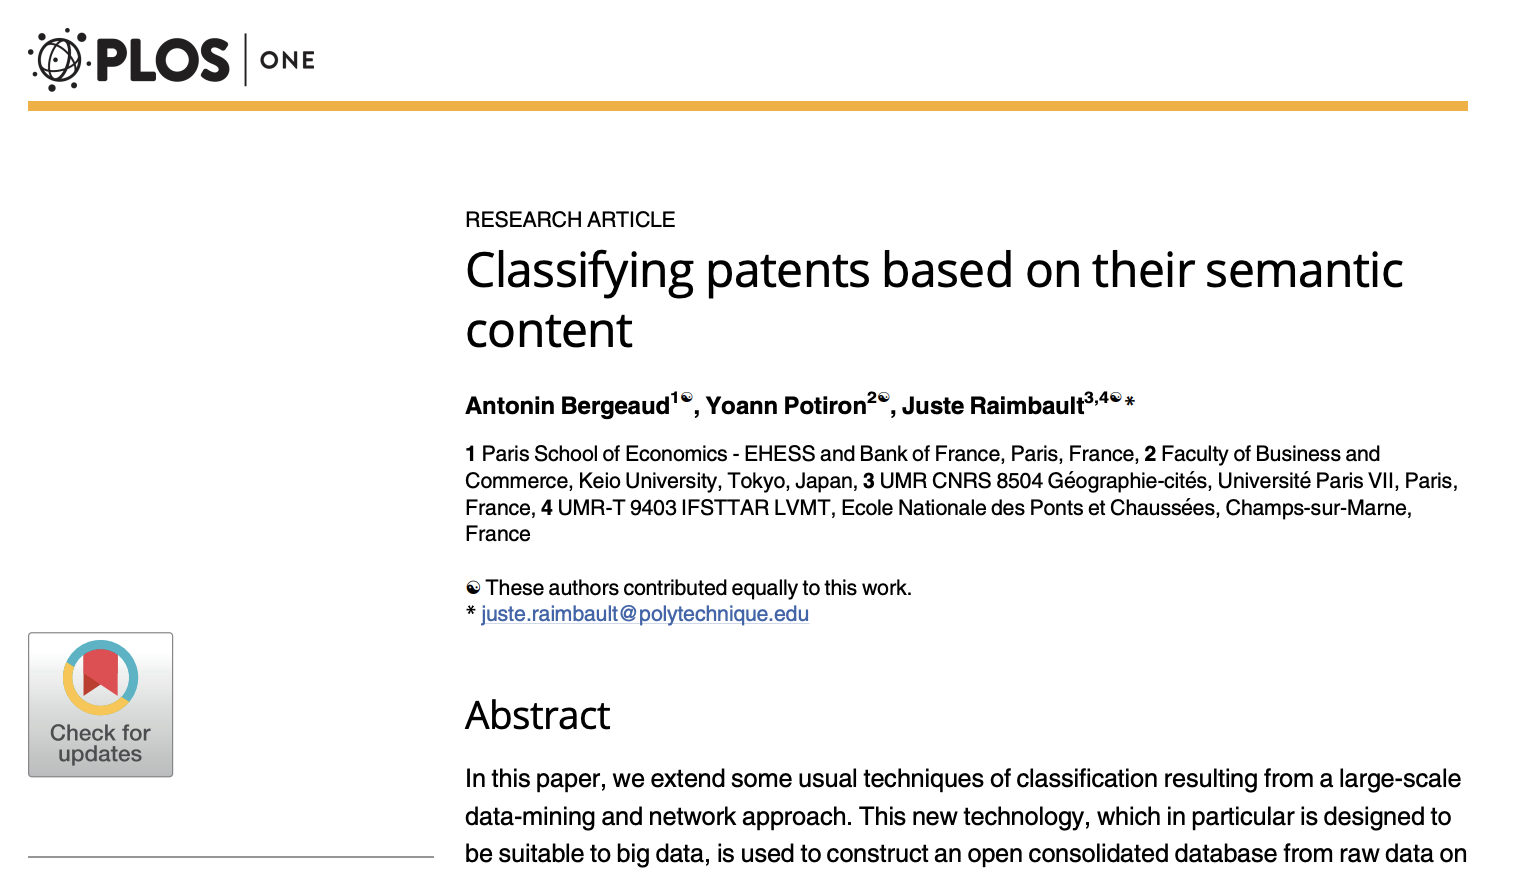
\includegraphics[width=\linewidth]{figures/patents_paper.png}

}



\sframe{Why study patents?}{
%\justify

$\rightarrow$ Although imperfect, patents are the most commonly used measure of innovation in economics

$\rightarrow$ Particular case of the ecology and evolution of knowledge; diffusion of knowledge

\bigskip

\textbf{Examples:}

\begin{itemize}
\item \cite{griliches1998patent}: patent as an economic indicator
\item \cite{Youn:2015fk} interaction between technological fields; combinatorial nature of inventions
\item \cite{2016arXiv160207928B} citation network analysis to detect emerging research fronts
\item \cite{gerken2012new} \cite{tseng2007text} semantic analysis (remains limited to specific fields and time windows)
\end{itemize} 

}


\sframe{A large scale semantic insight into US patents}{
    
   
    
    \textbf{Proposed approach}
    
    
    \textit{Complement existing patent office classifications using patent semantic content}
    
    \medskip
    
    \textbf{Why?}: more endogenous, flexible and informative (?). And comparison with \emph{technological} classification to detect outliers.
    
    \bigskip
    
    \textbf{Takeaway results}
    
    \medskip
    
    $\rightarrow$ \textit{An endogenous semantic classification is constructed for the full USPTO abstracts and titles, 1976-2012}
    
    \bigskip

    $\rightarrow$ \textit{Information carried in the semantic classification is complementary to the technological classification}
    
}



\sframe{An example of classification outcome}{
    \begin{center}
	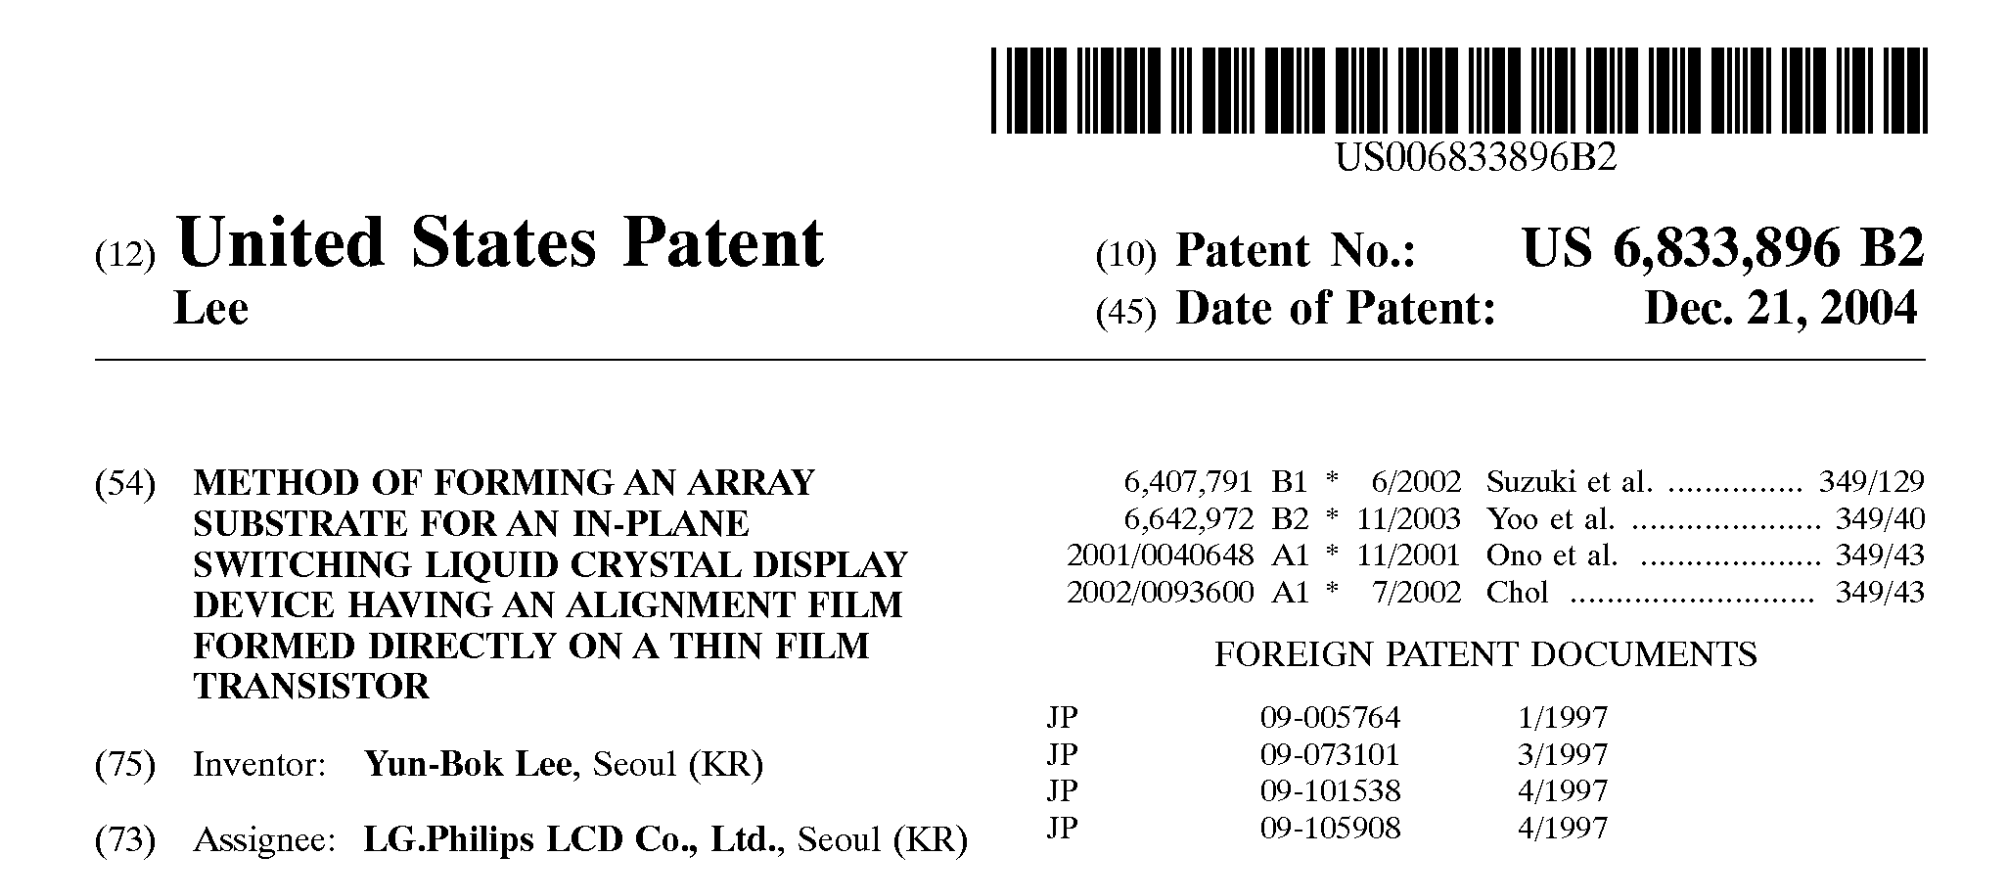
\includegraphics[width=0.8\textwidth]{figures/patents_6833896.png}
	\end{center}
	
	\medskip
	\hrule
	
\medskip
	
	\textbf{Technological classes:} 349 (Liquid Crystal Cells, Elements and Systems), 257 (electrodes)
	
	\smallskip
	
	\textbf{Prior art keywords (Google Patents):} layer, method, gate, electrode, substrate
	
	\smallskip
	
	\textbf{Most central keywords (our method):} substrat, semiconductor, insul, gate, transistor
		
}



\sframe{Descriptive statistics}{
    % summary of our database ?
    
    
    \textit{Summary statistics for the USPTO database between 1976 and 2013}
    
    \begin{itemize}
        \item 4,666,365 utility patents from 1976 to 2013
        \item 70,000 in 1976 to 278,000 in 2013
        \item 38,756,292 citation links (84\% of within-class citations)
        \item 270,877 patents with no citations 5 years next to publication
    \end{itemize}
    
    Does this mean that innovation is 4 time larger en 2013 than in 1976... \alert{Not necessary}. Although definitely more specialized.

}



% !!! no source
%\sframe{Number of inventors}{
%    \begin{figure}
%        \centering
%        \includegraphics[width=0.8\linewidth]{figures/inventors.png}
%        \caption{Evolution of number of researchers and productivity of R\&D. Source: Bloom et al. (2017)}
%    \end{figure}
%}
%
%\sframe{Inventors per patent}{
%    \begin{figure}
%        \centering
%        \includegraphics[width=0.8\linewidth]{figures/inv_per_patent.png}
%        \caption{Average number of inventors per patent. Source: USPTO.}
%    \end{figure}
%    
%    (It was 1.2 in 1900). Ideas are getting harder to find?
%    
%}

\sframe{Database construction}{
    
Construction of a Database from US Patent and Trademark Office redbook 1976-2012 (full patent description), which provide raw data but on separate files and different formats

\bigskip

\textbf{Data Collection Procedure}

\begin{itemize}
\item Automatic download of raw data file
\item Parsing depending on format : \texttt{dat} or \texttt{xml} (varying schema)
\item Uniformisation and storing in MongoDB
\end{itemize}

\bigskip

$\rightarrow$ 4,666,365 patents with text data (abstract); dated by application date (current state of knowledge, differs from the granted date which implies review processes and an exogenous intervention)


}


\sframe{Extracting relevant n-grams}{
    
    % Situate regarding other classical approaches : LDA etc
    
    \textit{Text-mining in python with \texttt{nltk}~\cite{bird2006nltk}}, method adapted from
\cite{chavalarias2013phylomemetic}. Advantage over LDA: scalability and flexibility

   

\bigskip

\begin{itemize}
\item Parsing and tokenizing / pos-tagging (word functions) / stemming  with \texttt{nltk}
\item Selection of potential \textit{n-grams} (with $1 \leq n \leq 3$) with the rule $\bigcap \{NN \cup VBG \cup JJ \}$
\item Database insertion for instantaneous use (several days $\rightarrow$ 1min)
\item Estimation of \textit{n-grams} relevance, following co-occurrences statistical distribution (\textit{termhood} score as chi-2 score)
\end{itemize}

}


\sframe{Estimation of n-gram relevance}{
    
    \begin{itemize}
        \item Termhood-based selection of a fixed number of keywords $K_W \textrm{=} 100,000$ (\textit{difficulty to select terms in general})
        \item Estimation on temporal moving windows $\left[t - T_w ; t\right]$ (fixed to $T_W \textrm{=} 4y$ after sensitivity analysis)
        \item Filtering of network edge (parameter $\theta_w$), with an additional exogenous control by technological class keyword concentration to filter nodes (parameter $\theta_c$)
        \item Low sensibility to the length of the time window for the network structure  
    \end{itemize}

}


\sframe{Technical aspects}{
	
	$\rightarrow$ Temporal complexity: $\mathcal{O}\left(N_P\right)$ for keyword extraction and co-occurrences (constant $l_{max}^2$); parallelization on a 60 cores server for a ``reasonable'' computation time. 
	
	\bigskip
	
	$\rightarrow$ Memory complexity: co-occurrence matrices in $\mathcal{O}\left(K_W^2\right)$; necessitates around 600Go RAM when parallelized. 
	
	\bigskip

	$\rightarrow$ Database management: MongoDB (nosql suited to big data).	
	
}


\sframe{Optimizing network structure}{
    
    
    
    \centering
    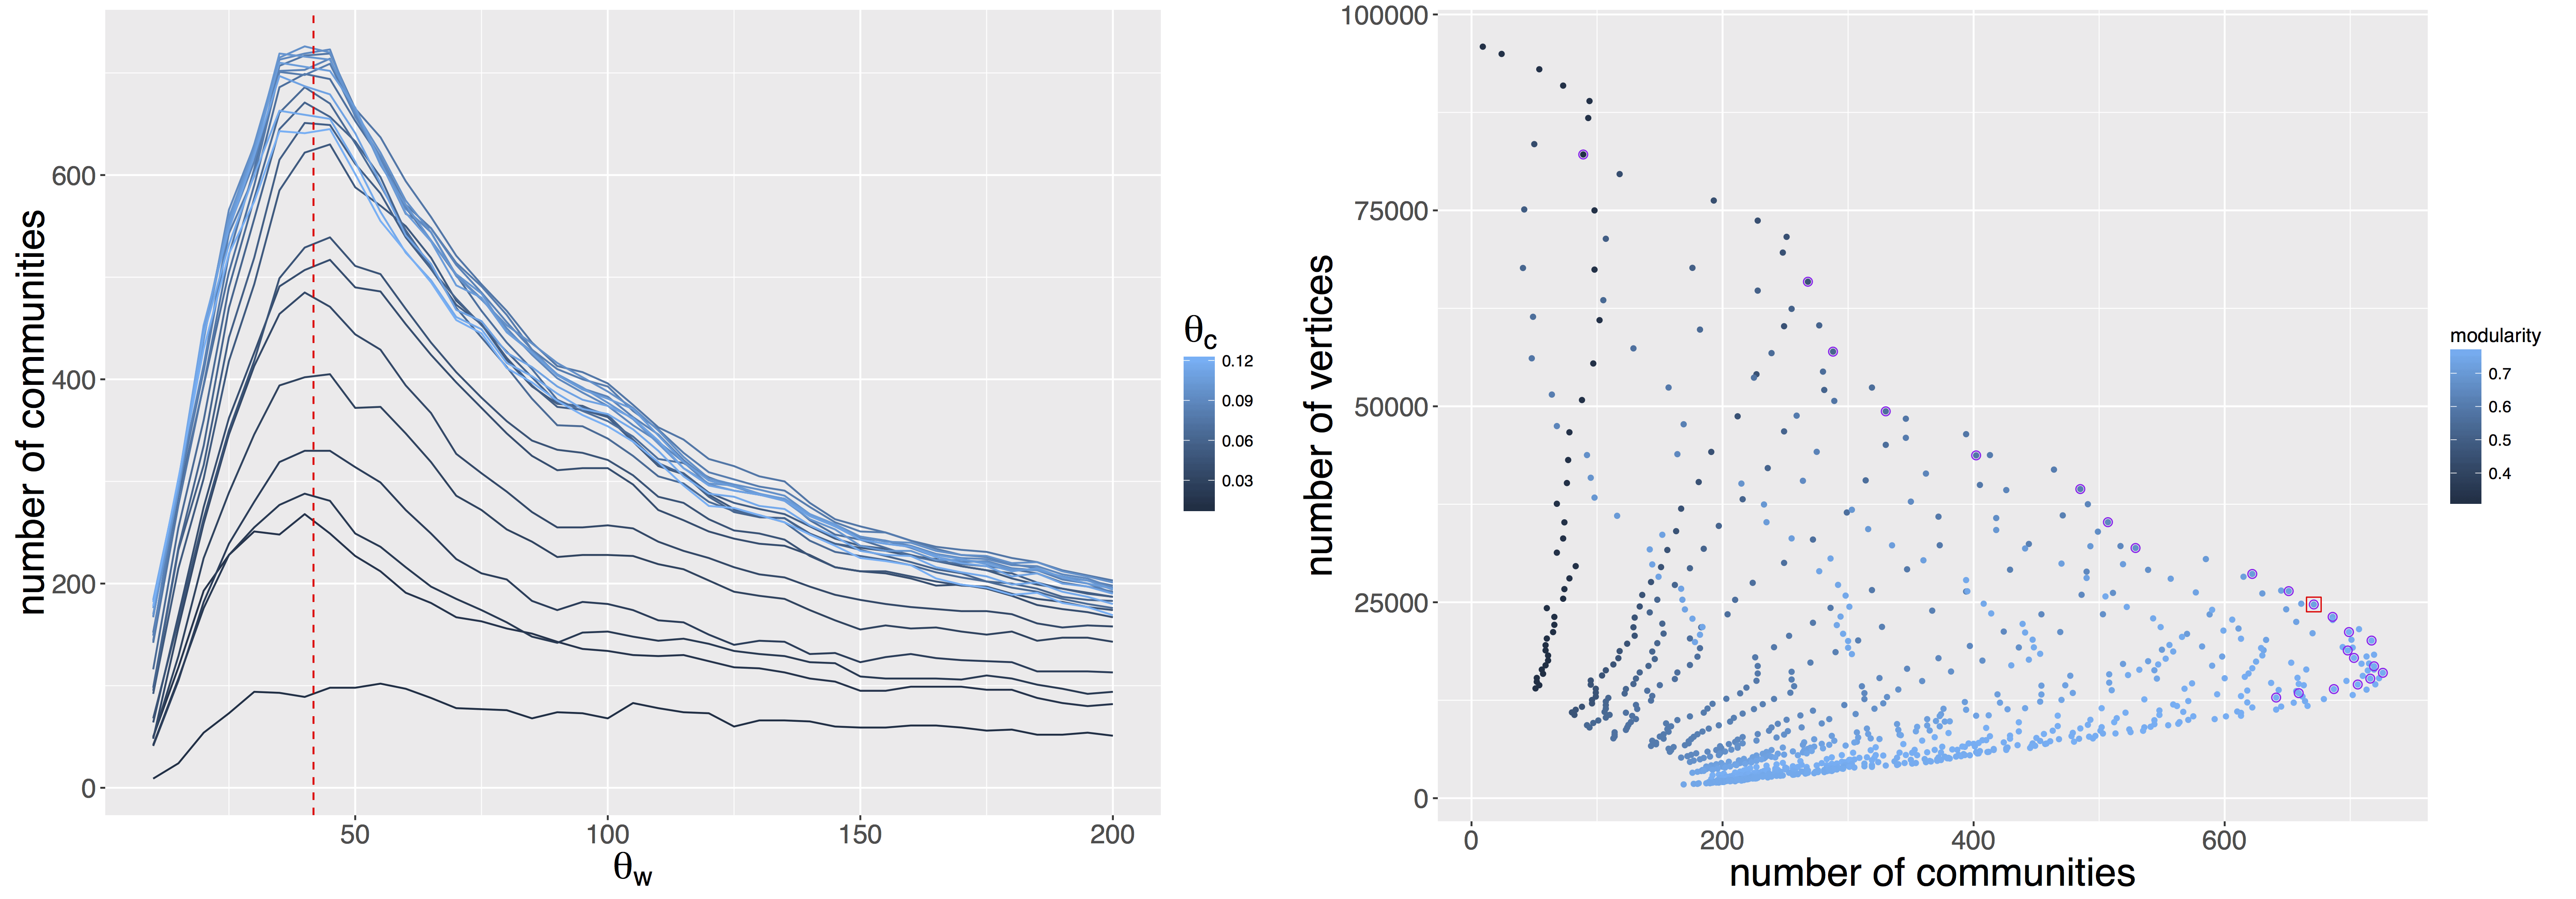
\includegraphics[width=\textwidth]{figures/patents_Fig1.png}
    
    \medskip
    
    \textit{Pareto optimization on cutoff parameters with the objectives of modularity, size and number of communities}
    
}



\sframe{Semantic network visualization (2000-2004)}{


   \centering
    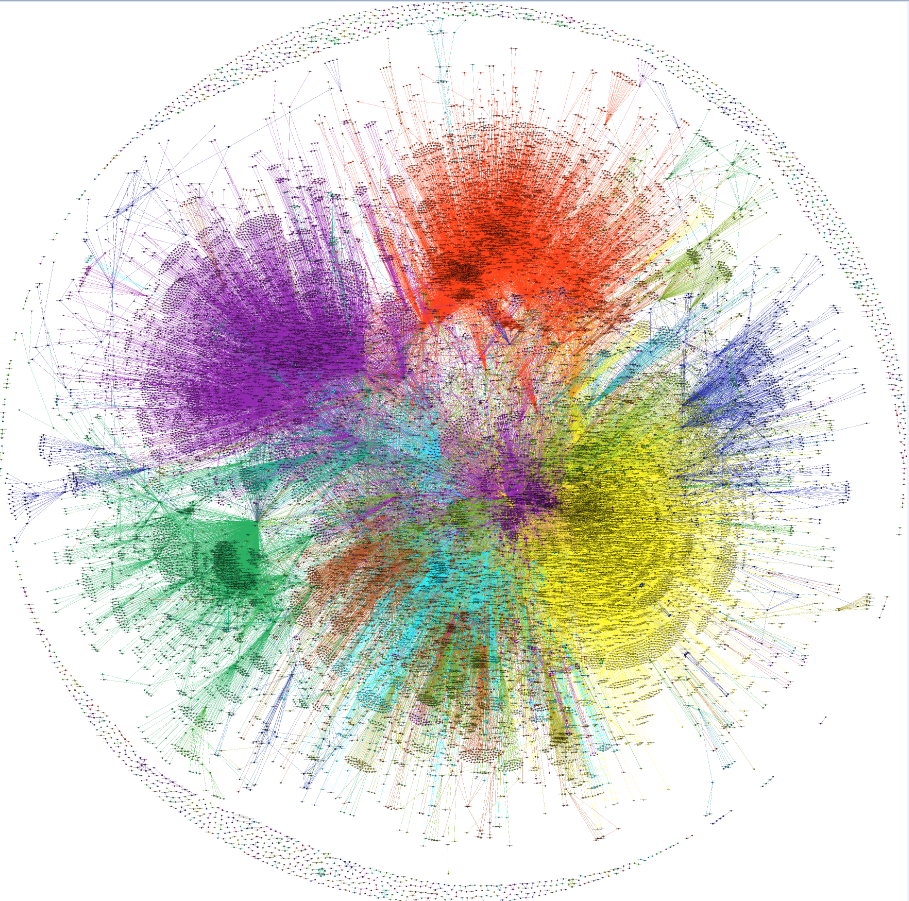
\includegraphics[height=0.85\textheight]{figures/patents_Fig2.png}
    
}
    
    
\sframe{Classes Examples (2000-2004)}{

%\justify

% discuss on naming class here

\begin{itemize}
\item Memory devices : \texttt{semiconductor memori devic; memori cell plural; memori cell transistor; layer ferroelectr}
\item Chemical analysis : \texttt{time-of-flight mass spectromet; chromatograph column; ion trap mass}
\item Particular steel : \texttt{martensit; austenit stainless steel}
\item Laser : \texttt{emit laser beam; vertic caviti surfac; vcsel}
\item Sewing : \texttt{circular knit machin; stitch; sew machin; embroideri}
\item Lithography : \texttt{lithograph mask; project beam radiat; heat-sensit; planograph print plate}
\item Tobacco : \texttt{cigarett filter; cigarett pack; tobacco; tobacco rod}
\end{itemize}

}


\sframe{Size of classes}{
   \centering
    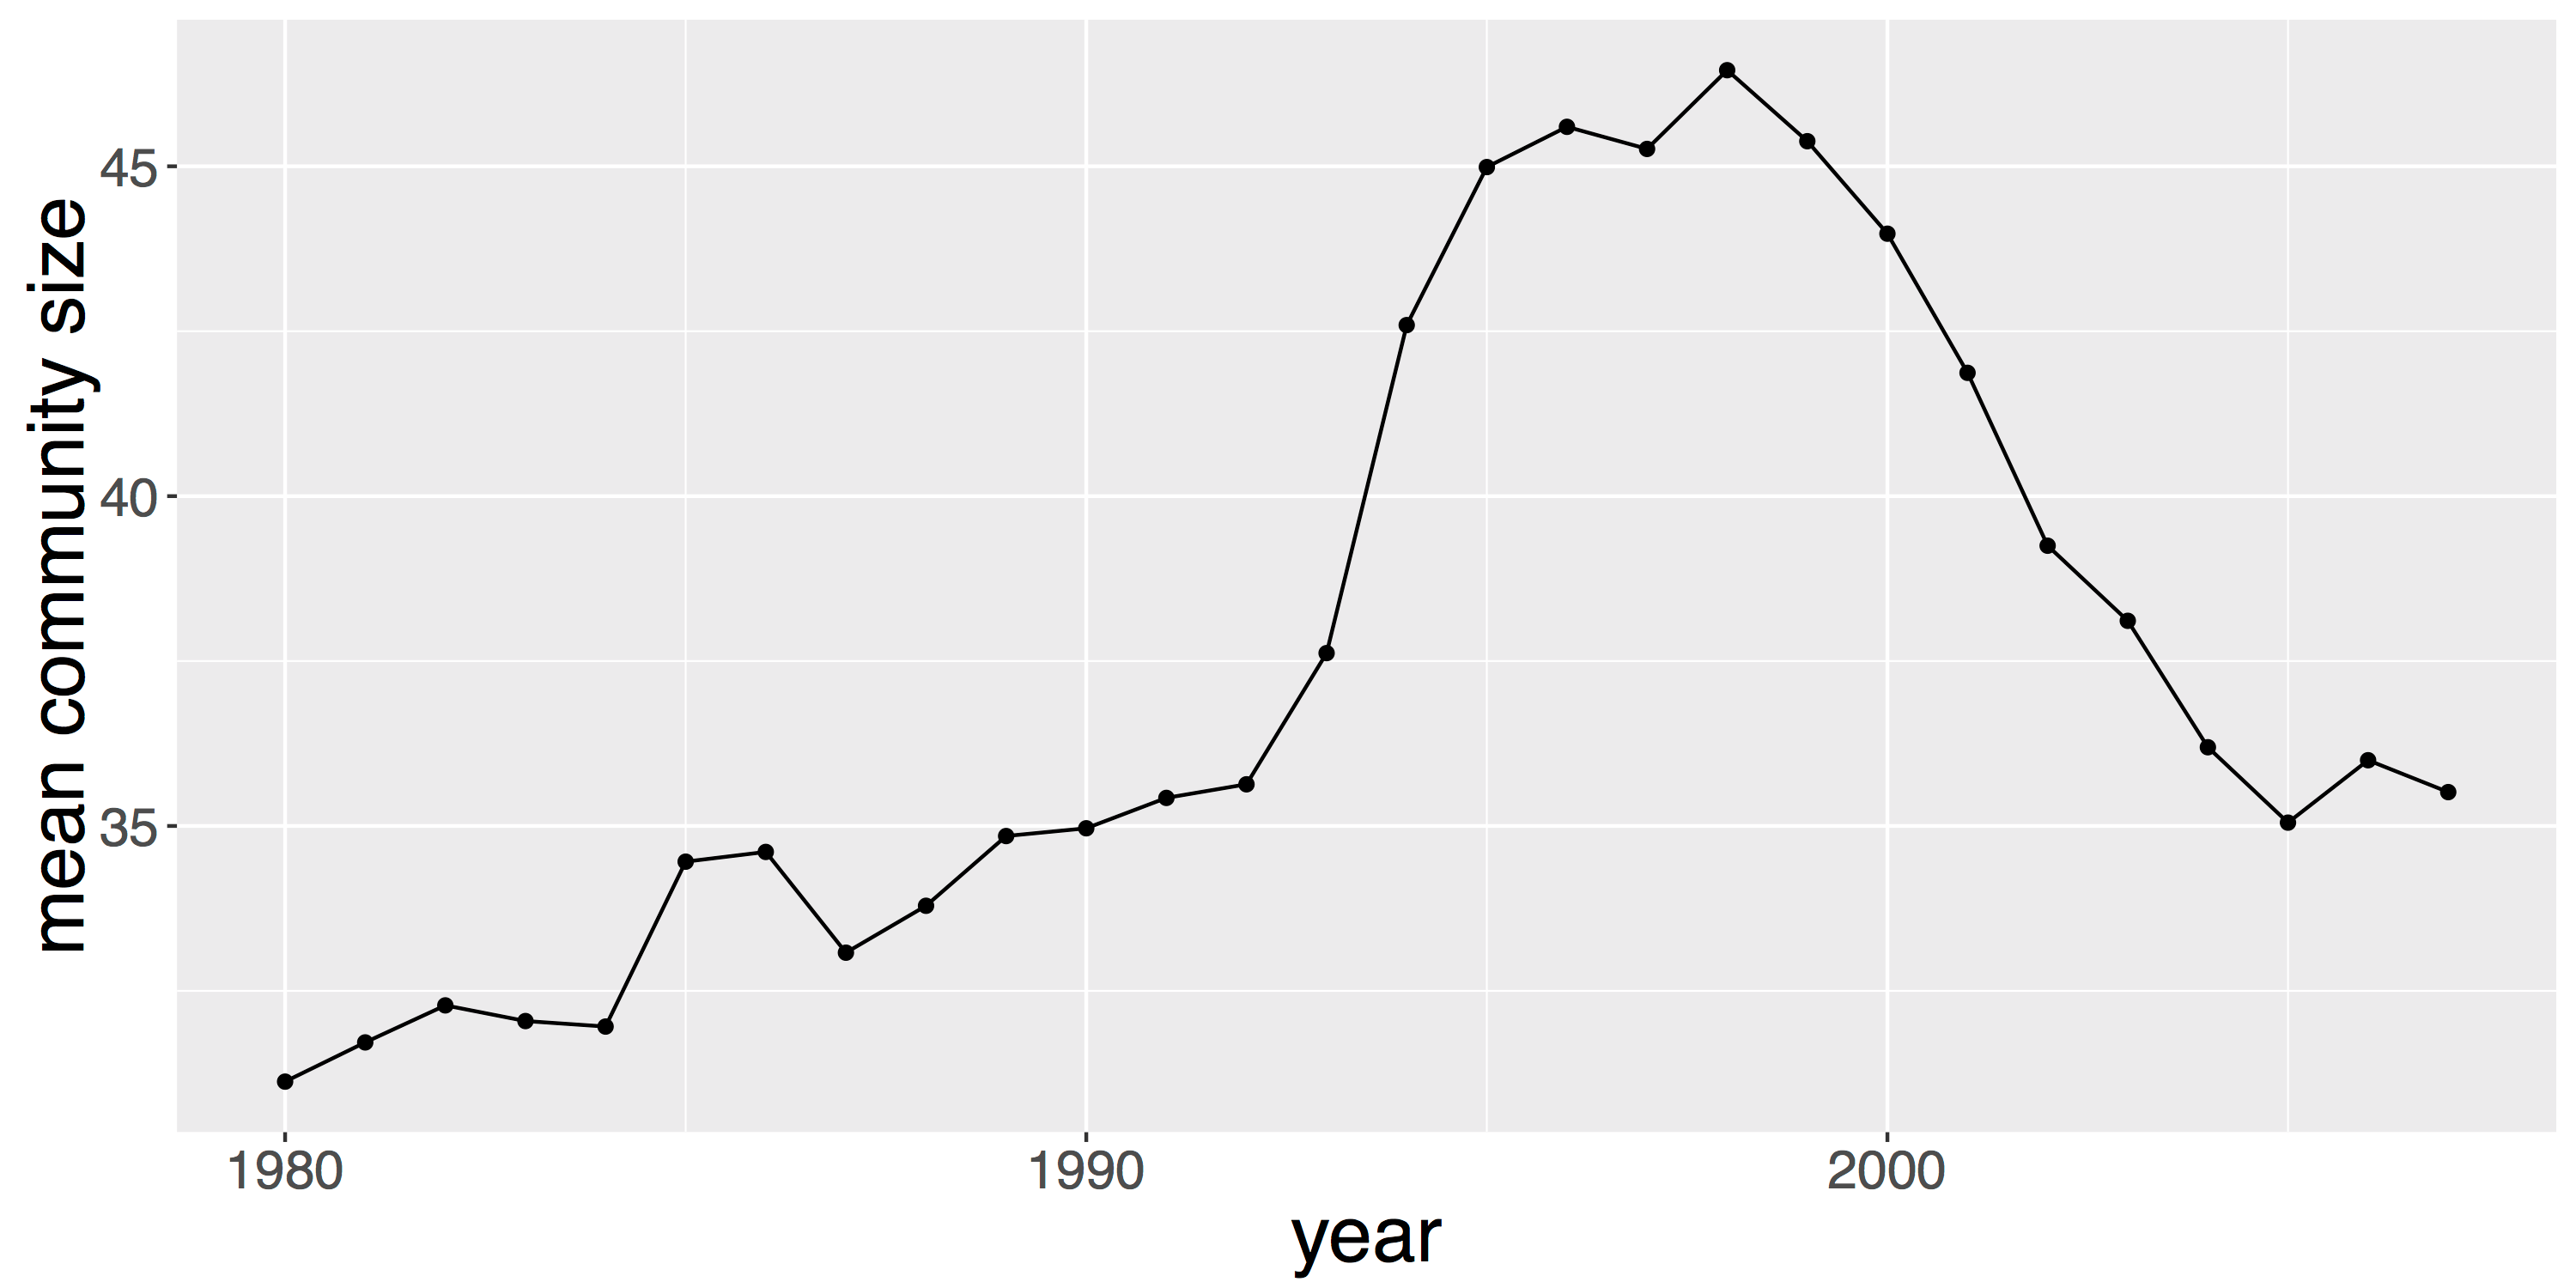
\includegraphics[width=\textwidth]{figures/patents_Fig3.png}
    
    \medskip
    
    \textit{A peak in average class size around 1998}
    
}



\sframe{Hierarchical class structure}{


   \centering
    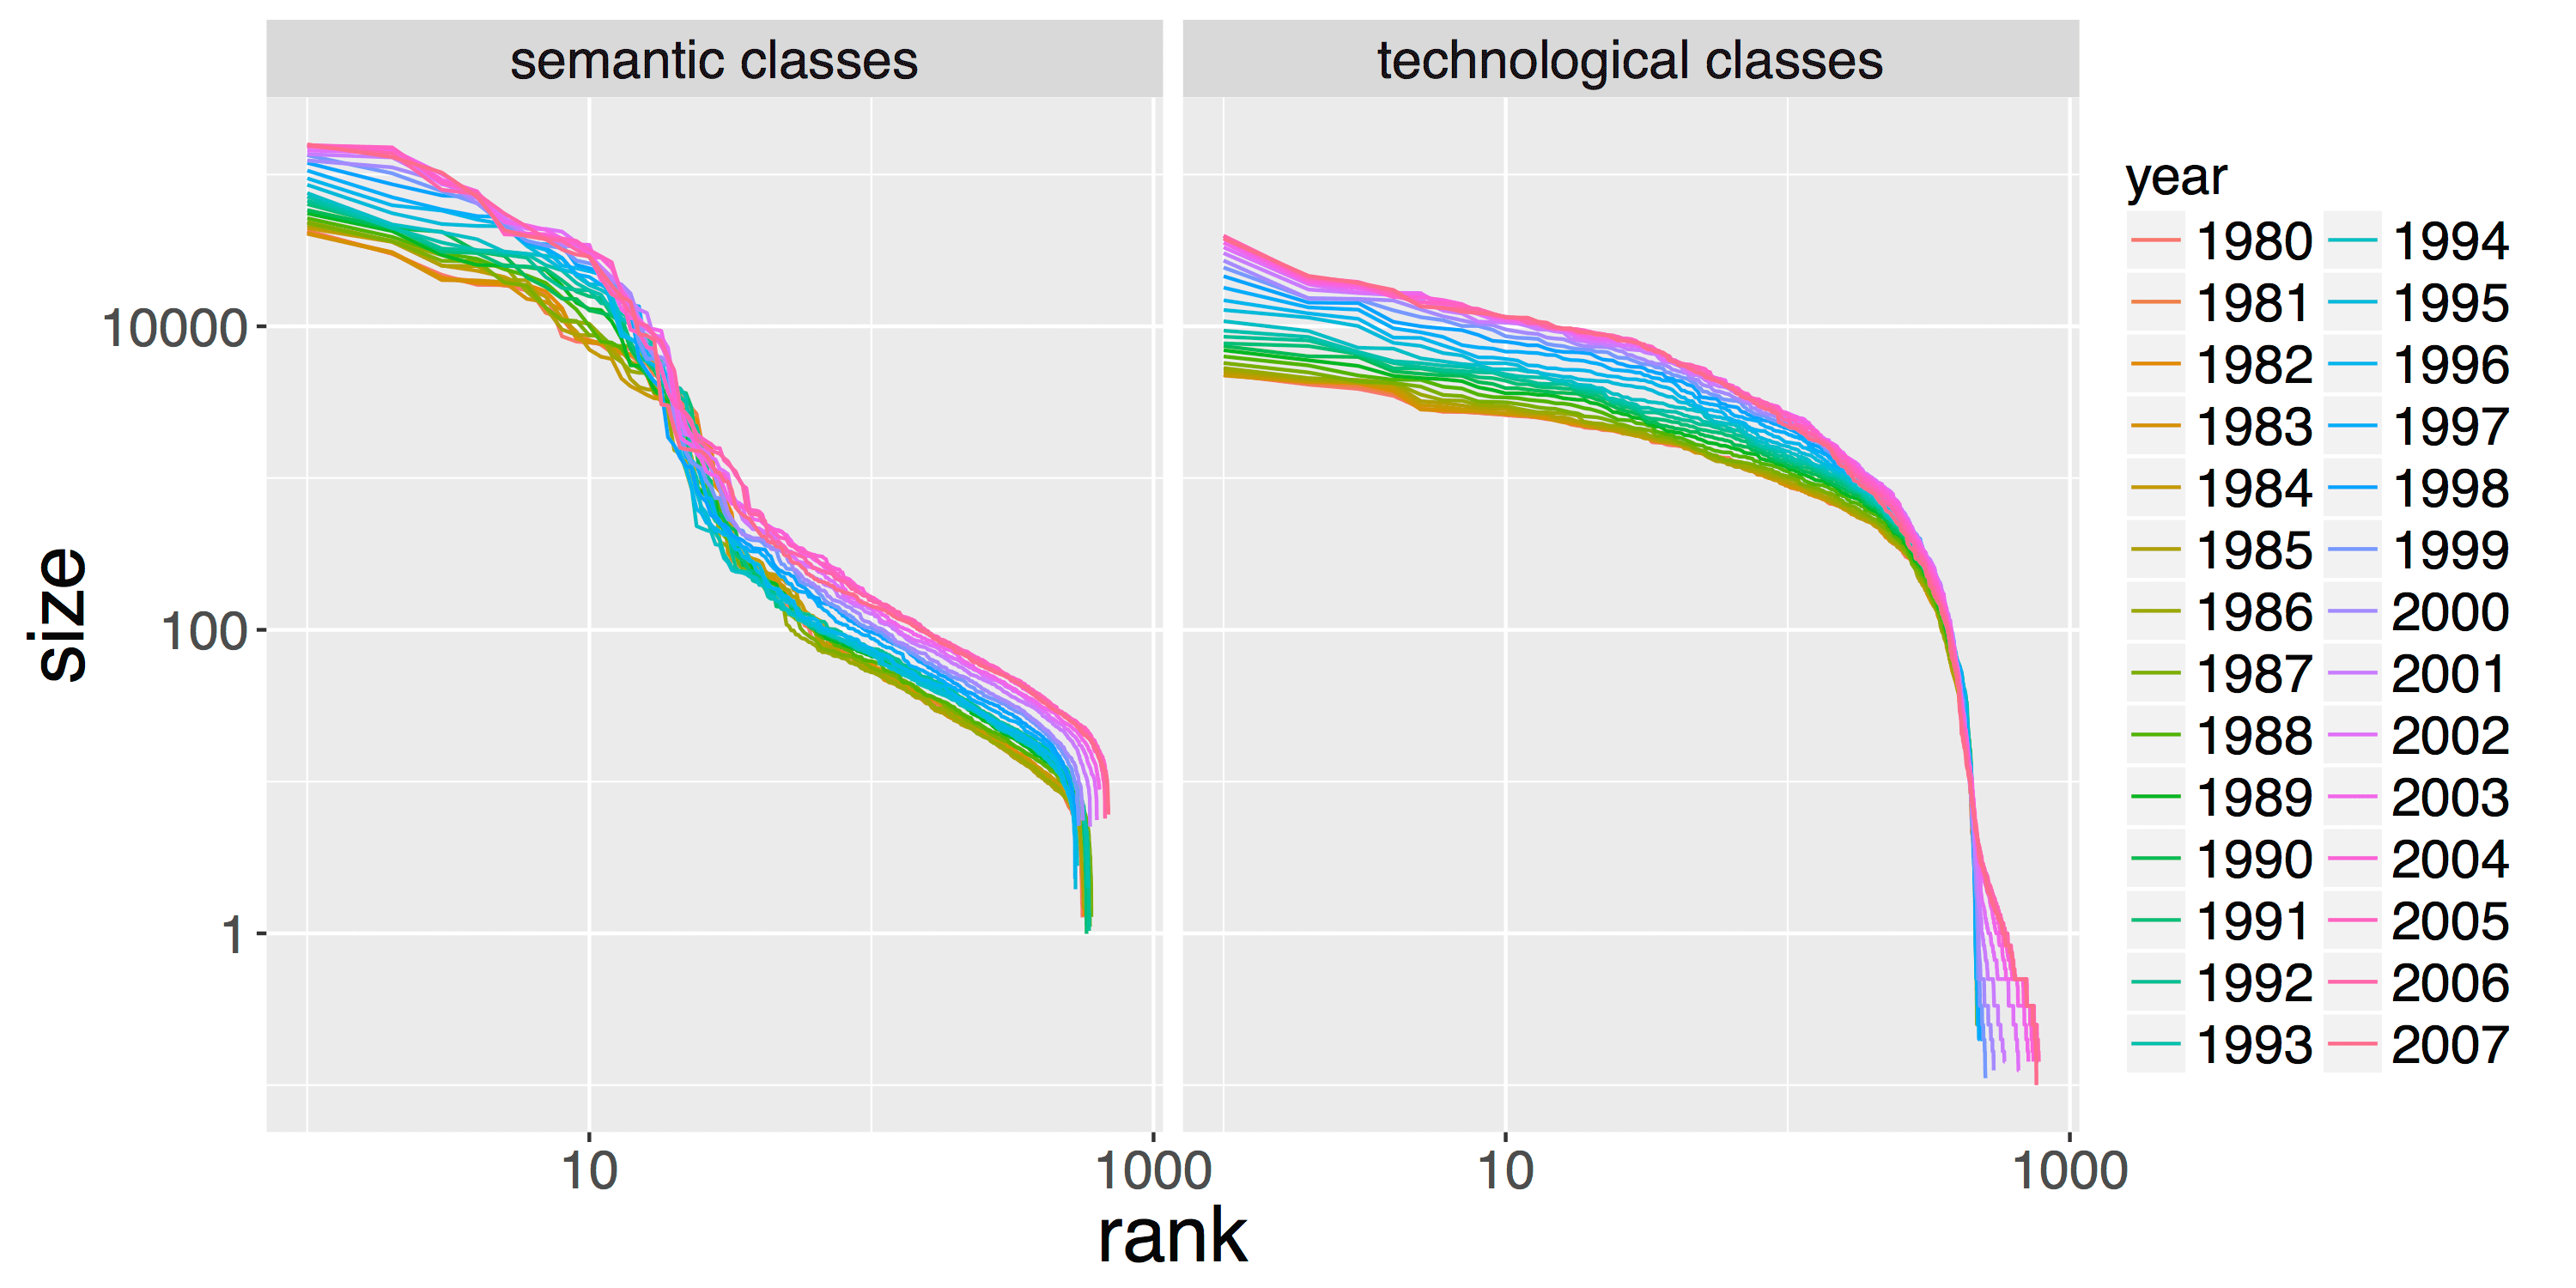
\includegraphics[width=\textwidth]{figures/patents_Fig4.png}
    
    \medskip

    \textit{Fat-tail distribution of class size for both classification, closer to a power-law for semantic classes}
 
 
}




\sframe{Patent measures}{
    
    \textit{Diversity}
    \[
D_i^{(z)} \textrm{=} 1 - \sum_{j =1}^{N^{(z)}} {p_{ij}^2}, \text{ with } z \in \{tec, sem\}
	\]
    
    \medskip

	\textit{Originality and Generality}

	\[
O_i^{(z)} \textrm{=} \displaystyle 1 - \sum_{j \textrm{=}1}^{N^{(z)}}{\left(\frac{\displaystyle \sum_{i' \in I_i}{p_{i'j}}}{\displaystyle \sum_{k =1}^{N^{(z)}}{\displaystyle \sum_{i' \in I_i}{p_{i'k}}}}\right)^2}
\text{ and } G_i^{(z)} \textrm{=} \displaystyle 1 - \sum_{j \textrm{=}1}^{N^{(z)}}{\left(\frac{\displaystyle \sum_{i' \in \tilde{I}_i}{p_{i'j}}}{\displaystyle \sum_{k =1}^{N^{(z)}}{\displaystyle \sum_{i' \in \tilde{I}_i}{p_{i'k}}}}\right)^2}
\]
    
    
}

\sframe{Evolution of patent diversities}{


   \centering
    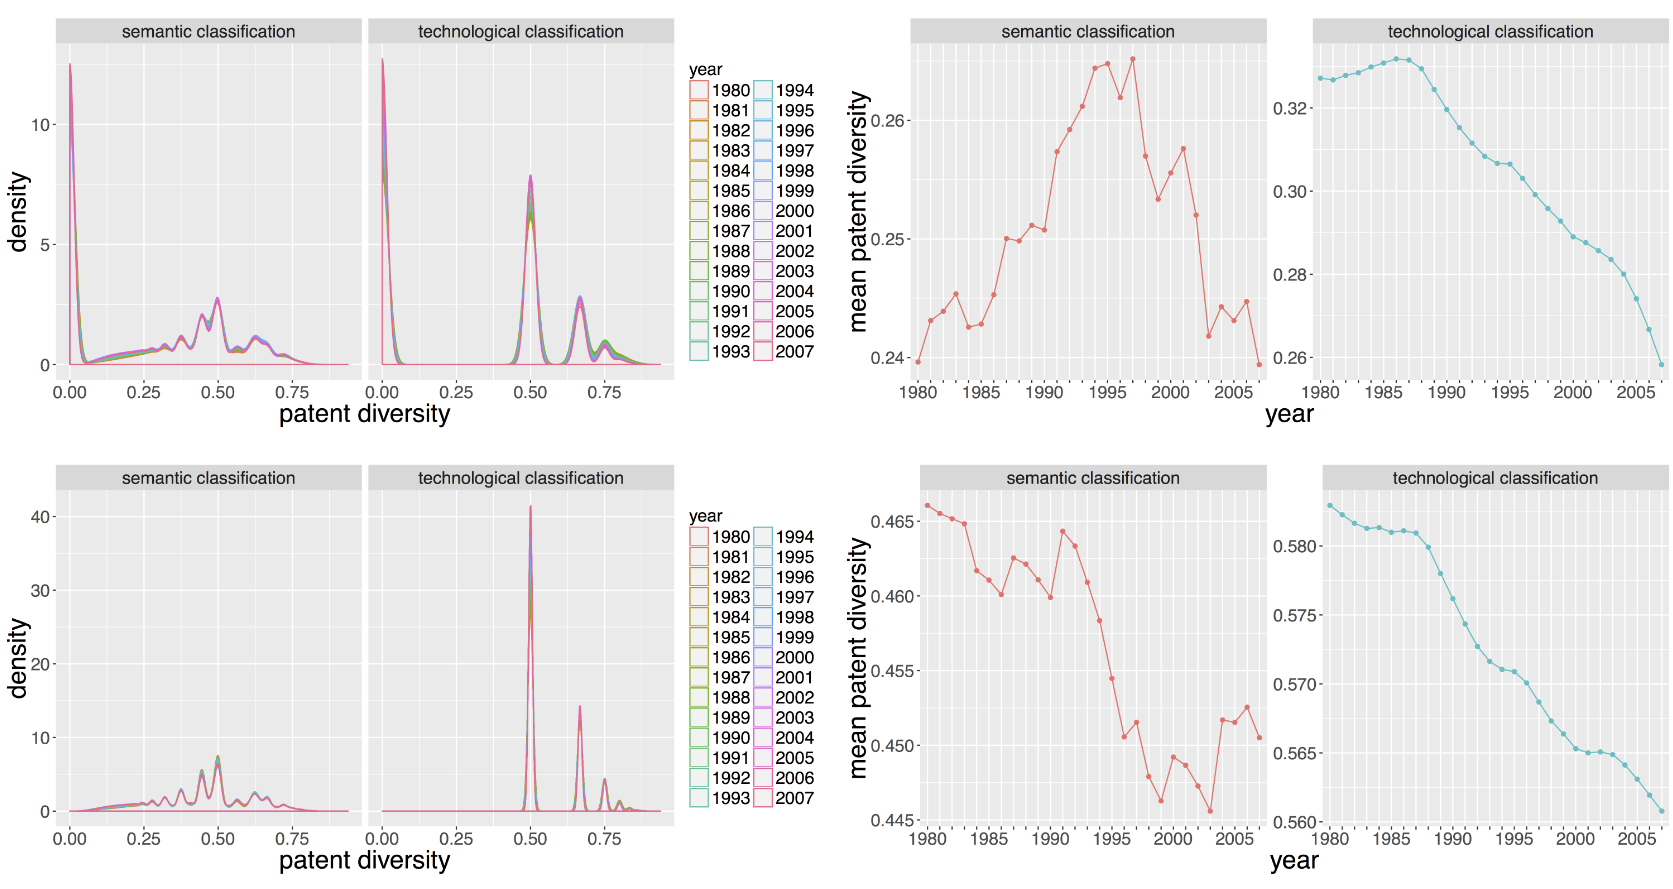
\includegraphics[width=\textwidth]{figures/patents_Fig5.png}
    
    \medskip

    \textit{General increase in average invention specialization seen both for semantic and technological; semantic regime shift in 1996} 
  
}


\sframe{Originality and generality measures}{
    \centering
    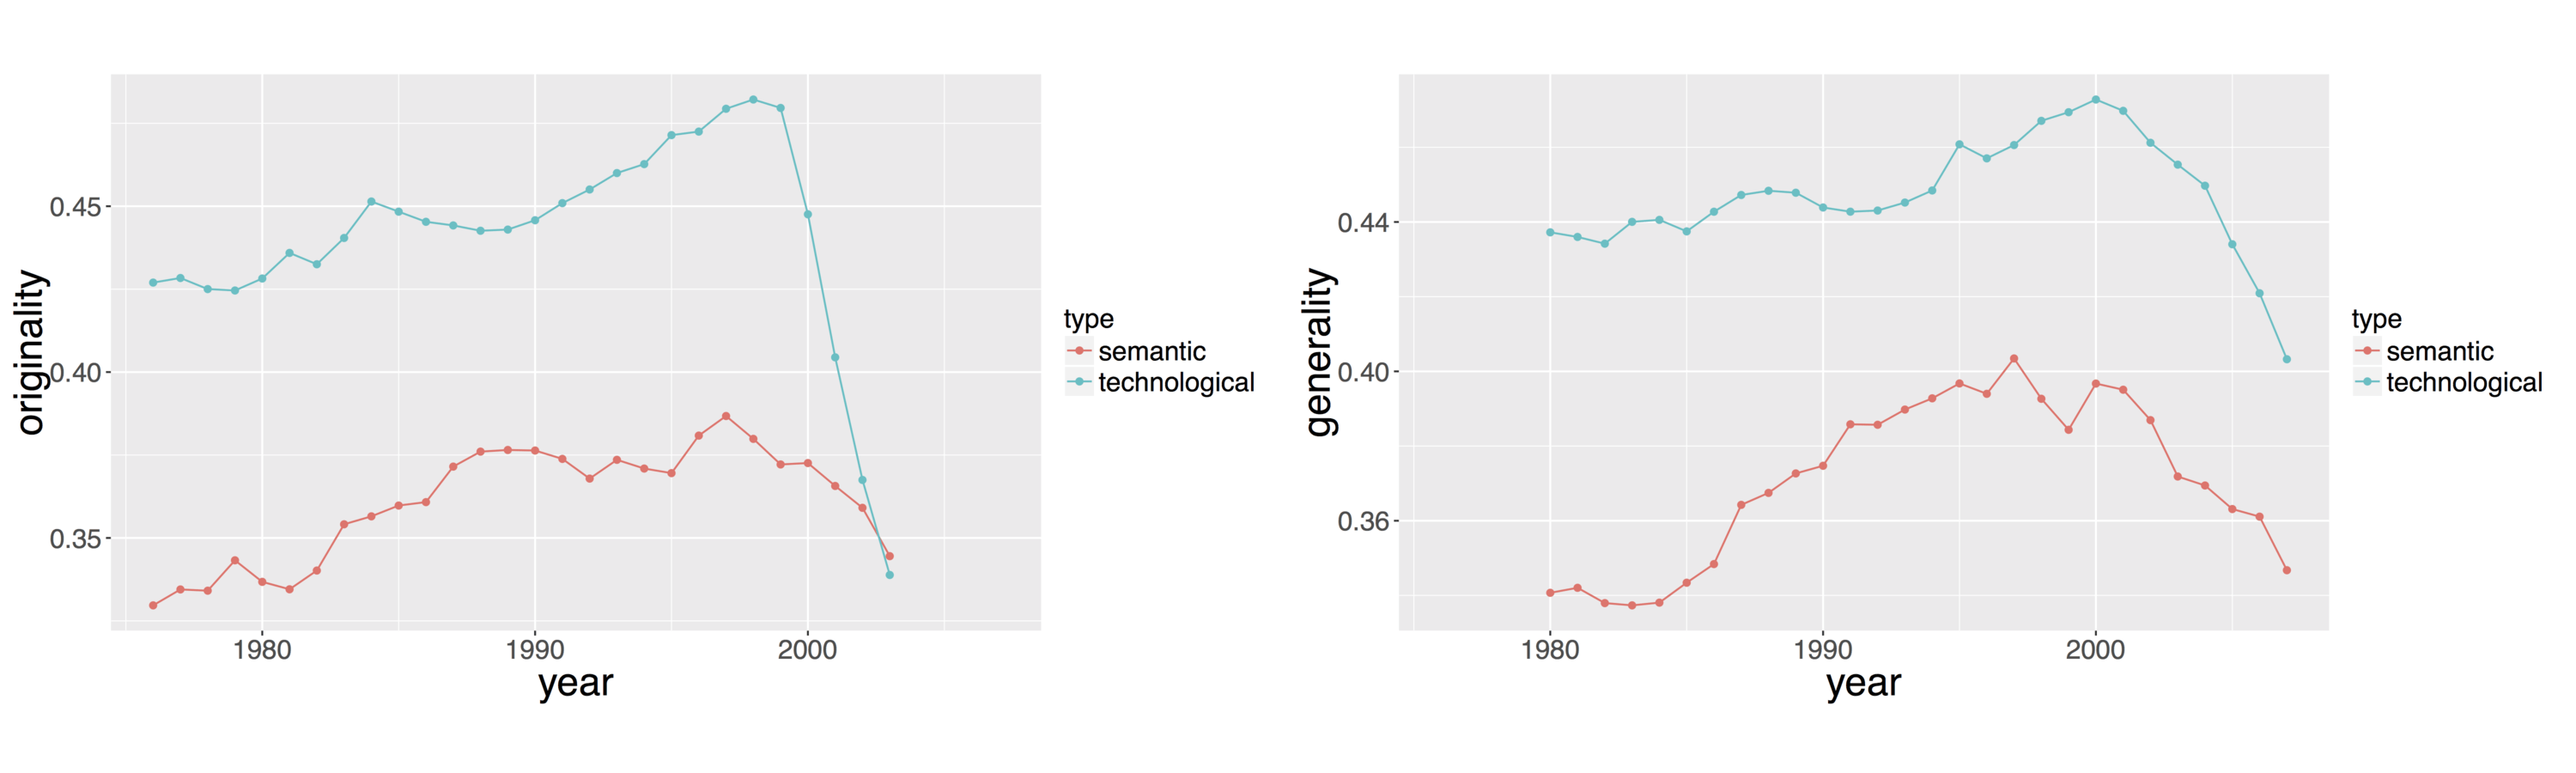
\includegraphics[width=\textwidth]{figures/patents_Fig6.png}
    
    \medskip
    
    \textit{Systematically lower originality and generality (citation-based measures) for the semantic classification (consistent with the higher modularity shown thereafter).}
    

}


\sframe{Interaction between classes: intra-classification overlaps}{
   \centering
    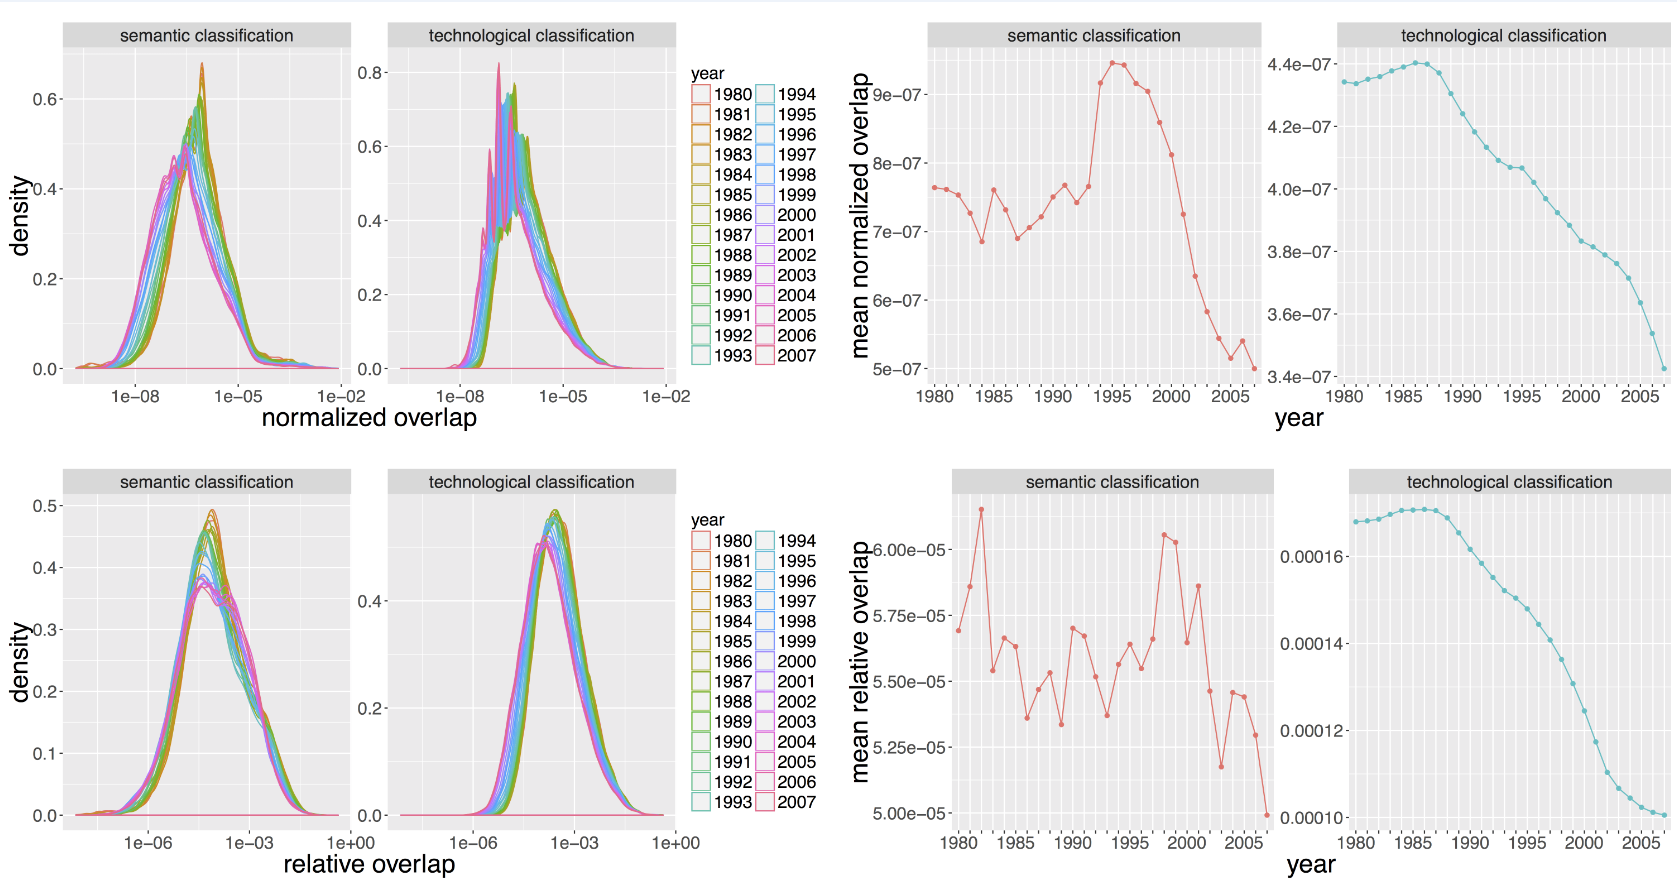
\includegraphics[width=\textwidth]{figures/patents_Fig7.png}
    
    \medskip

    % techno : increasing specializatino trend
    % semantic : consistent with 1996 breakpoint in the structure of technologies - rq : how to control specifically that it is not an artifact of the method / or biased by sizes ?
    
    \textit{Increased technological specialization; qualitative regime shift confirmed in 1996 for the semantic classification}
   
   
}

\sframe{Inter-classification overlaps}{
  
   \begin{center}
    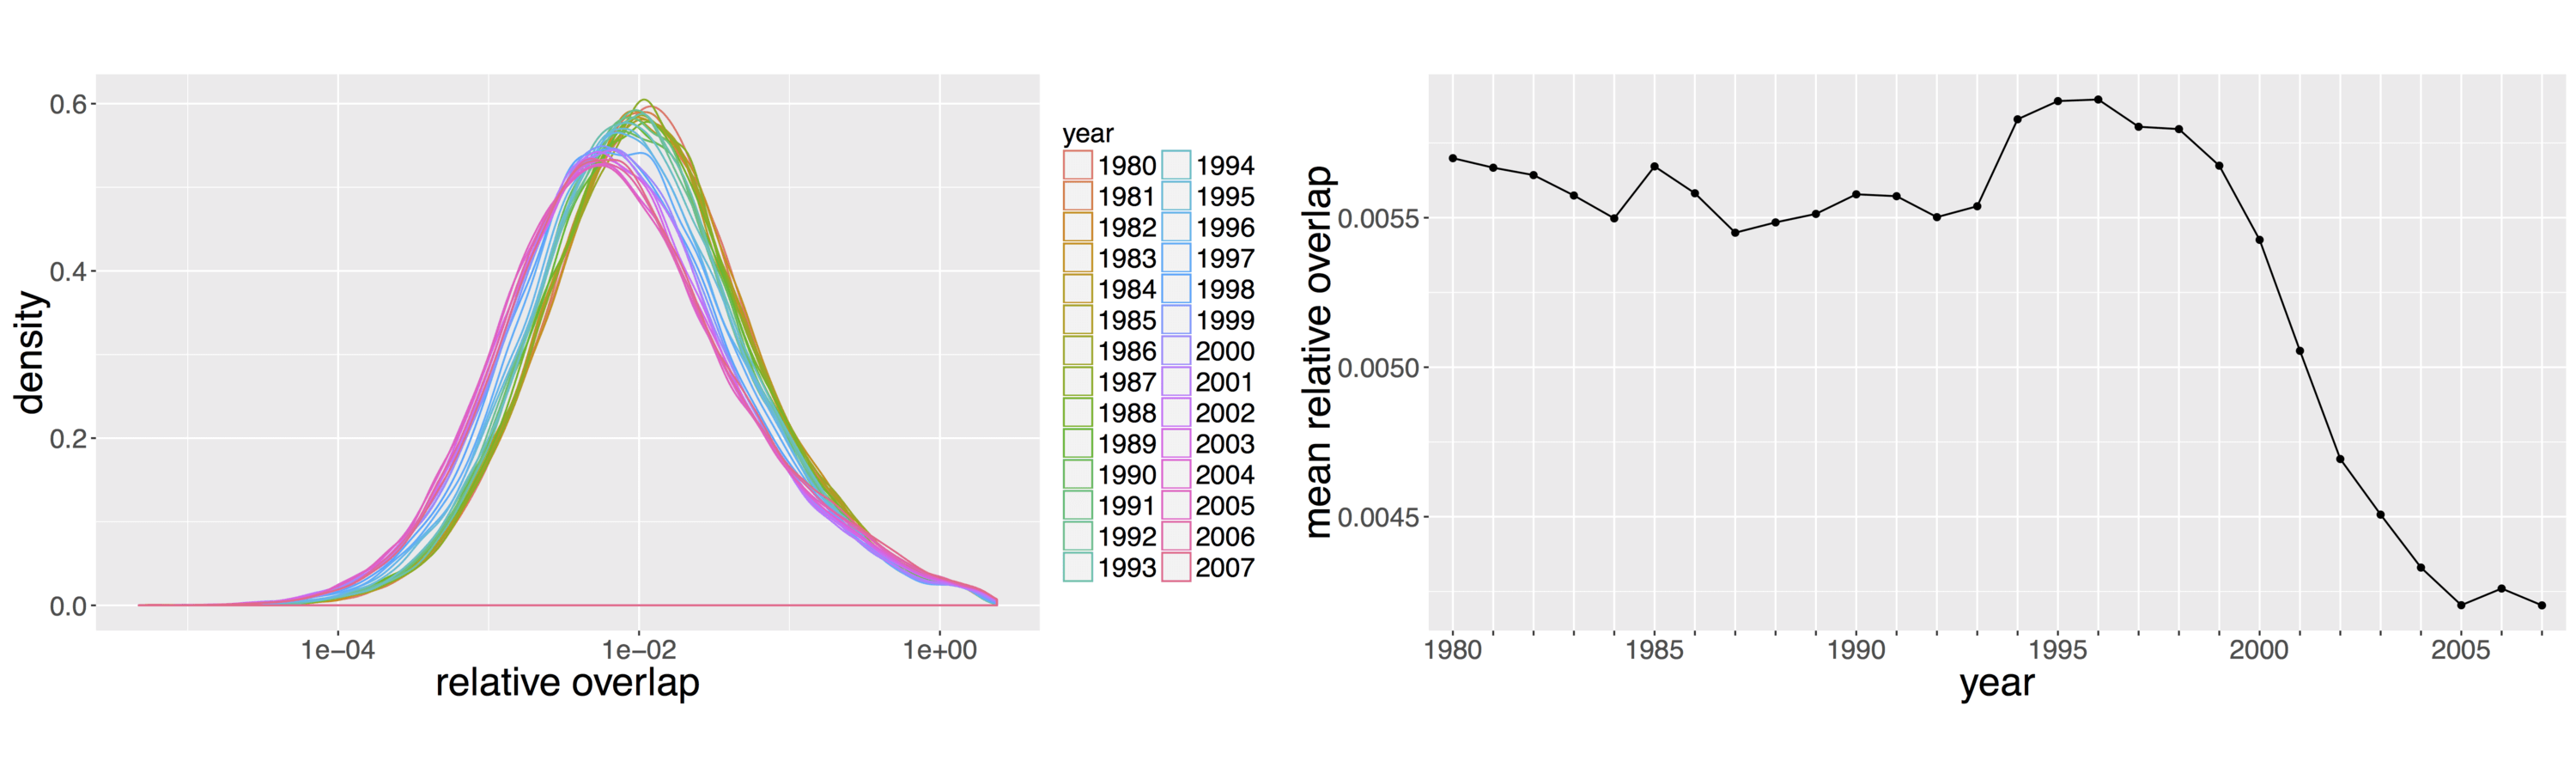
\includegraphics[width=\textwidth]{figures/patents_Fig8.png}
  	\end{center}
    
    \medskip

    \textit{Constant then decreasing average overlap between technological and semantic classes; confirms the change in nature of inventions around 1996.} 
    
    \smallskip
    
    $\rightarrow$ an impact of new information technologies (regarding knowledge production: from expert and contextualized to automatized search in references e.g.) ? Linked to structural changes in economy (increase in firm concentration since 90s) ?
    
    
}



\sframe{Definition of modularities}{


    Directed simple modularity \cite{nicosia2009extending}
    \[
Q_d^{(z)} \textrm{=} \displaystyle \frac{1}{N_P}\sum_{1\leq i,j\leq N_P}\left[A_{ij} - \frac{k_{i}^{in}k_{j}^{out}}{N_P}\right]\delta\left(c_i,c_j\right),
\]


\bigskip

Multi-class modularity:

\[
\displaystyle Q_{ov}^{(z)} \textrm{=} \frac{1}{N_P} \sum_{c \textrm{=} 1}^{N^{(z)}} \sum_{1\leq i,j \leq N_P}\left[F\left(p_{ic},p_{jc}\right)A_{ij} - \frac{\beta_{i,c}^{out}k_i^{out}\beta_{j,c}^{in}k_j^{in}}{N_P}\right],
\]
where
\[
 \beta_{i,c}^{out}\textrm{=}  \frac{1}{N_P} \displaystyle \sum_j F\left(p_{ic},p_{jc}\right) \text{ and } \beta_{j,c}^{in} \textrm{=} \frac{1}{N_P} \displaystyle \sum_i F\left(p_{ic},p_{jc}\right).
\]

}



\sframe{Modularity of classifications}{

   \begin{center}
    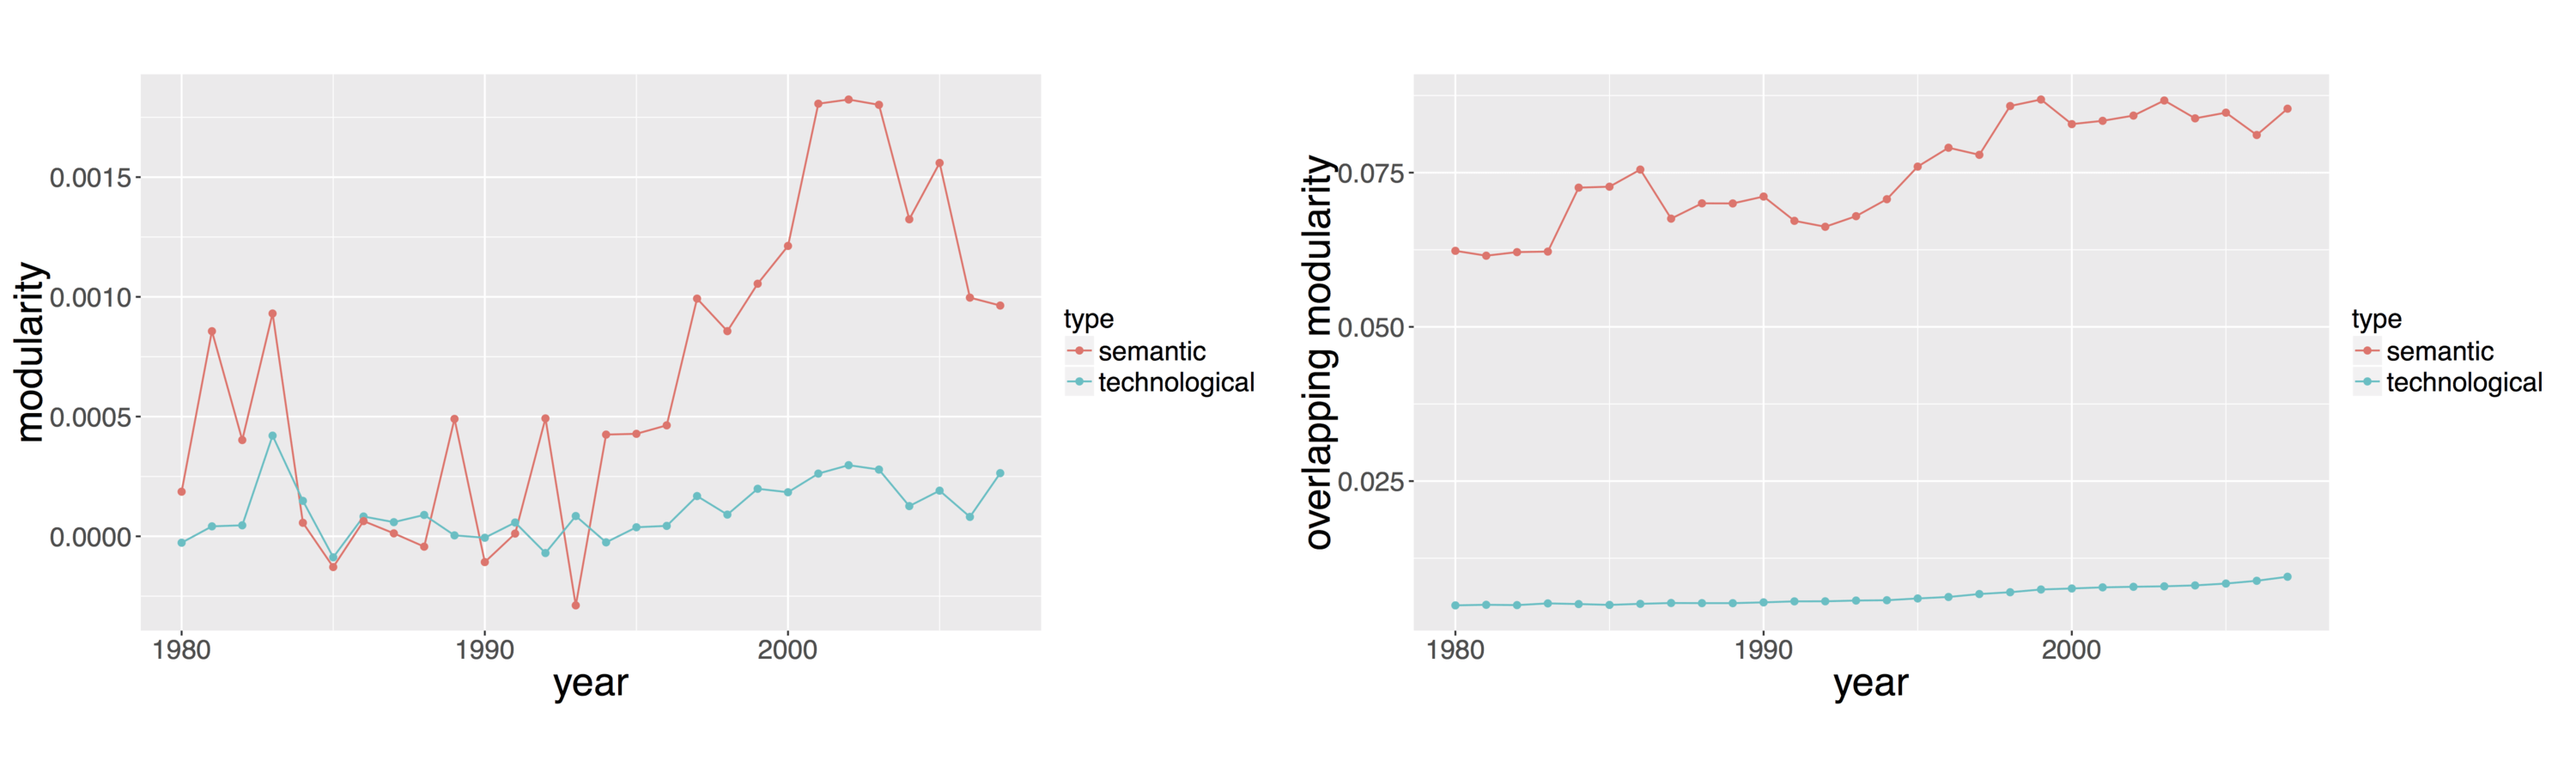
\includegraphics[width=\textwidth]{figures/patents_Fig9.png}
    \end{center}
    
    \medskip
    
    \textit{Semantic classification is more significant regarding the structure of the citation network, both for single-class and multi-class modularities (confirmed statistically using a simple Stochastic Block Model).}
    
}

\sframe{Stochastic Block Modeling to evaluate consistency of classifications}{
\begin{itemize}
    \item   We complete the analysis by developing a statistical model aiming at quantifying performance of both technological and semantic classification systems
    \item Intuitively, we look at within class citations proportion (for both technological and semantic approaches)
    \item Question: is the semantic classification better at predicting future within class citations? \\
    $\longrightarrow$ short answer is \alert{yes}.
\end{itemize} 

}


\sframe{Possible developments}{

\textbf{Extensions}
    \begin{itemize}
        \item Look at the correlation between patent quality indicators and centrality indices.
        \item Use patent-firm matching to study a \emph{firm-level} semantic network.
        \item Extending the analysis to other patent offices (EPO/JPO).
    \end{itemize}
    
    \medskip
    
\textbf{Economic}
    \begin{itemize}
        \item Linking semantic measures to values of firms
        \item Can semantic proximity helps understand M\&A?
        \item Firms trajectories in relation to their life-cycle
    \end{itemize}

\medskip

\textbf{Technology}
\begin{itemize}
    \item Measure of complementarity between technology?
    \item Possible application to detection of emerging research fronts
    \item An interactive exploration of semantic content?
\end{itemize}


}



\section{Exploration of an interdisciplinary scientific landscape}


% This same method was adapted to scientific papers by (Raimbault, 2019) and used to study patterns of interdisciplinarity of papers published in the Cybergeo geography journal. These works confirm the complementarity of both citation and semantic approaches.


% Cybergeo papper SCIM
% Patterns of interdisciplinarity in science can be quantified through complementary dimen- sions. This paper studies as a case study the scientific environment of a generalist journal in Geography, Cybergeo, in order to introduce a novel methodology combining citation network analysis and semantic analysis. We collect a large corpus of around 200,000 arti- cles with their abstracts and the corresponding citation network that provides a first citation classification. Relevant keywords are extracted for each article through text-mining, allow- ing us to construct a semantic classification. We study the qualitative patterns of relations between endogenous disciplines within each classification, and finally show the comple- mentarity of classifications and of their associated interdisciplinarity measures. The tools we develop accordingly are open and reusable for similar large scale studies of scientific environments. Our contribution therefore provides, besides the methodology, a new way to construct open databases and study journals for which data are difficult to obtain.
% Citation network · Semantic network · Interdisciplinarity · Geography


\sframe{Similar method applied to a scientific corpus}{


\textit{Study around the interdisciplinary geography journal Cybergeo}

\bigskip
\bigskip

\centering

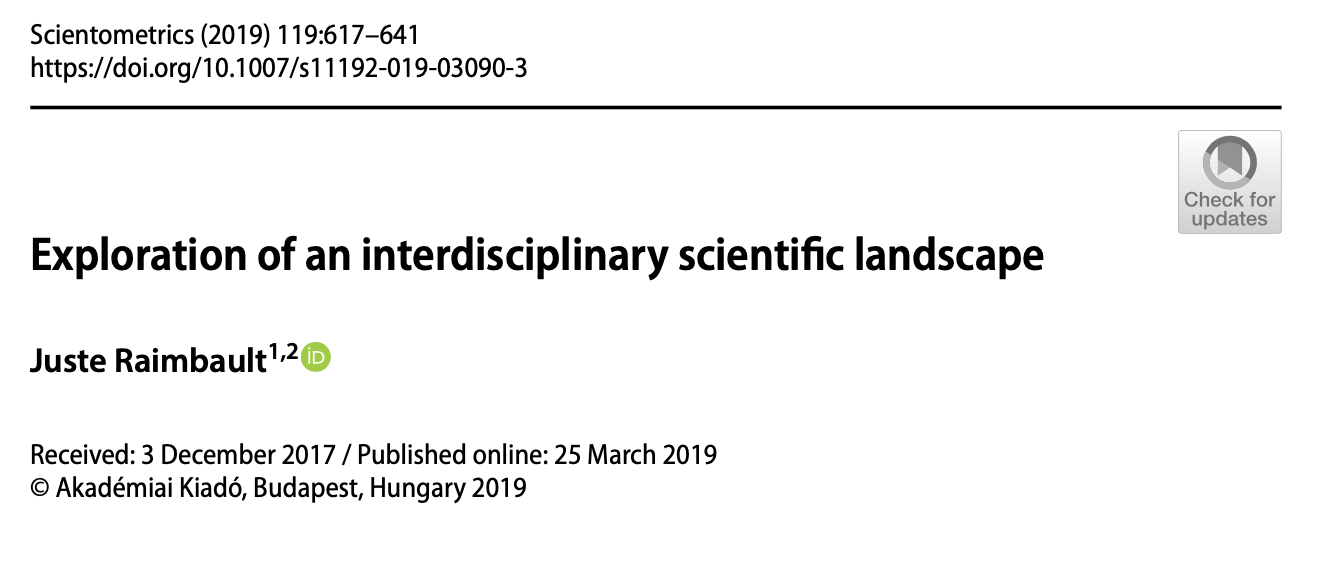
\includegraphics[width=0.9\textwidth]{figures/scim_paper.png}

}





\sframe{Interdisciplinarity}{



\justify

\textit{Importance of interdisciplinary approaches for knowledge itself but also to solve complex issues such as global change and sustainability}

\bigskip

$\rightarrow$ different types of integration between disciplines in theory 

\cite{chavalarias2009french} and in practice \cite{dupuy2015sciences}

\bigskip
\bigskip

\centering


\includegraphics[width=0.49\textwidth]{figures/scim_erc.png}\hspace{0.5cm}

\includegraphics[width=0.45\textwidth]{figures/scim_miti.png}


}

\sframe{Scientometrics}{


Quantitative Studies of Science beyond bibliometrics \cite{cronin2014beyond}:

\medskip

\begin{itemize}
	\item Maps of science \cite{borner2012design}\cite{leydesdorff2009global}
	\item Modeling science dynamics \cite{borner2011modeling}
	\item Modeling social processes in science \cite{edmonds2011simulating}
	\item Citation \cite{shibata2008detecting}, co-authorship, semantic networks \cite{gaumont2017methods}
	\item Quantitative epistemology \cite{chavalarias2013phylomemetic}
\end{itemize}


}


\sframe{Defining and measuring interdisciplinarity}{

% Definitions of interdisciplinarity itself and indicators to measure it have already been tackled by a large body of literature. Huutoniemi et al. (2010) recall the difference between multidisciplinary (an aggregate of works from different disciplines) and inter- disciplinary (implying a certain level of integration) approaches. They construct a qual- itative framework to classify types of interdisciplinarity, and for example distinguish empirical, theoretical and methodological interdisciplinarities.Wagner et al. (2011) find that knowledge integration is crucial for interdisciplinarity, and that it can occur at different levels, from the single scientist to the research team or the field. Hall et al. (2008) confirm the role of the social aspect in potential interdiscipli- nary collaborations, by proposing to include the readiness to collaborate in the evalua- tion of corresponding research units. The multidimensionnal aspect of interdisciplinar- ity is confirmed even within a specific field such as literature (Austin et al. 1996). Beside these different conceptual approaches to interdisciplinarity, there exist several methodological means to measure it, of which we now give an overview. A first way to quantify interdisciplinarity of a set of publications is to look at the proportion of disciplines outside a main discipline in which they are published, as Rinia et al. (2002) do for the evaluation of projects in physics, complementary with judgement of experts. Porter et al. (2007) designate this measure as specialization, and compare it with a measure of integration, also called the Rao-Stirling index, which is given by the spread of citations done by a paper within the different Subject Categories (classification of the Web of Knowledge). Larivière and Gingras (2010) use it on a Web of Science corpus to show the existence of an optimal intermediate level of interdisciplinarity for the cita- tion impact within a five year window. A similar work is done in Larivière and Gingras (2014), focusing on the evolution of measures on a long time range. The influence of missing data on this index is studied by Moreno et al. (2016), providing an extended framework taking into account uncertainty. Other indices based on citation practices have been introduced, such as by Rod- ríguez (2017) which proposes an entropy-based index to classify the behavior of journal regarding knowledge import or export. Zhang et al. (2016) recall mathematical proper- ties that need to be verified by diversity indices (such as symmetry or scale-invariance), and proposes that Hill-type indices are more relevant than entropy. Mugabushaka et al. (2016) show that most of existing indices are a particular cases of Leinster-Cobbold diversity indices, which correspond to a third generation of indices to measure diversity in ecology. Leydesdorff and Rafols (2011) compare different indi- ces at the level of journals, and show that they appear to capture different dimensions of this phenomenon in a complementary way. The use of bottom-up network measures has also been proposed to quantify inter- disciplinary research: Porter and Rafols (2009) combine the integration index with a mapping technique which consists in visualisation of synthetic networks constructed by co-citations between disciplines. Leydesdorff (2007) shows that the betweenness centrality is a relevant indicator of interdisciplinarity, when considering appropriate citation neighborhood. A multilayer network approach was proposed in Omodei et al. (2017), using bipartite networks of papers and scholars, in order to produce measures of interdisciplinarity using generalized centrality measures. Rafols and Meyer (2009) combine diversity indices with measures of network coherence, which capture the inte- gration of knowledge.
% Semantic analysis and interdisciplinarity
%A particular entry to the quantification of interdisciplinarity is semantic analysis of docu- ments. Nichols (2014) uses Latent Dirichlet Allocation topic modeling to characterize interdisciplinarity of awards in particular sciences. Palchykov et al. (2016) do the same for papers in physics based on concept extraction from full texts, and show that the endog- enous classes differ from the top-down subjects classification. Semantic networks are oth- erwise well studied in social sciences, such as for example Gurciullo et al. (2015) which analyze semantic networks of political debates. Bouveyron et al. (2018) introduce a block model for network clustering which includes textual information of nodes. Boyack et al. (2011) benchmark several text-based clustering methods. Semantic analysis can be coupled with other dimensions, and in particular citation net- work analysis. Brás et al. (2017) study oncology by coupling the semantic aspects with institutional aspects. Zhang et al. (2010) describe cross-journals citation clusters in terms of their semantic content, but do not produce an endogenous semantic classification. Gerow et al. (2018) find that the citation influence and the discursive influence of scholars are complementary dimensions of academic success, by using topic modeling for the semantic classification of their work.


\begin{itemize}
	\item Difference between multi- and interdisciplinary, and empirical, theoretical or methodological interdisciplinarity \cite{huutoniemi2010analyzing}
	\item Specialization indices (Rao-Stirling) \cite{lariviere2010relationship}
	\item Diversity indices (Leinster-Cobbold) \cite{mugabushaka2016bibliometric}
	\item Network-based indices \cite{leydesdorff2007betweenness} \cite{rafols2009diversity}
	\item Semantic aspects of interdisciplinarity \cite{nichols2014topic} \cite{bouveyron2016stochastic}	
\end{itemize}




}


\sframe{Proposed approach}{


\textit{Difficulty to quantify interdisciplinarity (i) through multiple complementary dimensions; (ii) when data is not straightforward to gather.}

\bigskip

For a case study journal in Geography (Cybergeo, European Journal of Geography \url{https://journals.openedition.org/cybergeo/})

\medskip

$\rightarrow$ construct a database from heterogenous sources

\medskip

$\rightarrow$ quantify interdisciplinarity with citation and semantic networks


}


\sframe{Data collection}{


Data collected from heterogenous sources: journal production database, google scholar for citation links, Mendeley for abstracts.

\medskip

Refactored open source java library for data collection: \url{https://github.com/JusteRaimbault/BiblioData}

\bigskip

\centering

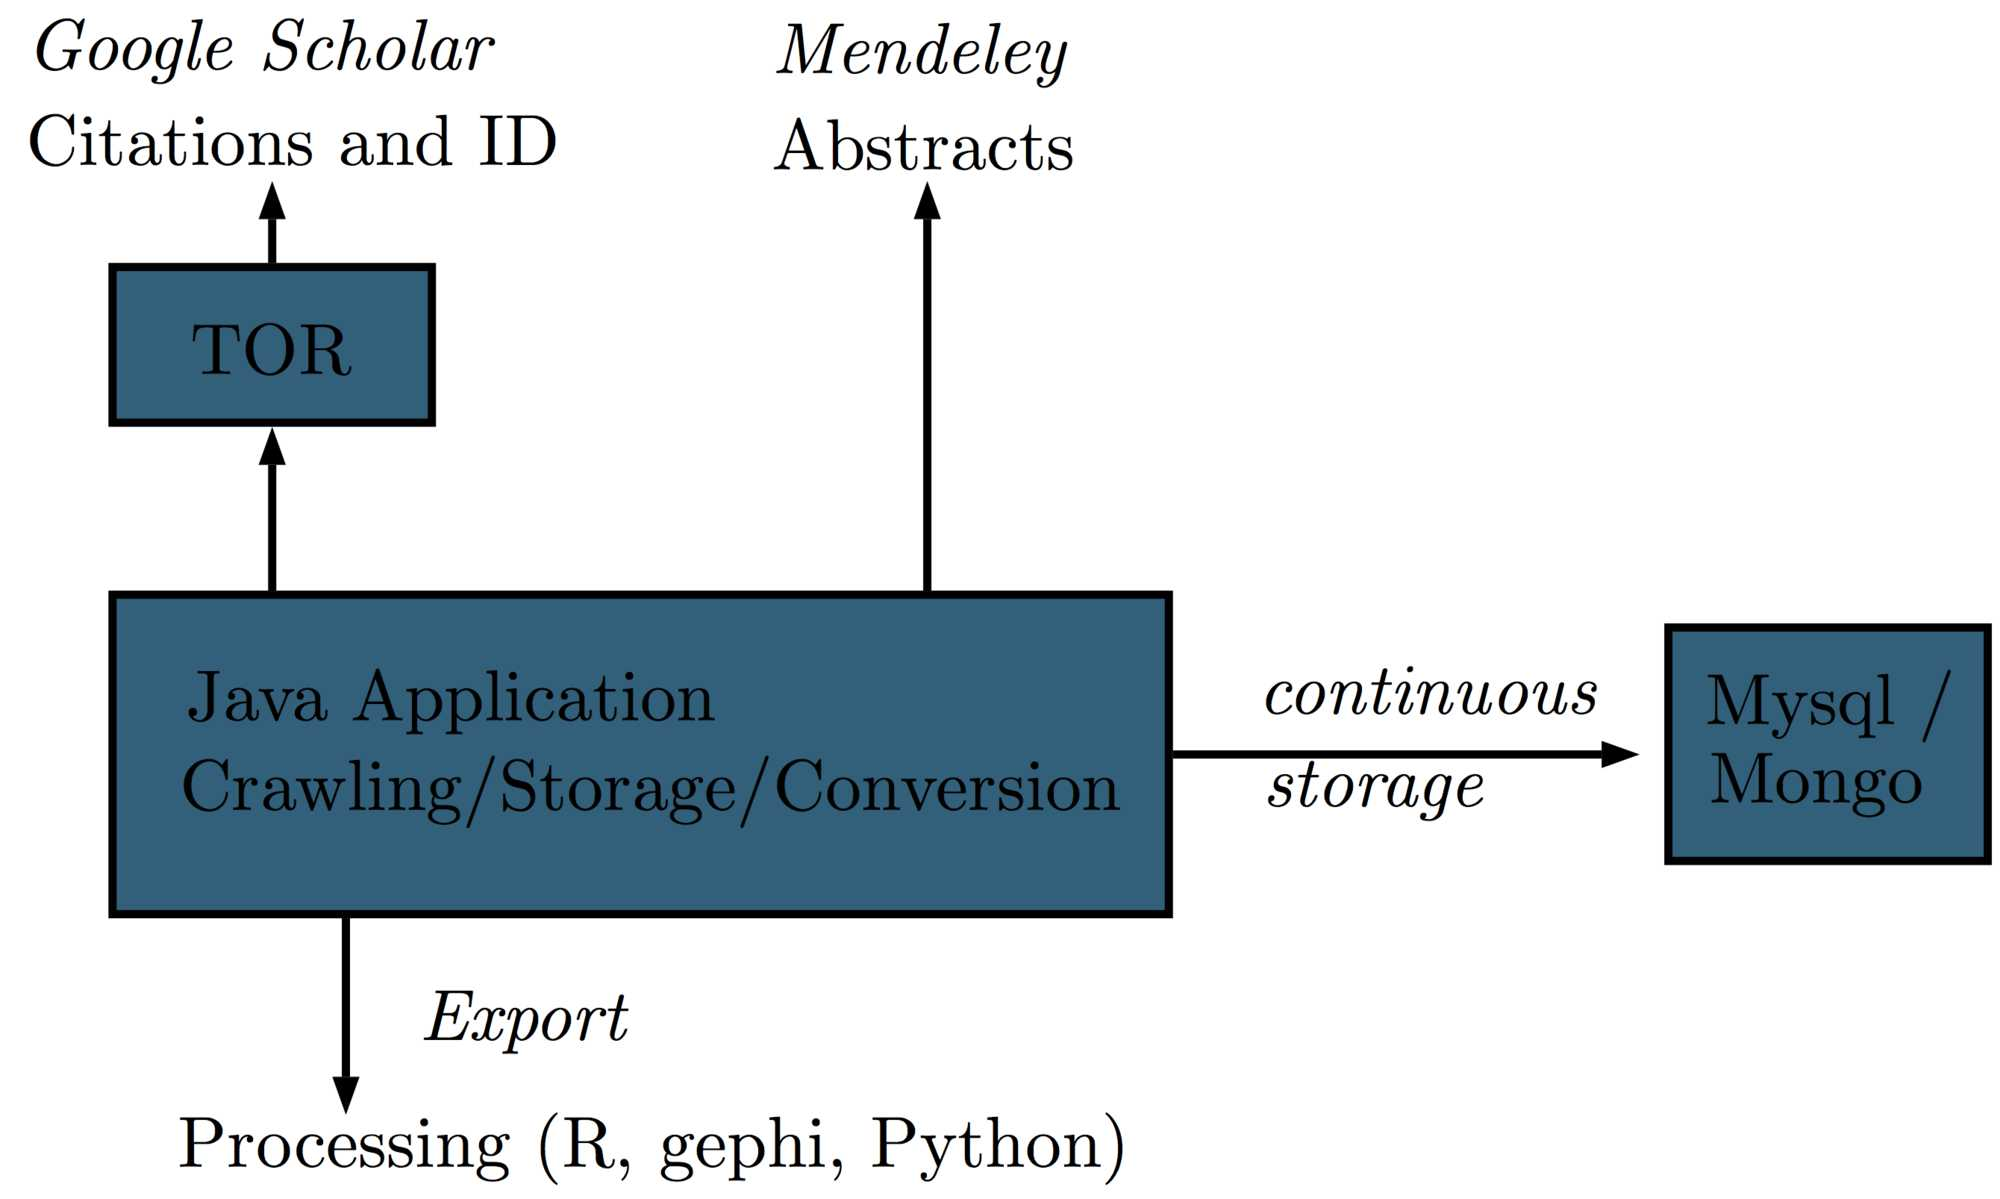
\includegraphics[width=0.7\textwidth]{figures/scim_Fig1.jpg}

}

\sframe{Dataset}{



Citation network with abstract coverage: $\simeq 2.1\cdot 10^5$ papers

\bigskip

\centering

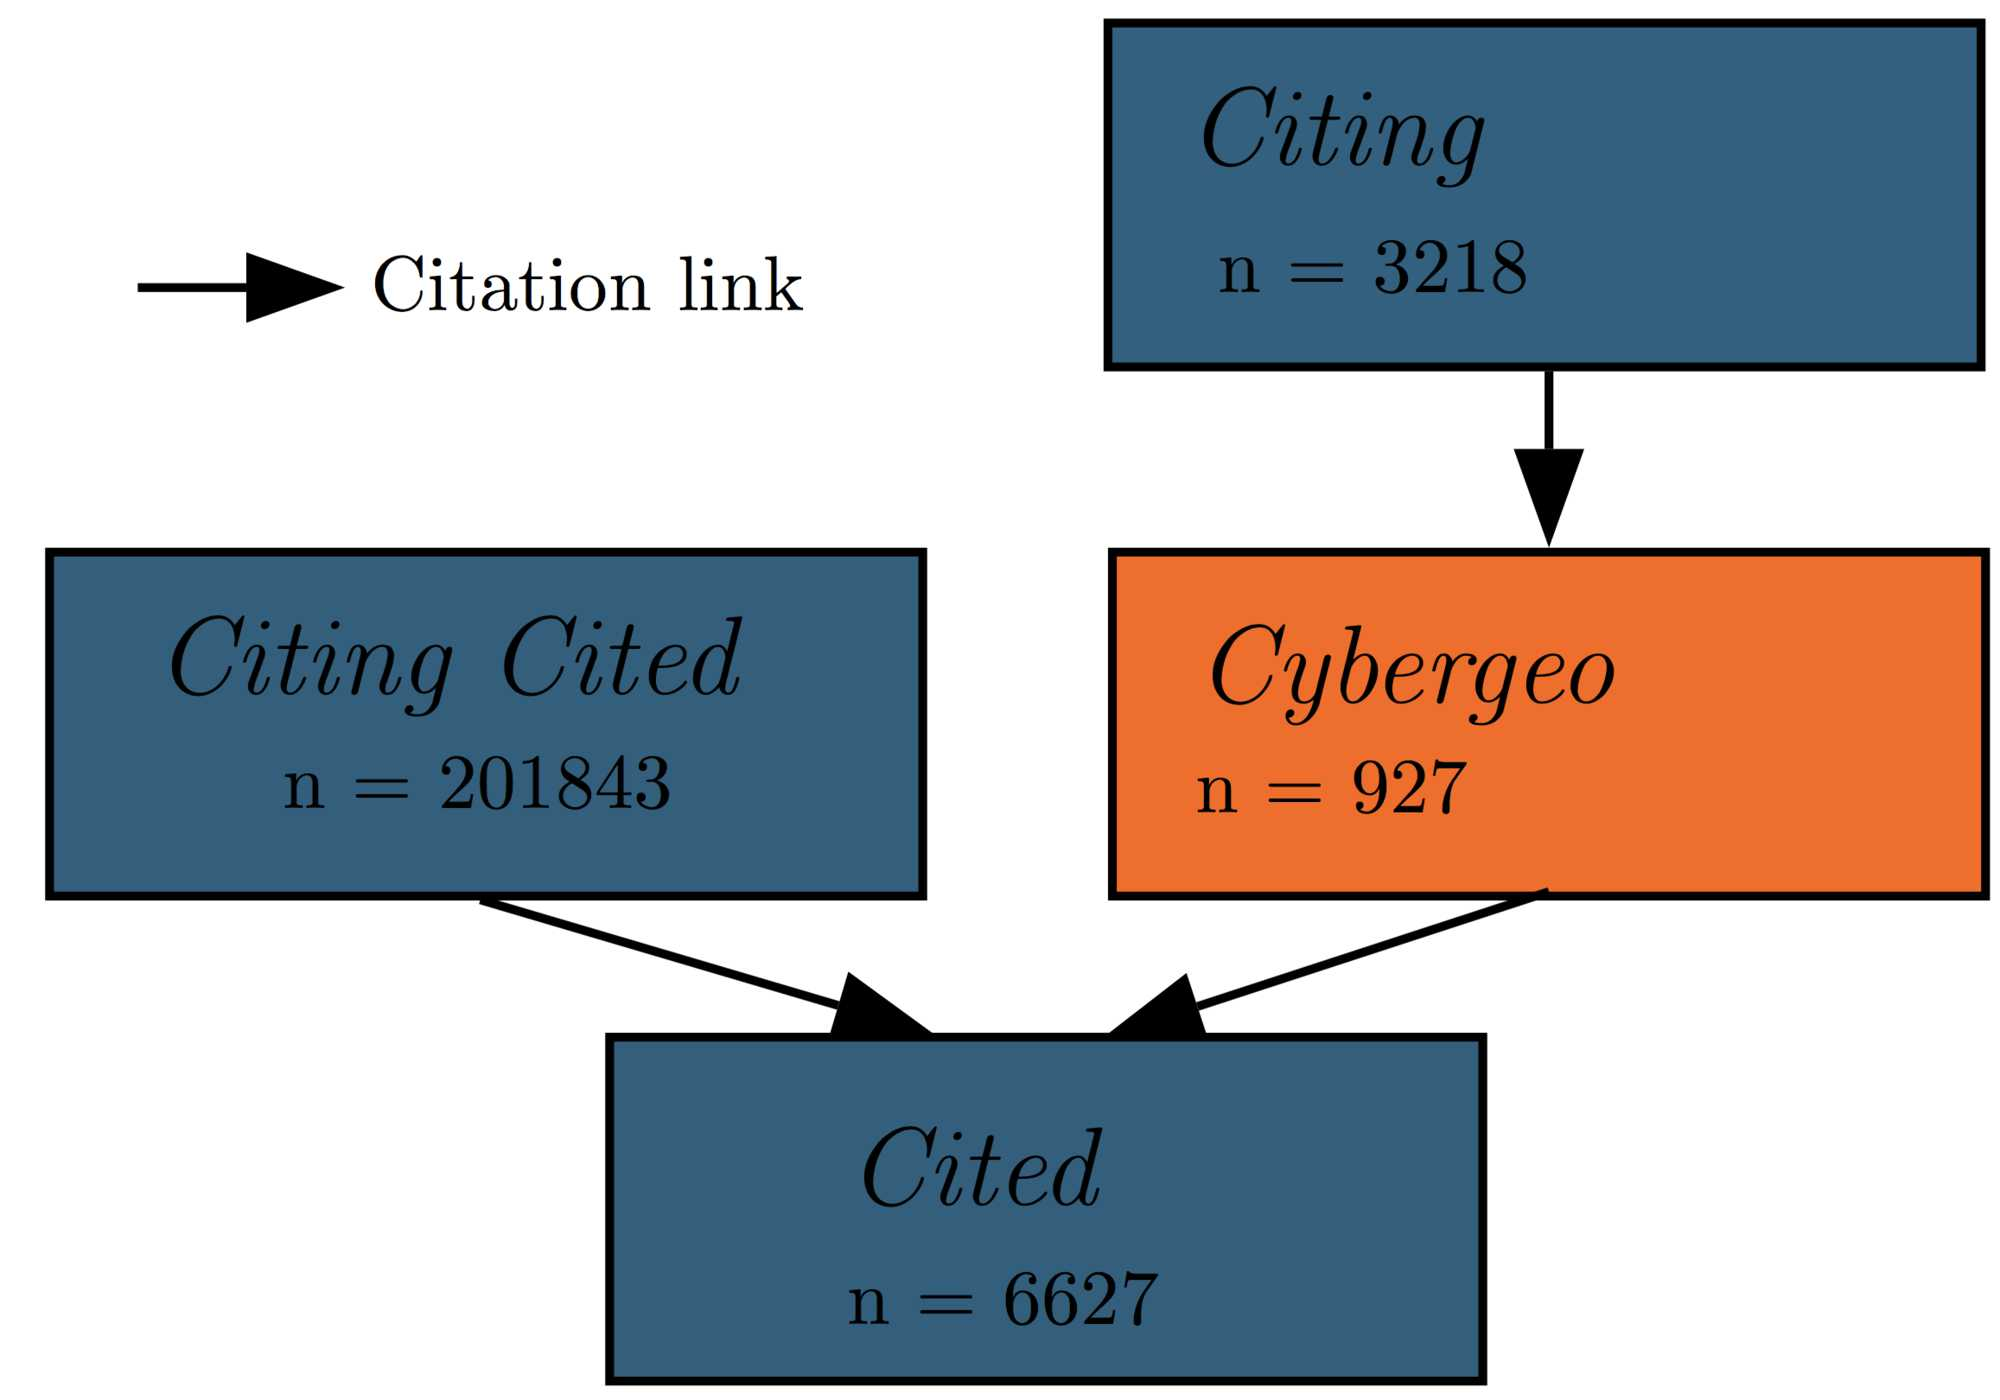
\includegraphics[width=0.7\linewidth]{figures/scim_Fig2.jpg}

}




\sframe{Citation network properties}{



\centering

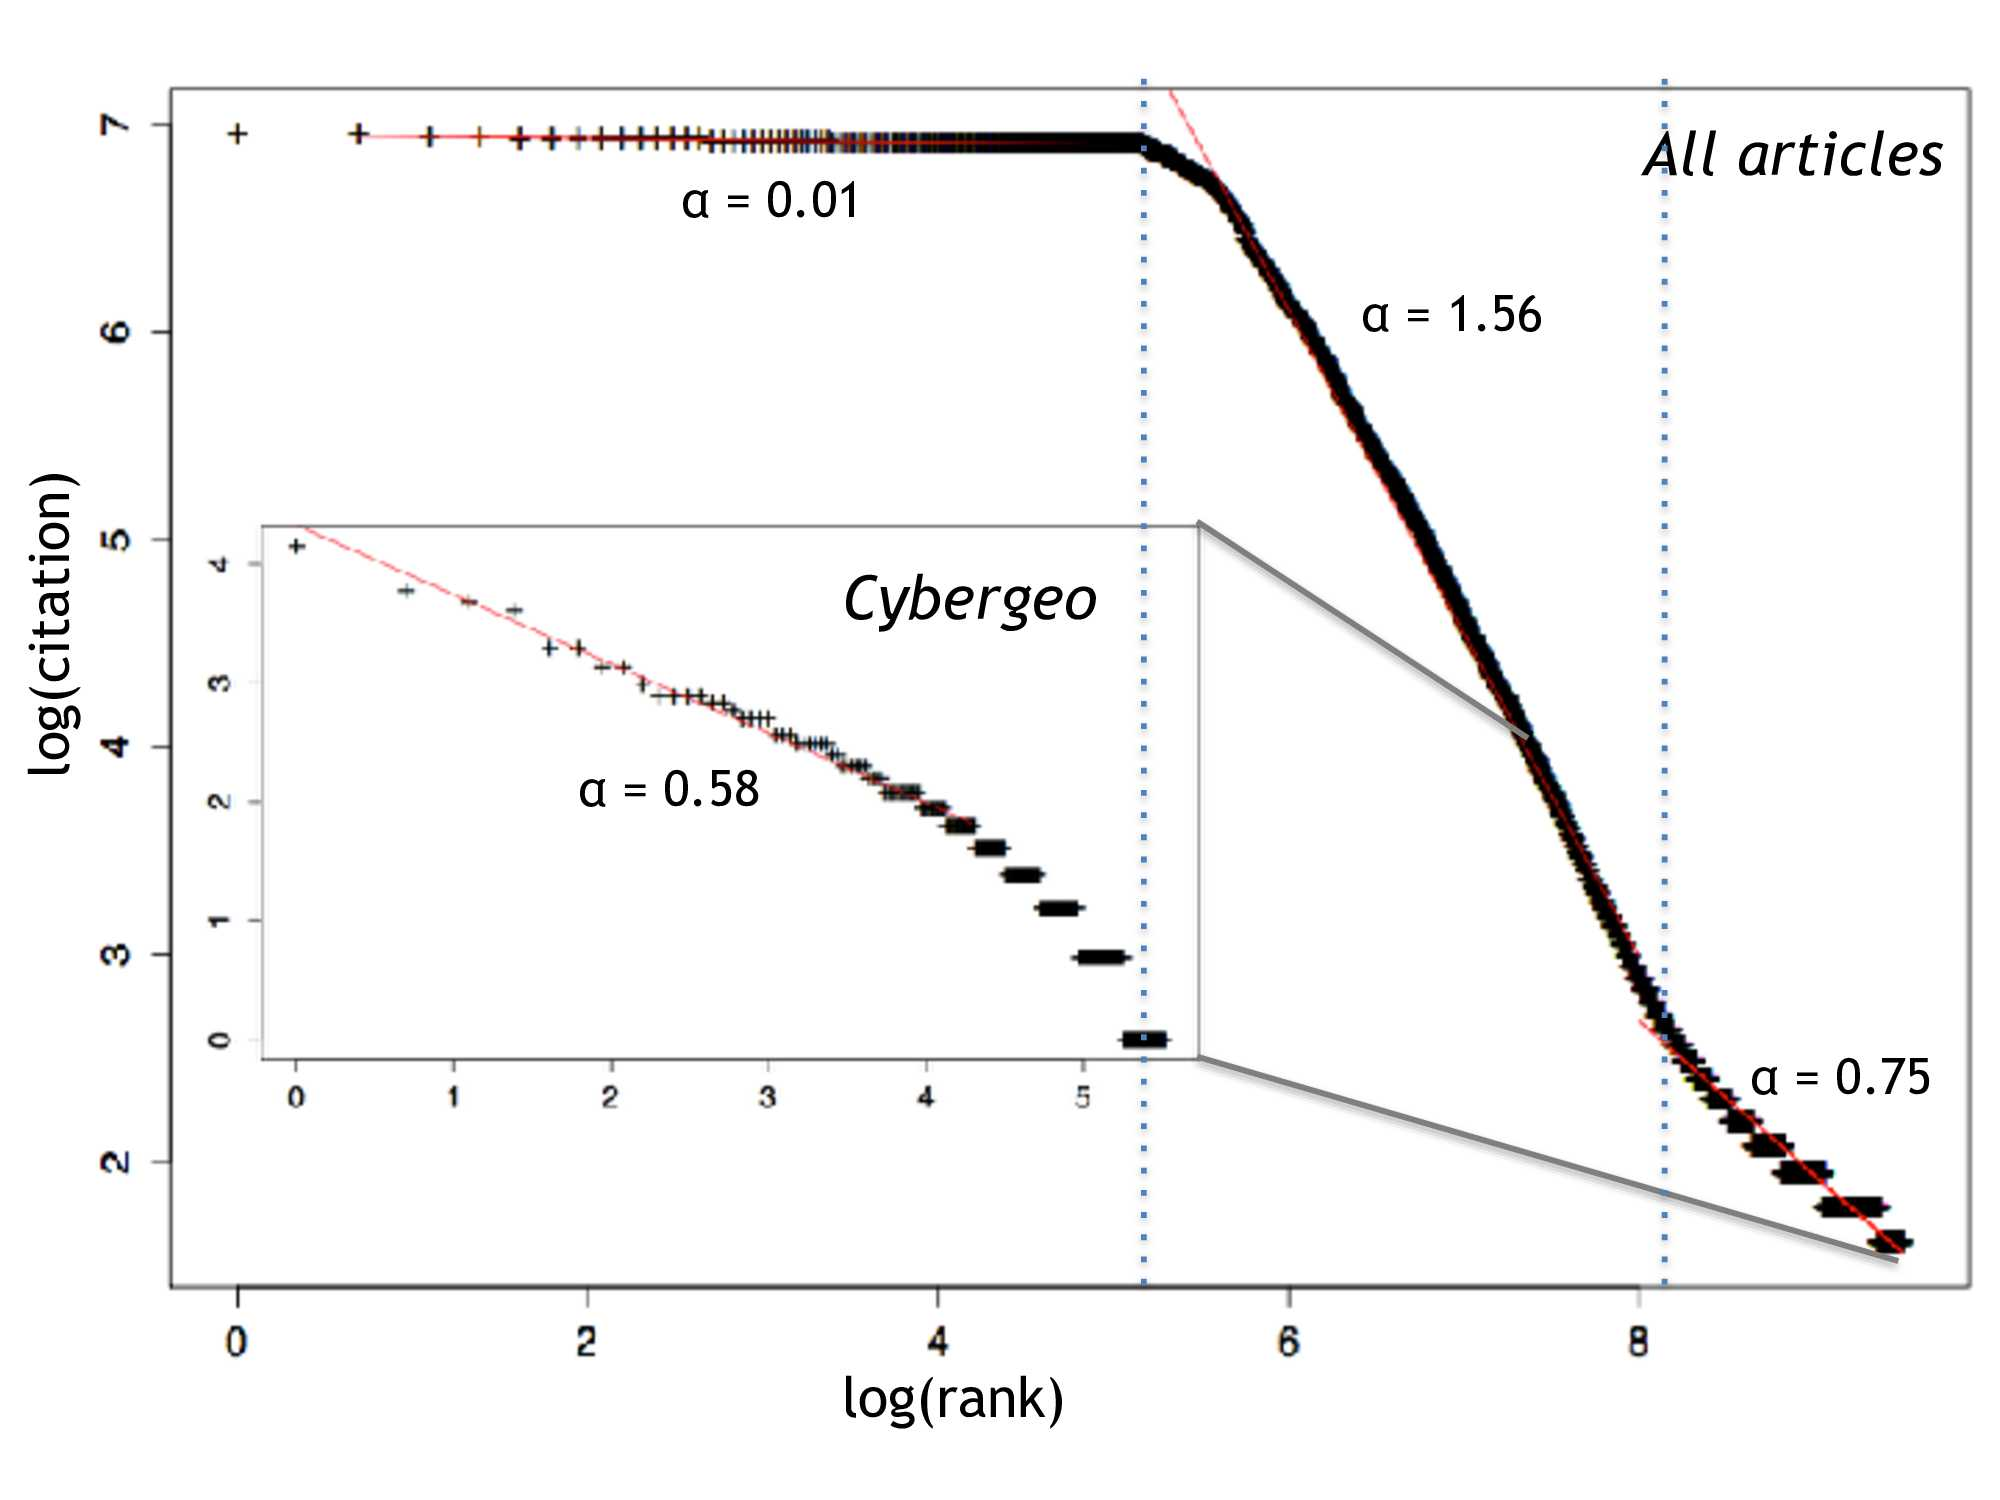
\includegraphics[width=0.9\textwidth]{figures/scim_Fig3.jpg}

}

\sframe{Citation network properties}{

% Other topological properties reveal typical patterns of citation practices, as for example the existence of high-order cliques. Cliques are subset of nodes between which all pos- sible connections exist. Their existence implies citation practices in which all previous papers are systematically cited in new works. The compatibility of this process with the cumulative nature of knowledge may be questionable (Pumain 2005), since the previous knowledge production process is reconstructed each time instead on relying only on the most recent state of knowledge. An exemple of such a clique in shown in Fig. 4, where 6 publications studying the fractal nature of urban structures all cite the previous publica- tions in the clique.

\textit{Example of the largest citation clique}

\centering

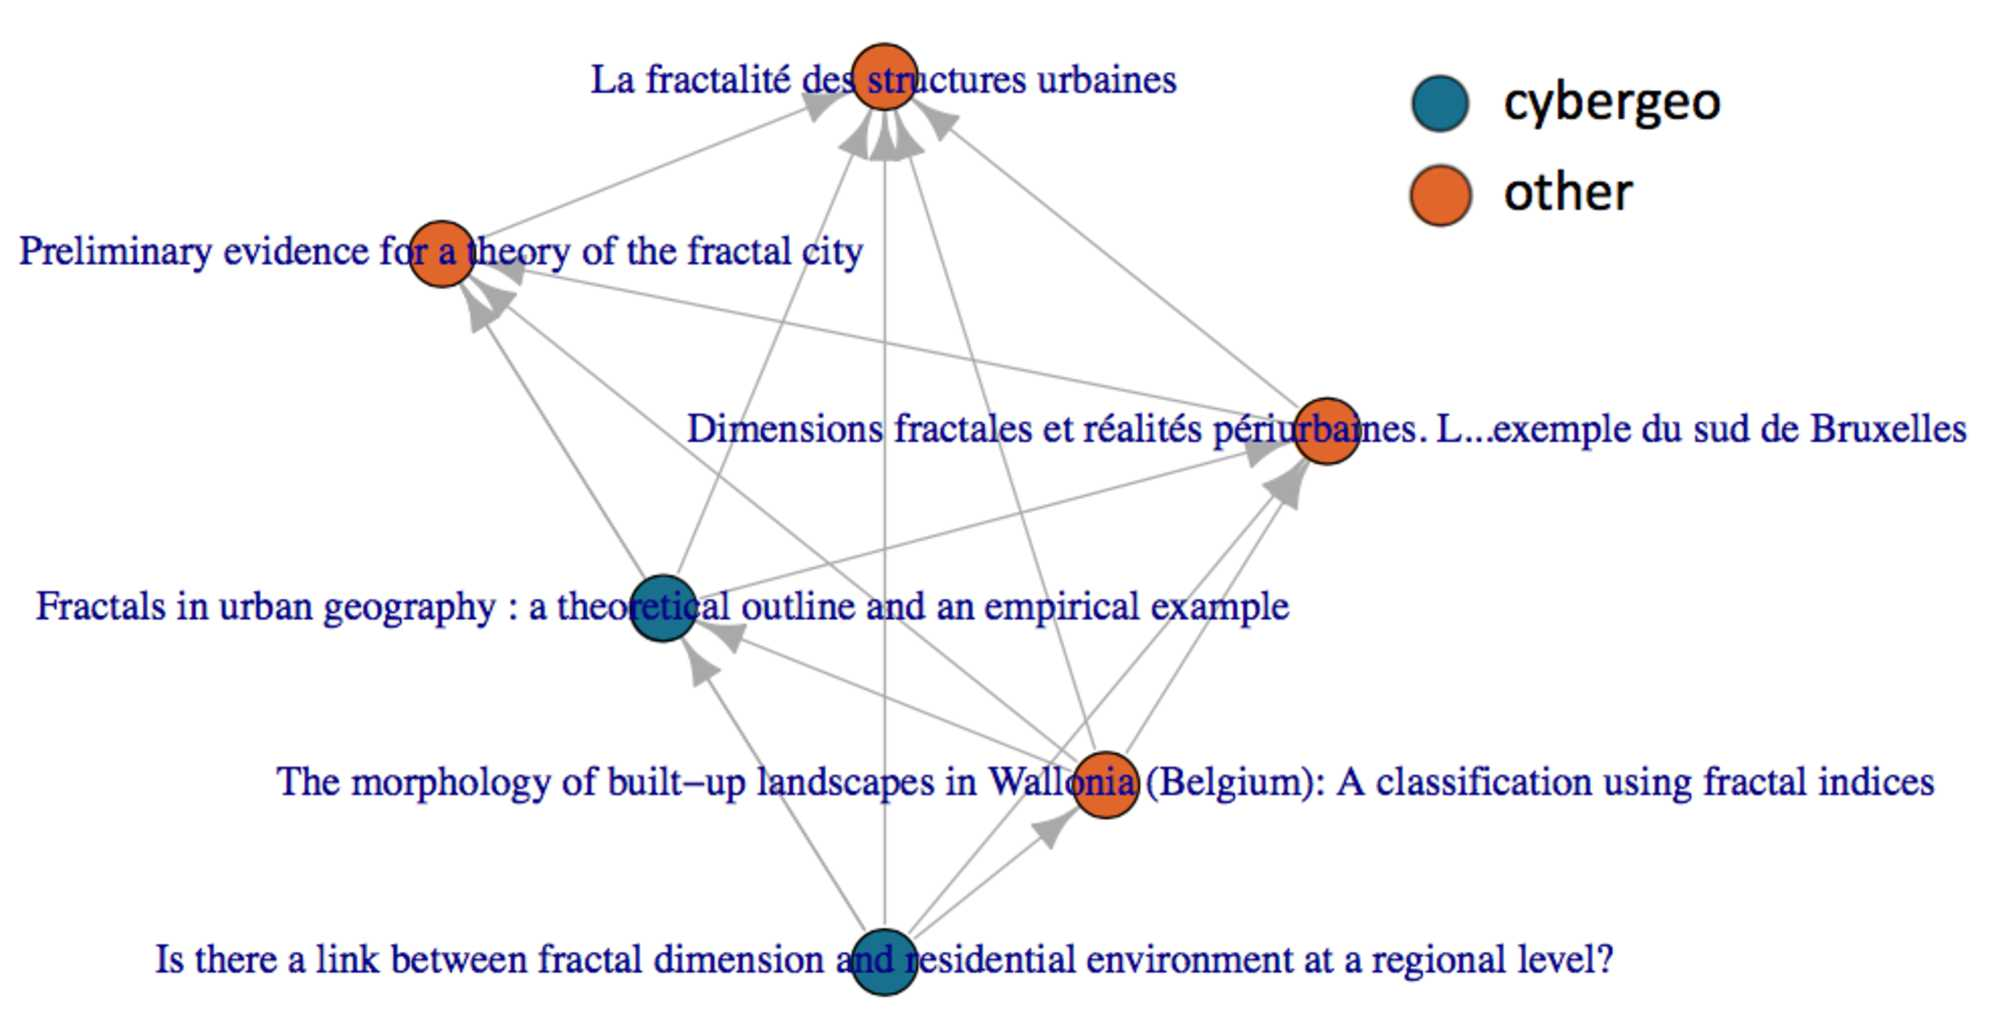
\includegraphics[width=\textwidth]{figures/scim_Fig4.jpg}

}

\sframe{Citation communities}{

% The citation network is a first opportunity to construct endogenous disciplines, by extracting citation communities. More precisely, this step aims at finding recurrent pat- terns in citations that would define a field by its citation practices. In order to be con- sistent with the particular data structure we have (missing incoming citations for sub- corpuses at maximal depth), we filter the network by removing all nodes with degree smaller than one. This ensures that the nodes kept are either at least cited by an other node (and thus there are no missing edges for these nodes) or cite at least two other nodes, what can make “bridges” between sub-communities. The resulting network has a size of |V| = 107,164 nodes and |E| = 309,778 edges. The citation network is visualized in Fig. 5. We use a standard modularity optimization algorithm to identify communities (Blon- del et al. 2008) in the citation network. This Louvain algorithm is applied on the cor- responding undirected network following the elementary solution for community detec- tion in directed networks (Malliaros and Vazirgiannis 2013). It provides 29 communities with a modularity of 0.71, which means that communities are highly integrated [gener- ally, values above 0.4 are already considered as strongly clustered (Newman 2006)]. In comparison, a bootstrap of 100 randomisations of links in the network gives an average modularity of −1.0 × 10−4 ± 4.4 × 10−4. This bootstrap gives statistical significance to the value we obtained, as the observed modularity is larger by more than four order of magnitude than the standard deviation of this null model. We name the communities by inspection of the titles of most cited references in each. This naming process was done under the supervision of the editorial head of the jour- nal. The 14 communities that have a size larger than 2.5% of the network are: Complex Networks, Ecology, Social Geography, Sociology, GIS, Spatial Analysis, Agent-based Modeling and Simulation (ABMS), Socio-ecology, Urban Networks, Urban Simulation, Urban Studies, Economic Geography, Accessibility/Land-use, Time Geography. These categories do not directly correspond to well-defined disciplines, as some correspond more to methods (ABMS), objects of study (Urban Studies), or paradigms (Complex Networks). Some are “specializations” of others: most papers in Urban Studies can also be classified as Critical and Social geography. This way, we construct endogenous disciplines that correspond to scientific practices (what is cited) more than their repre- sentation (the “official” disciplines). The relative positioning of communities in Fig. 5, obtained with a Force-Atlas algorithm, tells a lot about their respective relations: for example, social geography makes a bridge between Urban Studies and Economic Geog- raphy, whereas the connection between Socio-ecology and Urban simulations is done by GIS (what can be expected as geomatics is an interdisciplinary field). GIS also separates and connects two subfield of Ecology, on one side more thematic studies on ecologi- cal habitats, and on the other sides statistical methods. These relations already inform qualitatively patterns of interdisciplinarity, in the sense of integration measures. We will also in the following use these communities to situate the semantic classification.
%Regarding the validity of the map we obtained, the content and structure of our data- set does not allow us to give an exogenous validation using existing techniques Boyack et al. (2005). We rely for the validity of our approach (1) first on the expert knowl- edge used to name the communities; (2) secondly on the high values of the modularity which witness a strong endogenous relevance; (3) the fact that we do not aim to produce exhaustive maps of the discipline, but only to explore the neighborhood of the origin journal; and (4) the low sensitivity to network perturbations as it is developed below in the sensitivity analysis section.


\begin{center}
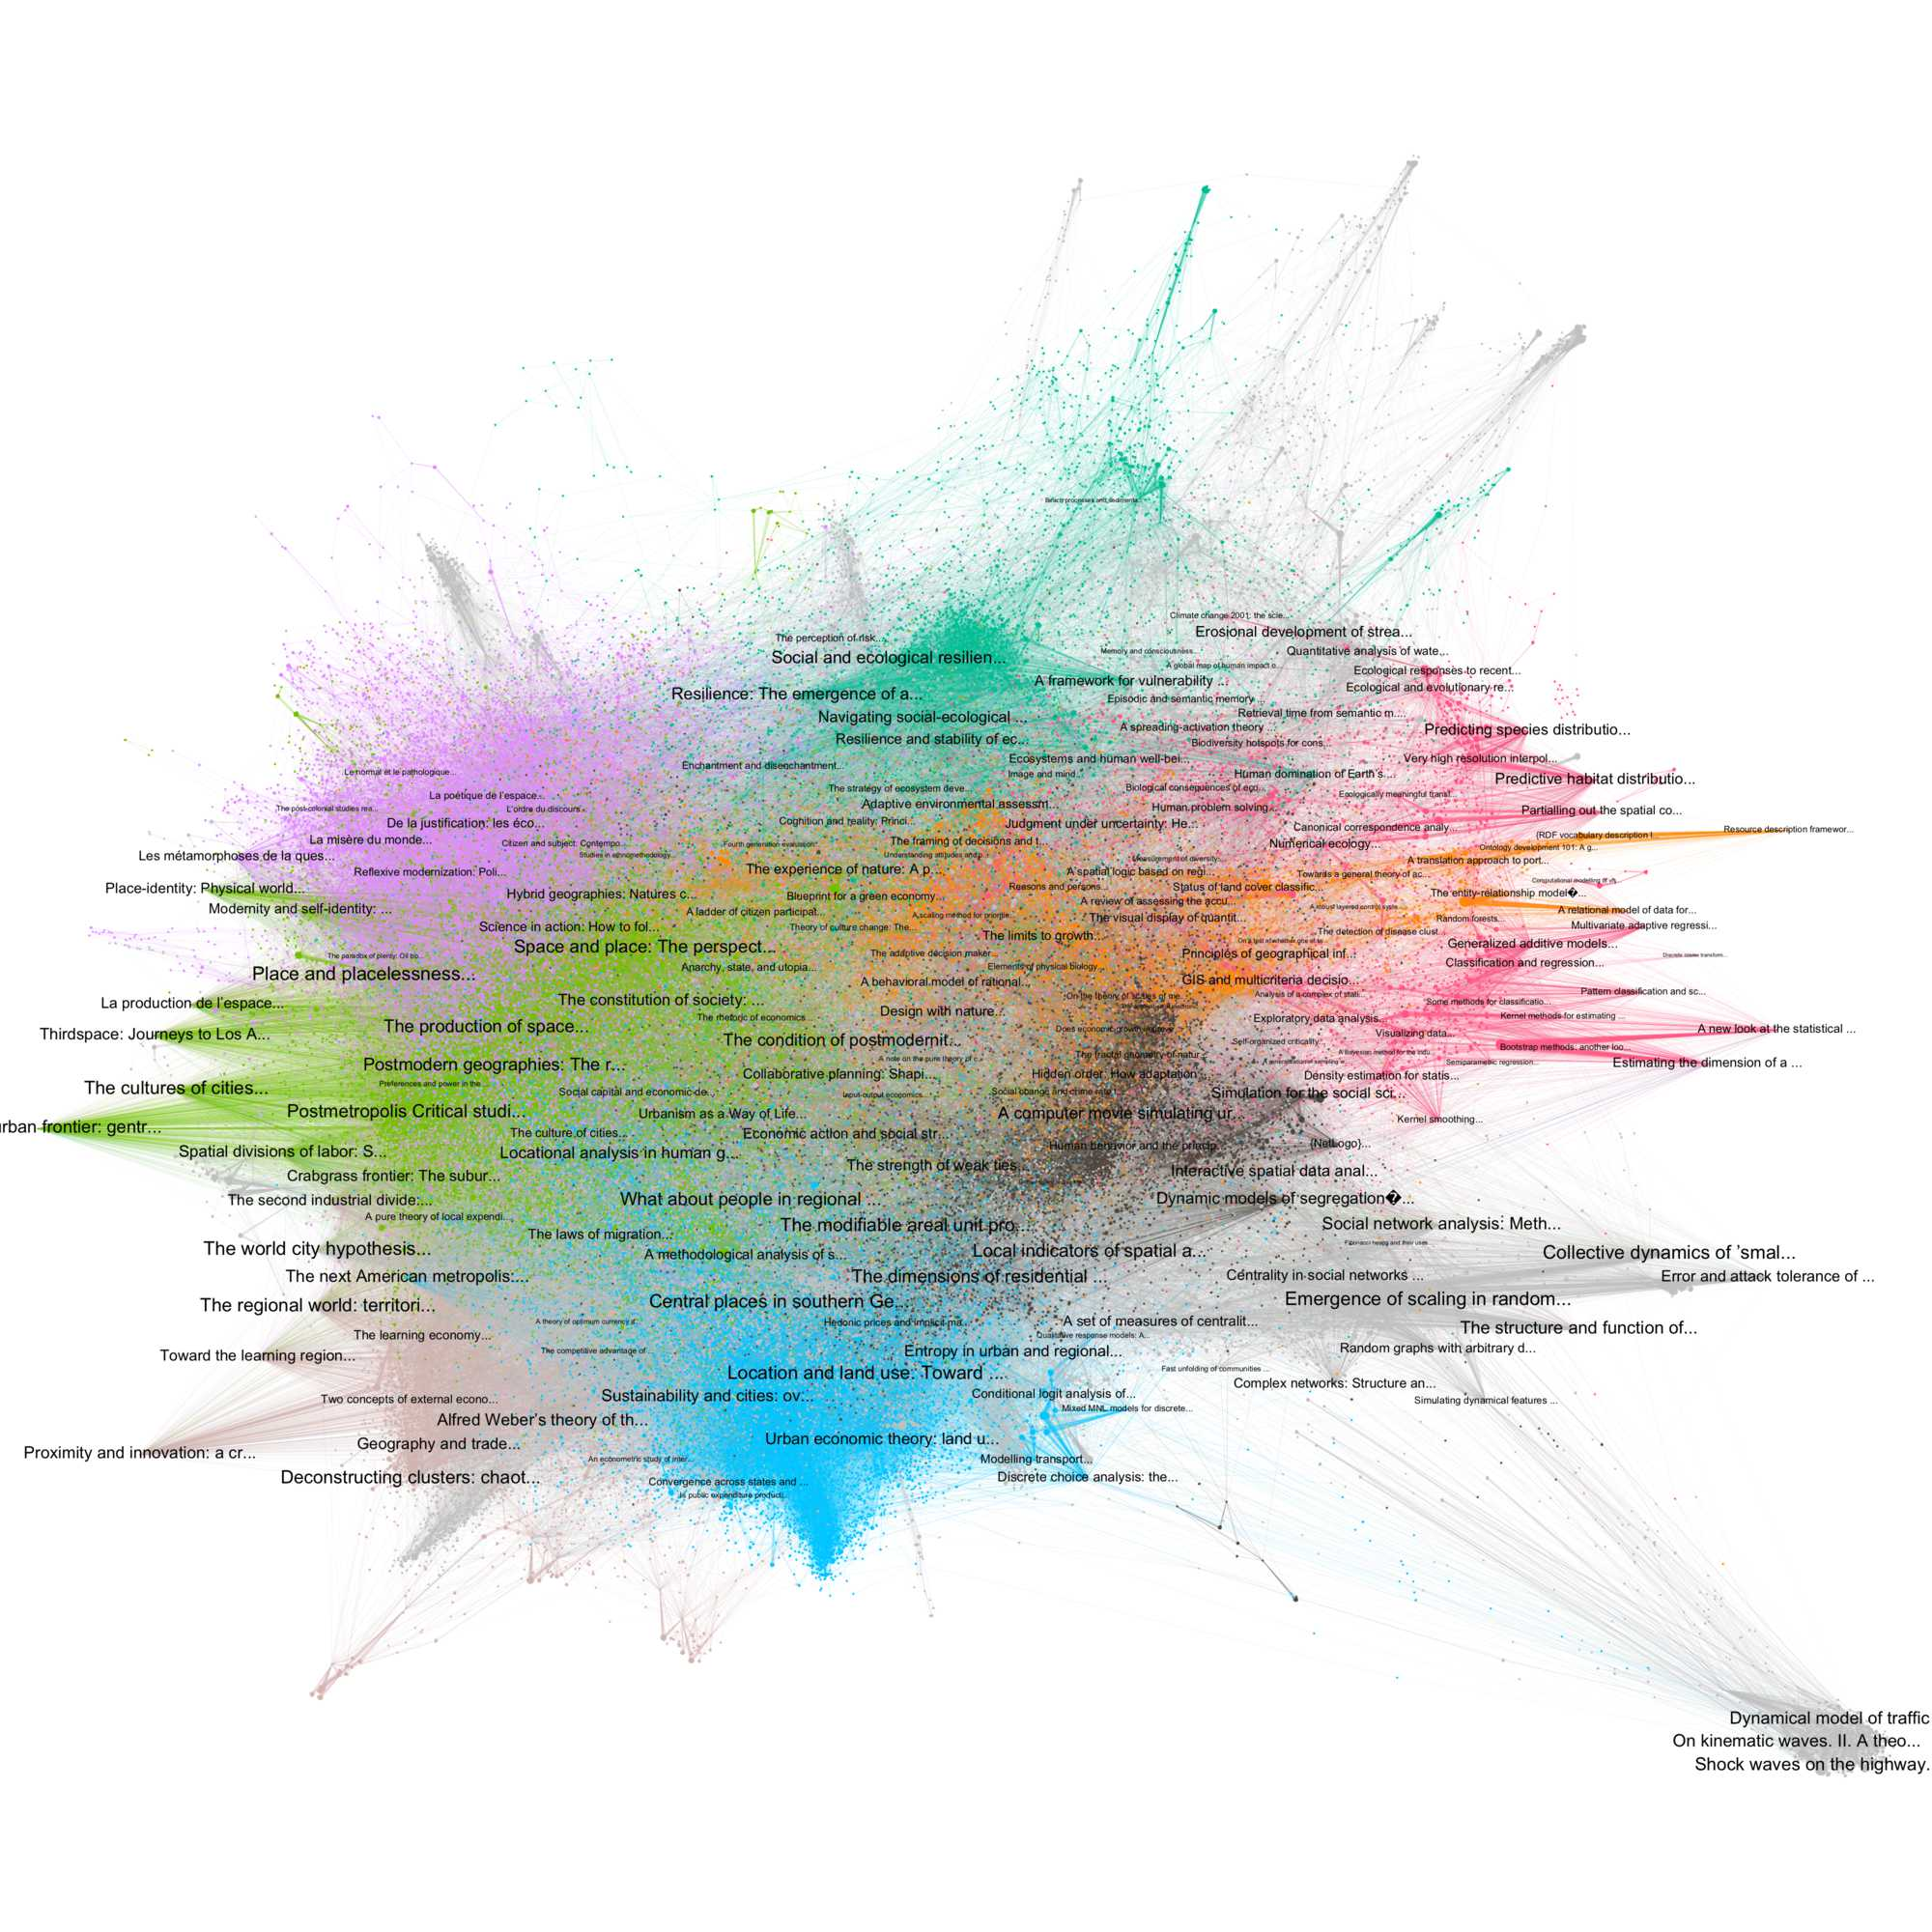
\includegraphics[width=\textwidth,height=0.7\textheight,trim=0 0 0 2cm]{figures/scim_Fig5.jpg}
\end{center}

\footnotesize
\textit{Louvain algorithm community detection to construct endogenous citation communities (modularity of 0.71)}

}


\sframe{Semantic network}{

% We now turn to the methodological details for the construction of the semantic clas- sification. This step adapts the methodology described by Bergeaud et al. (2017), who construct a semantic classification on patent data. We recall that our corpus with available text consists of around 2 × 105 abstracts of pub- lications at a topological distance shorter than 2 from the journal Cybergeo in the cita- tion network. The first important step is to extract relevant keywords from abstracts. Text processing is done with the python library nltk (Bird 2006). We add a particular treat- ment to the method of Bergeaud et al. (2017), as our corpus is multilingual: language detection is done with the technique of stop-words (Baldwin and Lui 2010). We also use a specific tagger (the function allowing the attribution of grammatical function to words), TreeTagger (Schmid 1994), for languages other than English. To summarize, the keyword extraction workflow goes through the following steps:Language detection is done using stop-words, by selecting the language which nltk stop-words dictionary has the most words in common with the current text. 2. Pos-tagging (detection of word functions) and stemming (extraction of the stem) are done differently depending on language: – English: nltk built-in pos-tagger, combined to a PorterStemmer – French or other: use of TreeTagger (Schmid 1994) 3. Selection of potential n-grams (keywords of length n with 1 ≤ n ≤ 4) following the given grammatical rules to identify noun phrases: for English⋂{NN ∪ VBG ∪ JJ}(which cor- respond respectively to noun, gerund verb, adjective), and for French ⋂{NOM ∪ ADJ} (respectively noun, adjective). More elaborated procedures to infer grammatical rules for noun phrases by learning from corpuses do exist (Cardie and Pierce 1998), but are devised to gain knowledge on grammar specifically. We follow the simple procedure of Chavalarias and Cointet (2013) with these simple fixed rules for noun phrases, similarly to Kumar and Srinathan (2008) without the use of heavy additional dictionaries for filtering. Other languages are a negligible proportion of the corpus and are discarded. 4. Estimation of the relevance n-grams, by attributing a score following the deviation of the statistical distribution of co-occurrences to a random distribution. 
% We keep at this stage a fixed number KW of n-grams, based on their relevance score, that will be designated as the relevant keywords. We find that for large values of KW , results are not sensitive to the total number of keywords, and take a reasonably large value for com- putational performance, KW = 50, 000. We construct the co-occurrence matrix of the rel- evant keywords. This co-occurrence matrix provides the semantic network as its adjacency matrix: nodes are keywords, and they are linked according to their co-occurrences.

Construction of the semantic network as a co-occurence network between keywords extracted following \cite{bergeaud2017classifying}:

\medskip

\begin{enumerate}
	\item Language detection using stop-words \cite{baldwin2010language}
	\item Part-Of-Speech tagging (\texttt{nltk} or \texttt{TreeTagger} \cite{schmid1994probabilistic}); stemming
	\item Construction of potential n-grams: nouns and adjectives up to size 4
	\item Estimation of n-gram relevance following the deviation to the expected statistical distribution of co-occurences (chi-squared test)
\end{enumerate}



}

\sframe{Sensitivity analysis of the semantic network}{

% We observe the same phenomenon than in Bergeaud et al. (2017), that is the existence of nodes with large degree and not specific to a particular field: for example model and space are used in most of subfields of Geography. We also adapt the original filtering procedure, as we do not have here an exogenous information to calibrate parameters. We assume the highest degree terms do not carry specific information on particular classes and can be thus filtered given a maximal degree threshold kmax. We keep the second filter on a minimal edge weight threshold 𝜃 . We add the supplementary constraint that keywords are also filtered on a document frequency window fmin,fmax (number of references in which they appear), what is slightly different from network filtering. A sensitivity analysis of resulting network topology to these four parameters is presented in Fig. 6. Given a filtered network, we detect communities using modularity optimization as before for the citation network. Various properties of the network can be optimized, and we look in particular at its size (number of keywords after filtering), the optimal modularity, the number of communities, and the balance between their sizes (defined as a concenration index This multi-objective optimization problem does not have a kk kk unique solution as objectives are contradictory in a complex way, and a compromise point must be chosen. Indeed, one can obtain a very high modularity but with a small network which will finally cover only a small fraction of the corpus, whereas a large network yields lower modularity values as shown in Fig. 6. The process is similar for other indicators. We take a compromise point between modularity and network size, with a high balance and a reasonable number of communities, given by kmax=1200,𝜃w=100,fmin=50,fmax=10000. This point was taken on the com- promise line between modularity and network size (roughly around the line link- ing (𝜃w = 50, kmax = 400) with (𝜃w = 100, kmax = 1200)), with a high balance (taking kmax ≥ 1000) and not too much communities. These values give a network of size 2868, with 18 communities and a modularity of 0.57. Note that the small proportion of keywords in French is always separated from the rest of the network as they cannot co-occur with English keywords, and that with these param- eter settings no French keywords are kept. All communities described in the following therefore contain only keywords in English.

\justify

\vspace{-0.5cm}
Additional filtering procedure to remove relevant but common keywords: filter on edge weight and maximal degree; values chosen based on multiples objectives including modularity and network size.

\medskip

\centering

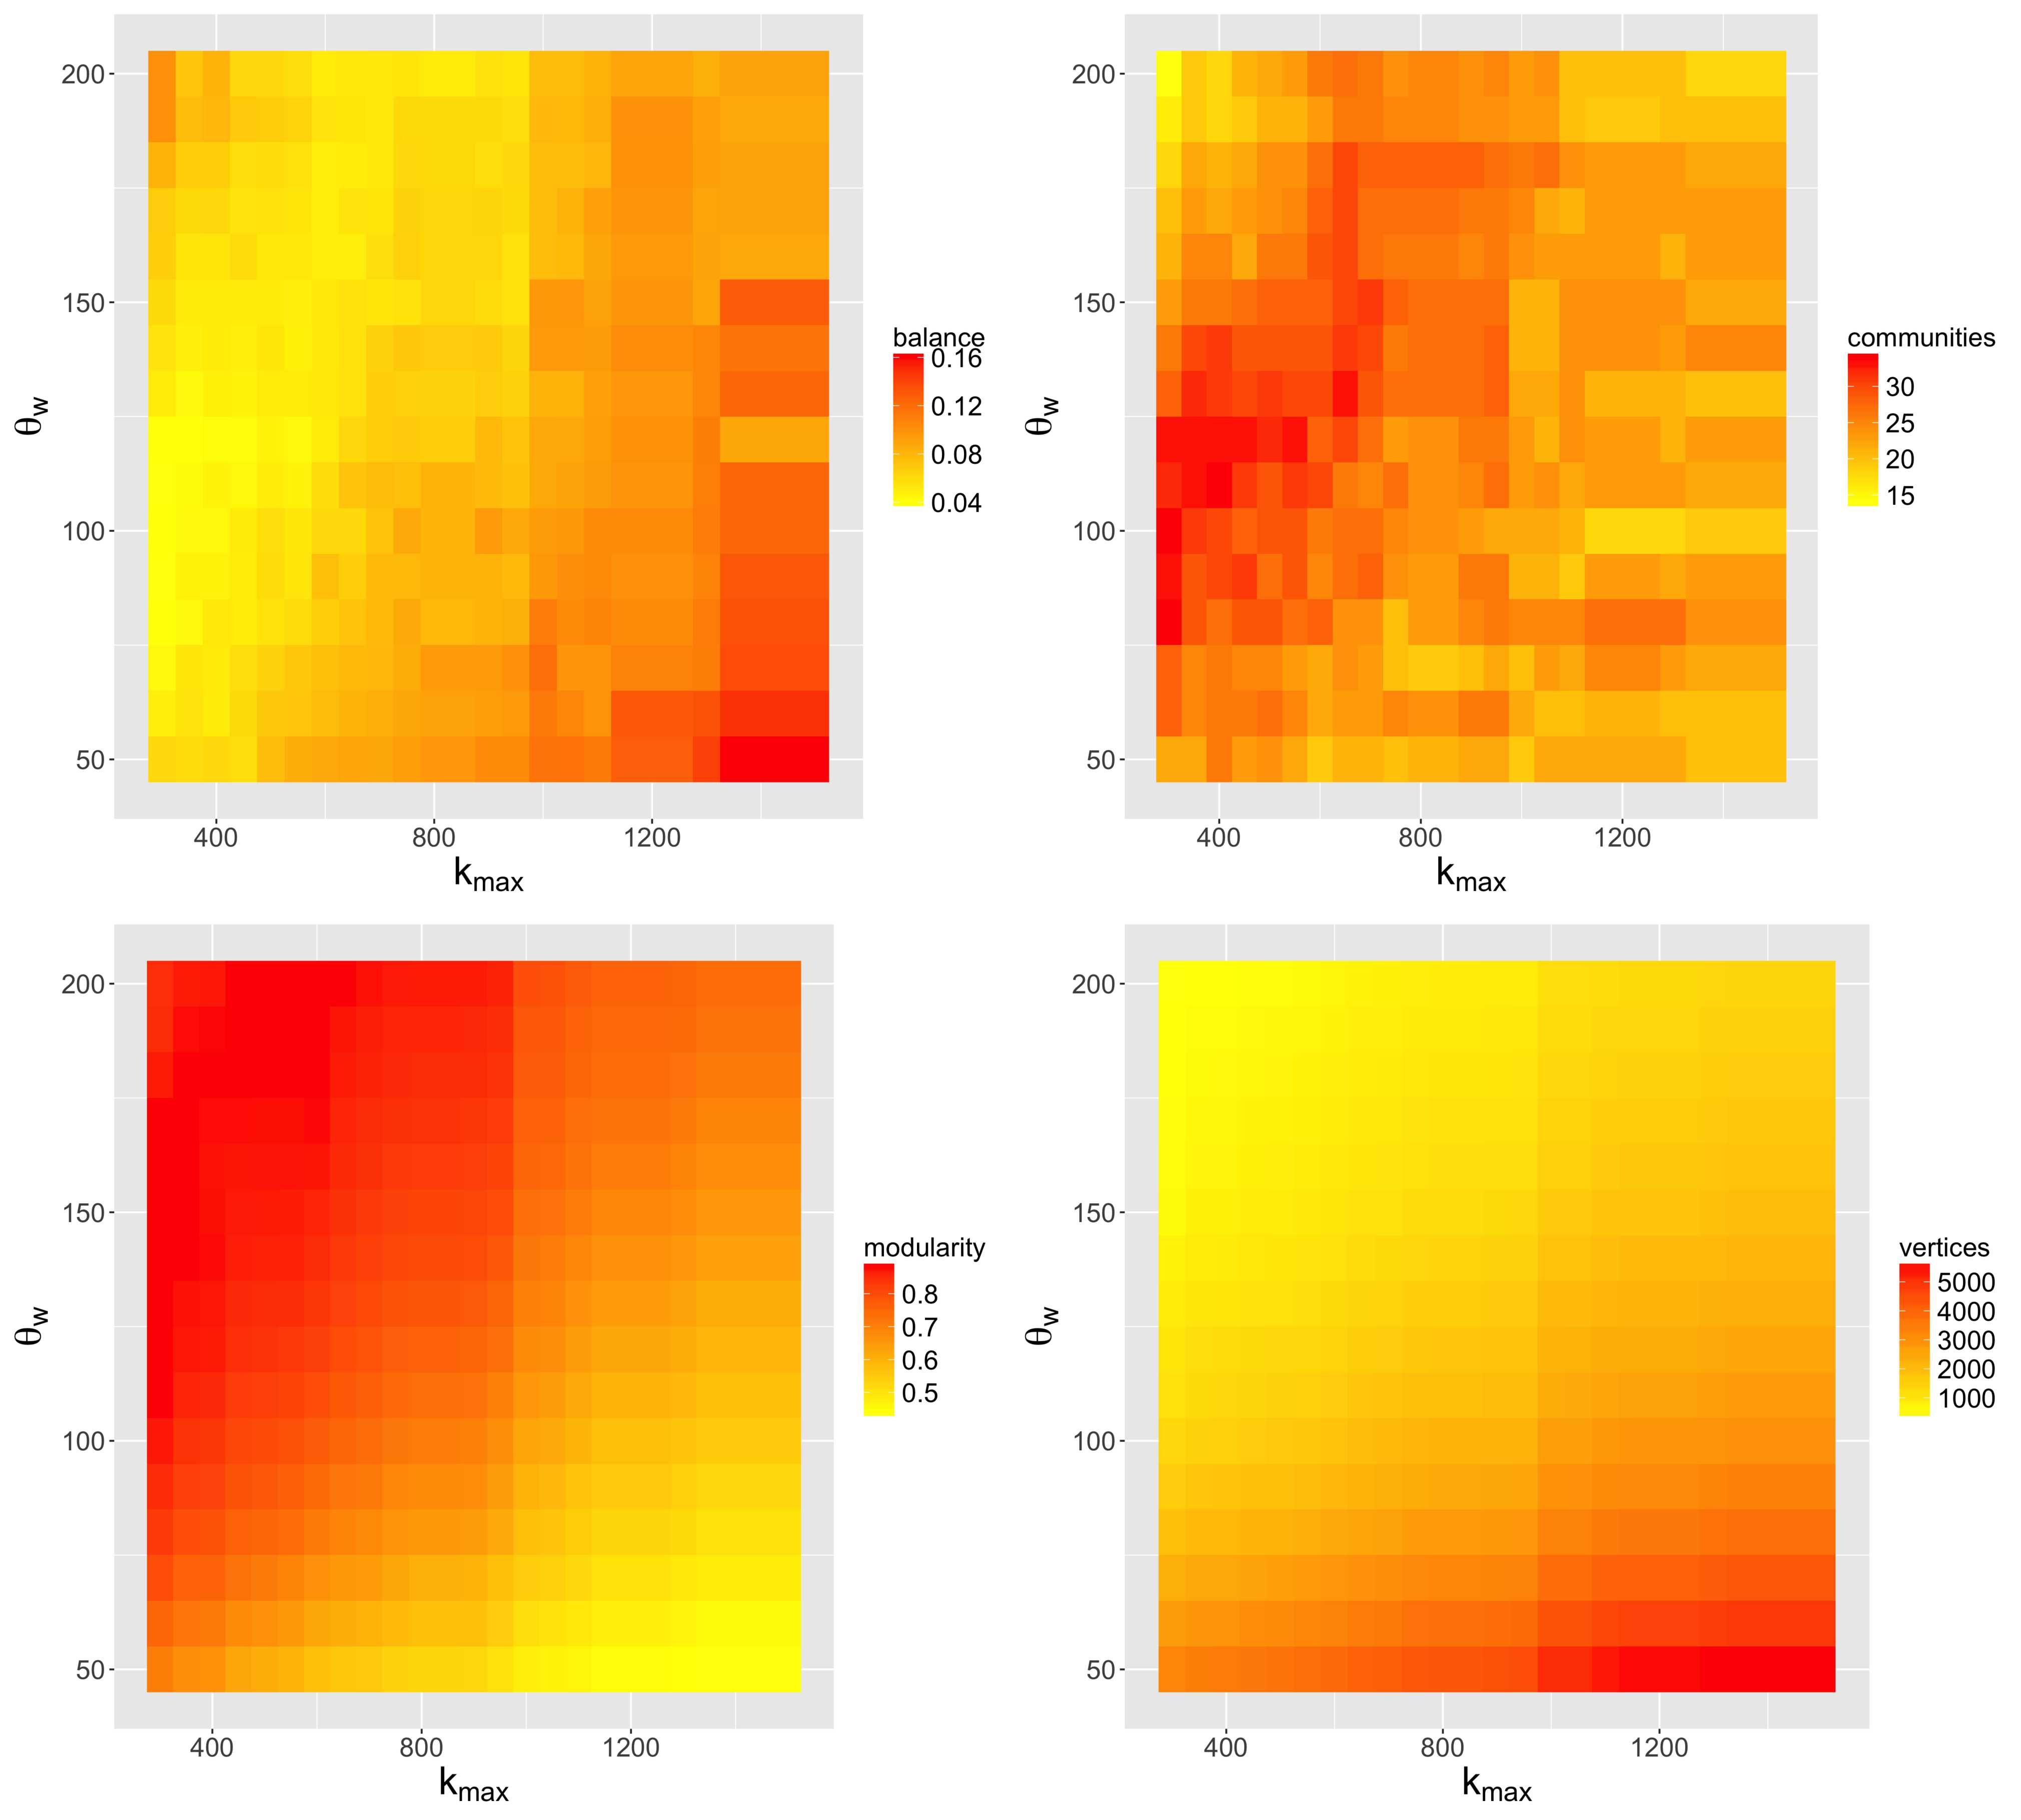
\includegraphics[width=0.6\textwidth]{figures/scim_Fig6.jpg}

}

\sframe{Semantic network visualization}{

\centering

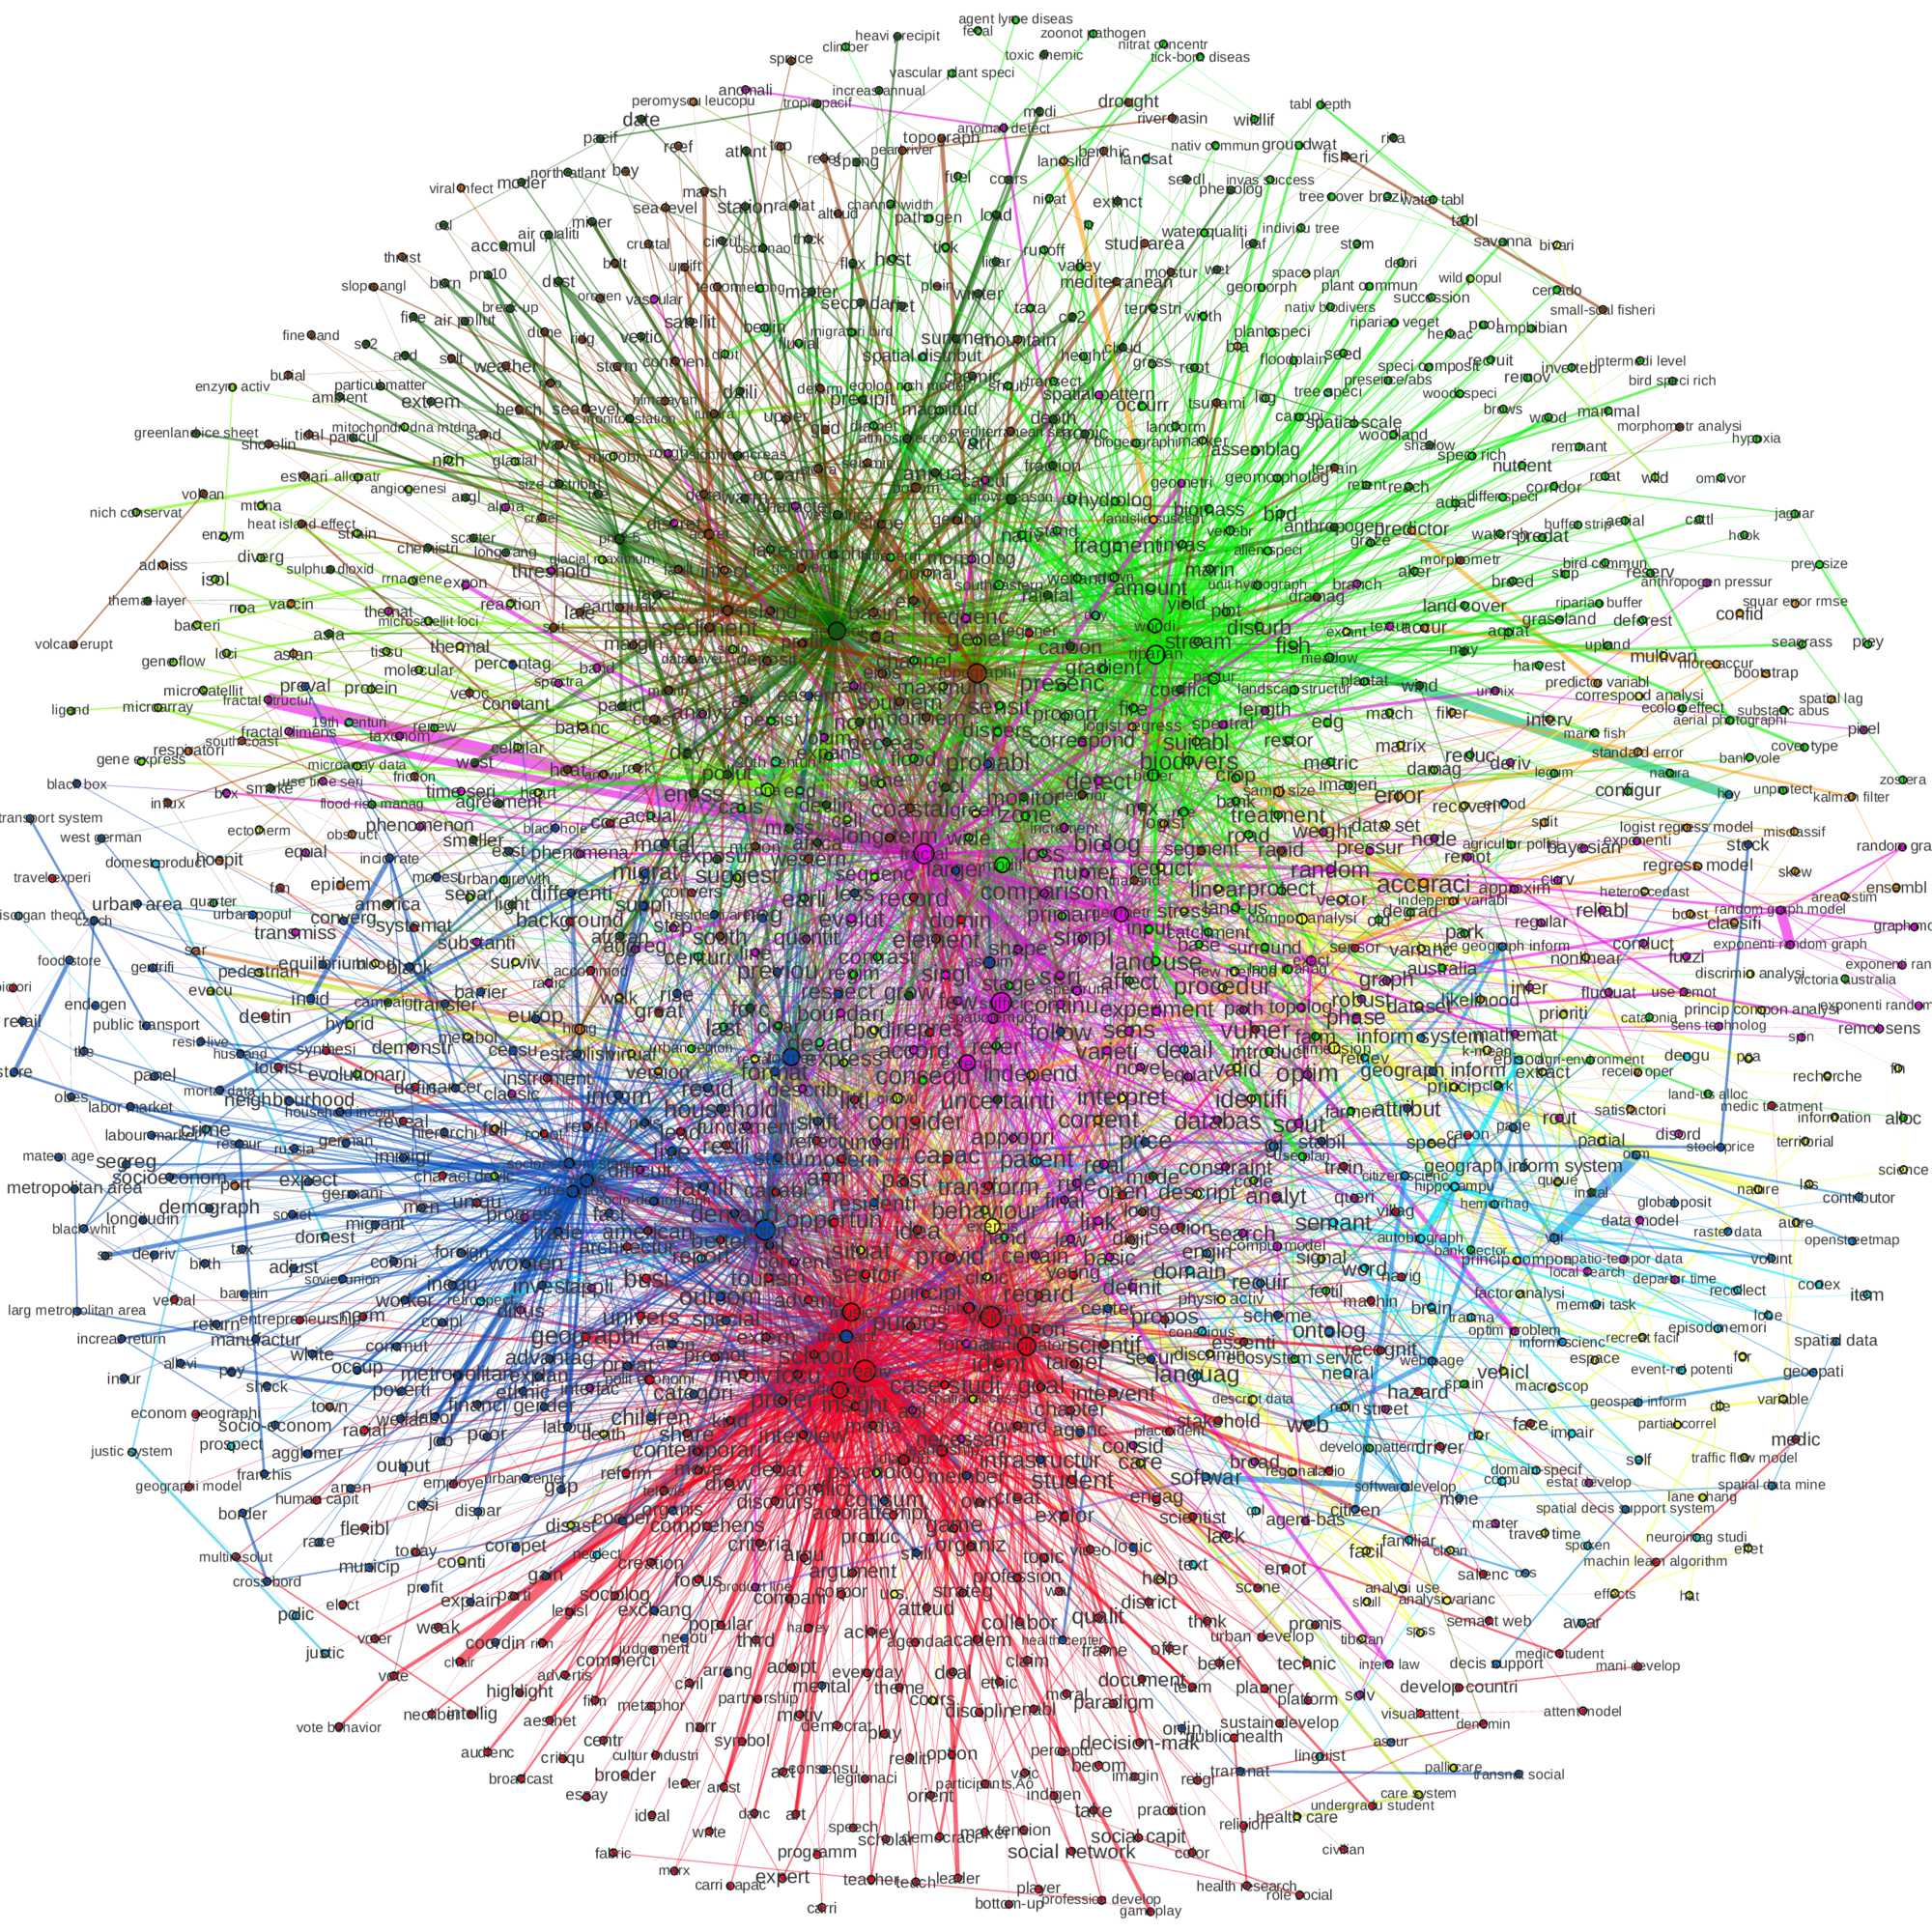
\includegraphics[height=0.9\textheight]{figures/scim_Fig7.jpg}

}



\sframe{Semantic communities}{

% We obtain therein communities in the semantic network with the optimized filtering param- eters. At the exception of a small proportion apparently resulting from noise (representing less than 10 keywords in 3 communities that we remove, i.e. 0.33% of keywords), commu- nities correspond to well-defined scientific fields, domains, or approaches. Naming is also done by inspection of the most relevant keywords in each community, in order to stick here to a certain level of supervision. Table 1 summarizes the communities, giving their names, sizes, and corresponding key- words. The most important community is related to issues in political science and critical geography, what could have been expected as several previously obtained citations commu- nities (Social geography, Urban studies) deal with these issues. We then obtain a large clus- ter of terms related to biogeography, that must correspond to publications in Ecology and Socio-ecology identified before, together with a community in Environment and Climate. In a way similar to the citation communities, but more pronounced here, we obtain endogenous “disciplines” that can correspond to real disciplines, to methodologies, to object of studies. This classification thus also unveil effective scientific practices, here in terms of semantic content. A class here related to complex systems can be associated to a paradigm and various approaches that were separated in the citation communities: agent- based models and complex networks for example. On the contrary, some studies that were gathered in a large domain before can be precisely differentiated in the semantic network, such as microbiology and health here that are used by studies related to socio-ecology or ecology in the citation network. Some very specific domains appear here as they have very few connections in their actual semantic content: for example, Geography of crime is very precise and disconnected from other communities. We show in Fig. 7 a visualisation of the semantic network, in which the positioning of communities, induced by a Fruchterman–Reingold algorithm [that we use here to have a more precise layout in the relative positioning compared to Force Atlas (Jacomy et al. 2014)]. The bridging between distant disciplines is done quite differently compared to the citation network, and reveals thus qualitatively an other dimension of interdisciplinarity, i.e. the semantics shared by disciplines. Here, the communities corresponding to Economic Geography (blue) and to Critical Geography (red) are close as in the citation network, but are linked to ecology and geomorphology (green and brown) by Complex Systems (magenta), although these were not present as a community in the citation network. Com- plexity methodologies such as Fractals, Scaling (West 2017) or Networks (Newman 2003) are indeed widely used both in social sciences and in physics or biology. The semantic analysis reveals thus that very distant disciplines, that are distant in their citation patterns, are finally close in terms of actual content. This conclusion can naturally subject to the bias that similar terms can correspond to very different ontologies in each disciplines. This actual meaning is partly captured in the embedding of the term in the semantic network, and how it relates to other terms in the semantic network. To what extent ontological prox- imities can be associated to semantic proximities or reconstructed from the network struc- ture is an open question out of the scope of this work. Terms must thus not be dissociated from their context, which in our case is given by the citation network, thus the interest of the analysis below on the relation between classifications.

\centering

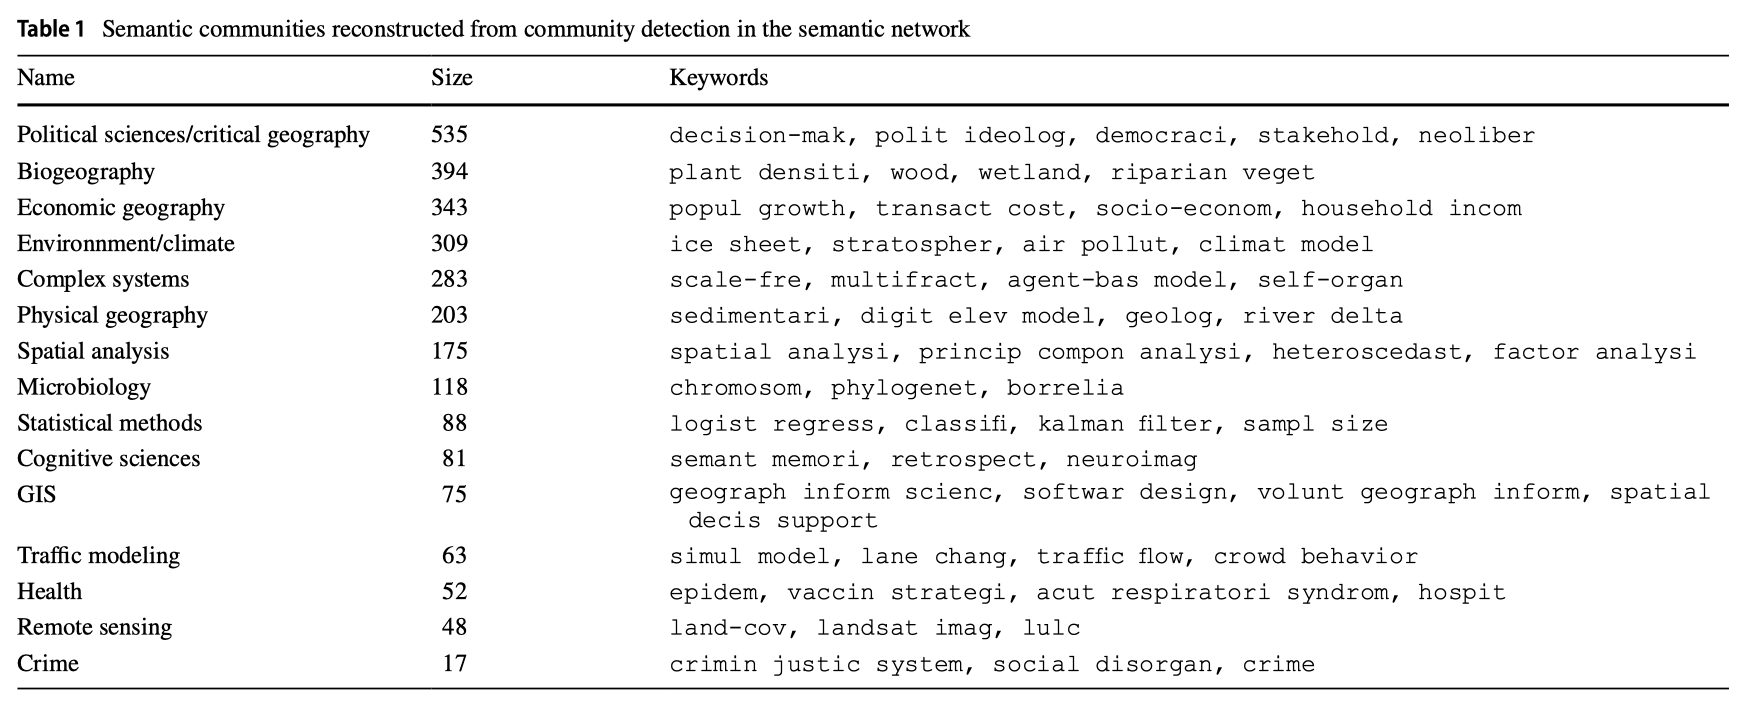
\includegraphics[width=\linewidth]{figures/scim_Tab1.png}

}



\sframe{Interactions between communities}{

% In terms of overlaps between communities, in the sense of co-occurrences of cor- responding keywords within texts of references, we show a synthesis of links between semantic communities in Fig. 8. We see that communities such as Critical Geography and Biogeography are not totally disconnected and share still a certain number of co-occur- rences. More isolated communities can be spotted such as Health and Crime Geographies. Surprisingly, Statistical Methods does not share strong links with other communities, what could mean that articles dealing with methodological issues in this field are rather discon- nected from the field of application, or at least do not describe it extensively. On the con- trary, methods in Complex Systems are organically integrated with the thematic issues they tackle.


\centering

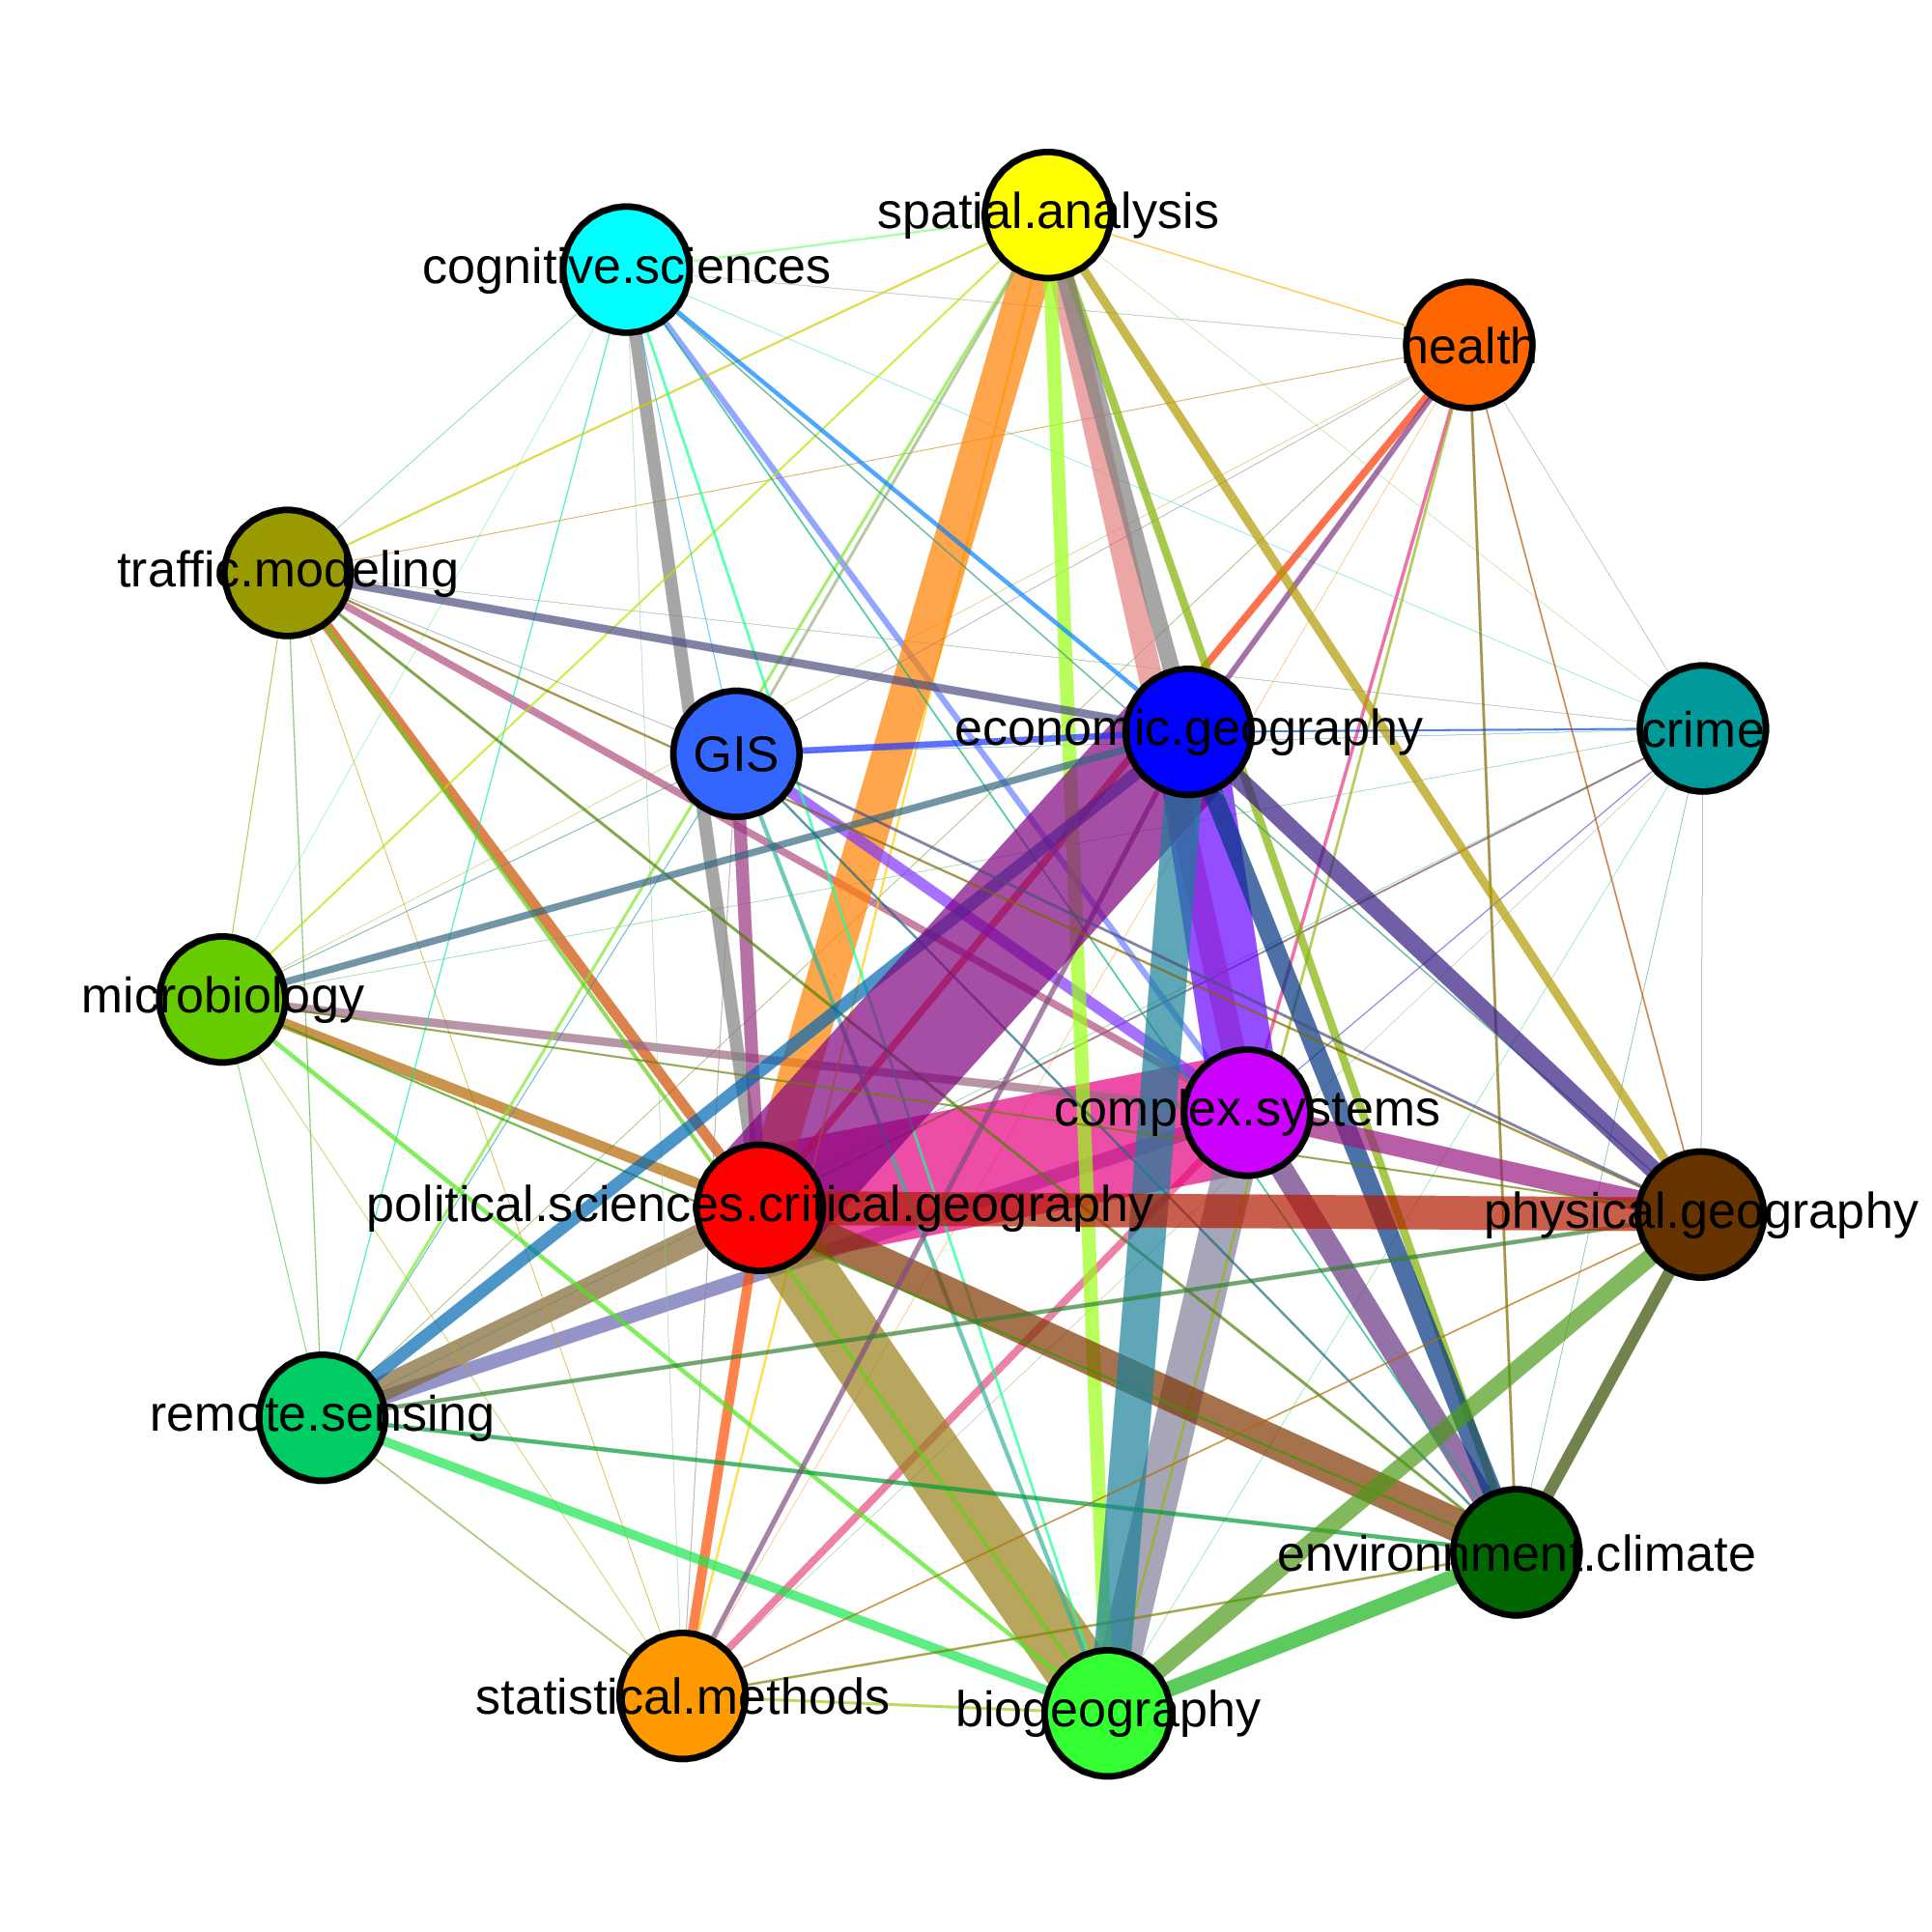
\includegraphics[height=0.9\textheight]{figures/scim_Fig8.jpg}

}


\sframe{Sensitivity to corpus definition}{

% To give a stronger confidence in the results we obtain, we need to study the influence of corpus choice, since (1) our case study is a narrow part of the related disciplines; and (2) the interaction between missing data and the methodology introduced may play a role in the result obtained, that then could be solely due to spurious effects between both. How- ever, our data collection process and classification method were conceived to be used together: using both layers increase the information that can be extracted, since the col- lected data has less information than classical datasets. Our positioning regarding data, i.e. working only with the open dataset in a case of a low data availability, does not allow us to proceed to “ground truth” validations with an exogenous classification. We can however study endogenously the sensitivity of the com- munity structure to the corpus definition, by studying the sensitivity to data removal. This controls the process used by data quality and contributes to the validation of the method, rather independently to the dataset used. The procedure is the following, according to classical approaches to the study of net- work robustness (Trajanovski et al. 2013): working on the citation network, we test the sensitivity of the community structure to entity removal. A fixed proportion r of nodes or edges are removed randomly, and modularity is estimated in the resulting network. This procedure is bootstrapped Nb = 1000 times for each value. Results are shown in Fig. 9, for 0.05 ≤ r ≤ 0.5. We obtain similar qualitative patterns for node and edge removal regarding the form of distributions, but the median modularity slightly decreases for nodes whereas it oscillates for edges. Extreme values are higher for nodes, up to 0.02 difference in absolute value. This remains a very low absolute value, and we find that the community structure has a low sensitivity to data removal, in terms of missing reference (node) or citation link (edge), when going up to 50% of missing data. This gives confidence in the fact that our method is stable relatively independently of the choice of the origin corpus. We also tested the influence of the time window used, since our origin corpus spans between 1996 and 2016. We filter the citation network on fiver-year sliding win- dows covering this span. The size of corresponding subnetworks is relatively stable (|V| ∈ [27866;60474] and |E| ∈ [18839;33892]) and the modularities are higher than the full network (between 0.84 and 0.88) and stable. This suggests that the community struc- ture is stable in time.


\begin{center}
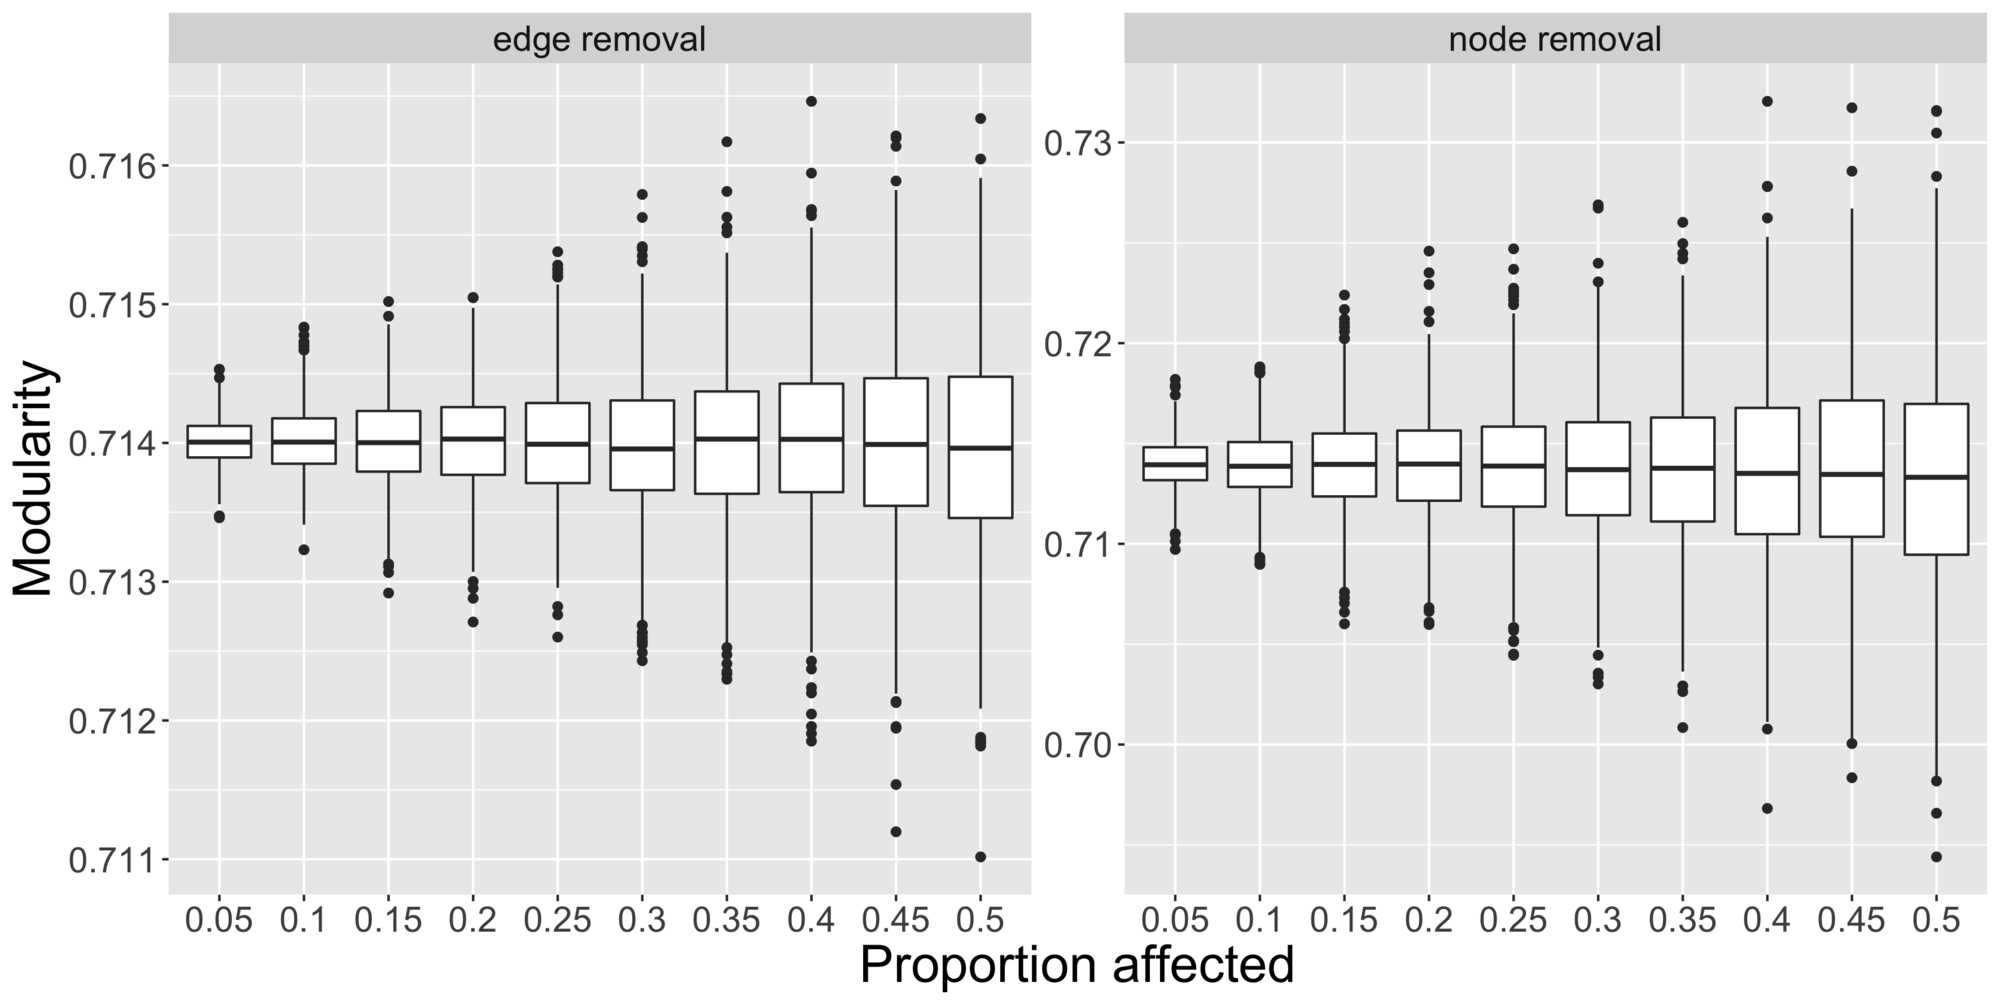
\includegraphics[width=\textwidth]{figures/scim_Fig9.jpg}
\end{center}

\medskip

\textit{Impact of node and edge removal on the optimal modularity of the citation network}


}


\sframe{Semantic composition of citation communities}{

% We can now turn to the study of the relation between classifications. First, a simple way to link them is to look at the semantic content of citation communities. Each reference has a given proportion of keywords within each semantic class, and an average composition in terms of semantic classes for each citation class can thus be computed. We show these composition in Fig. 10. Some expected results are obtained, such as Complex Networks (citation) having the largest part in Complex Systems (semantic), or GIS (citation) the larg- est in GIS (semantic), and similarly for Economic Geography. But the study of patterns that could have not been expected is very informative, and unveils practices of interdisciplinarity. For example, Time Geography (citation) uses as much GIS (semantic) as GIS (citation), what means that they should be using the corre- sponding methods and tools to study the thematic question of spatio-temporal trajecto- ries of geographical agents. The most important in terms of political science (semantic) are Urban Studies, what suggest a convergence of the City as an object of study and of the disciplines of Political Science and Critical Geography. Also interestingly, the cita- tion communities using most biogeography are Ecology (what could have been expected) and ABMS, confirming again the role of the thematic application in complex systems methodologies.

\centering

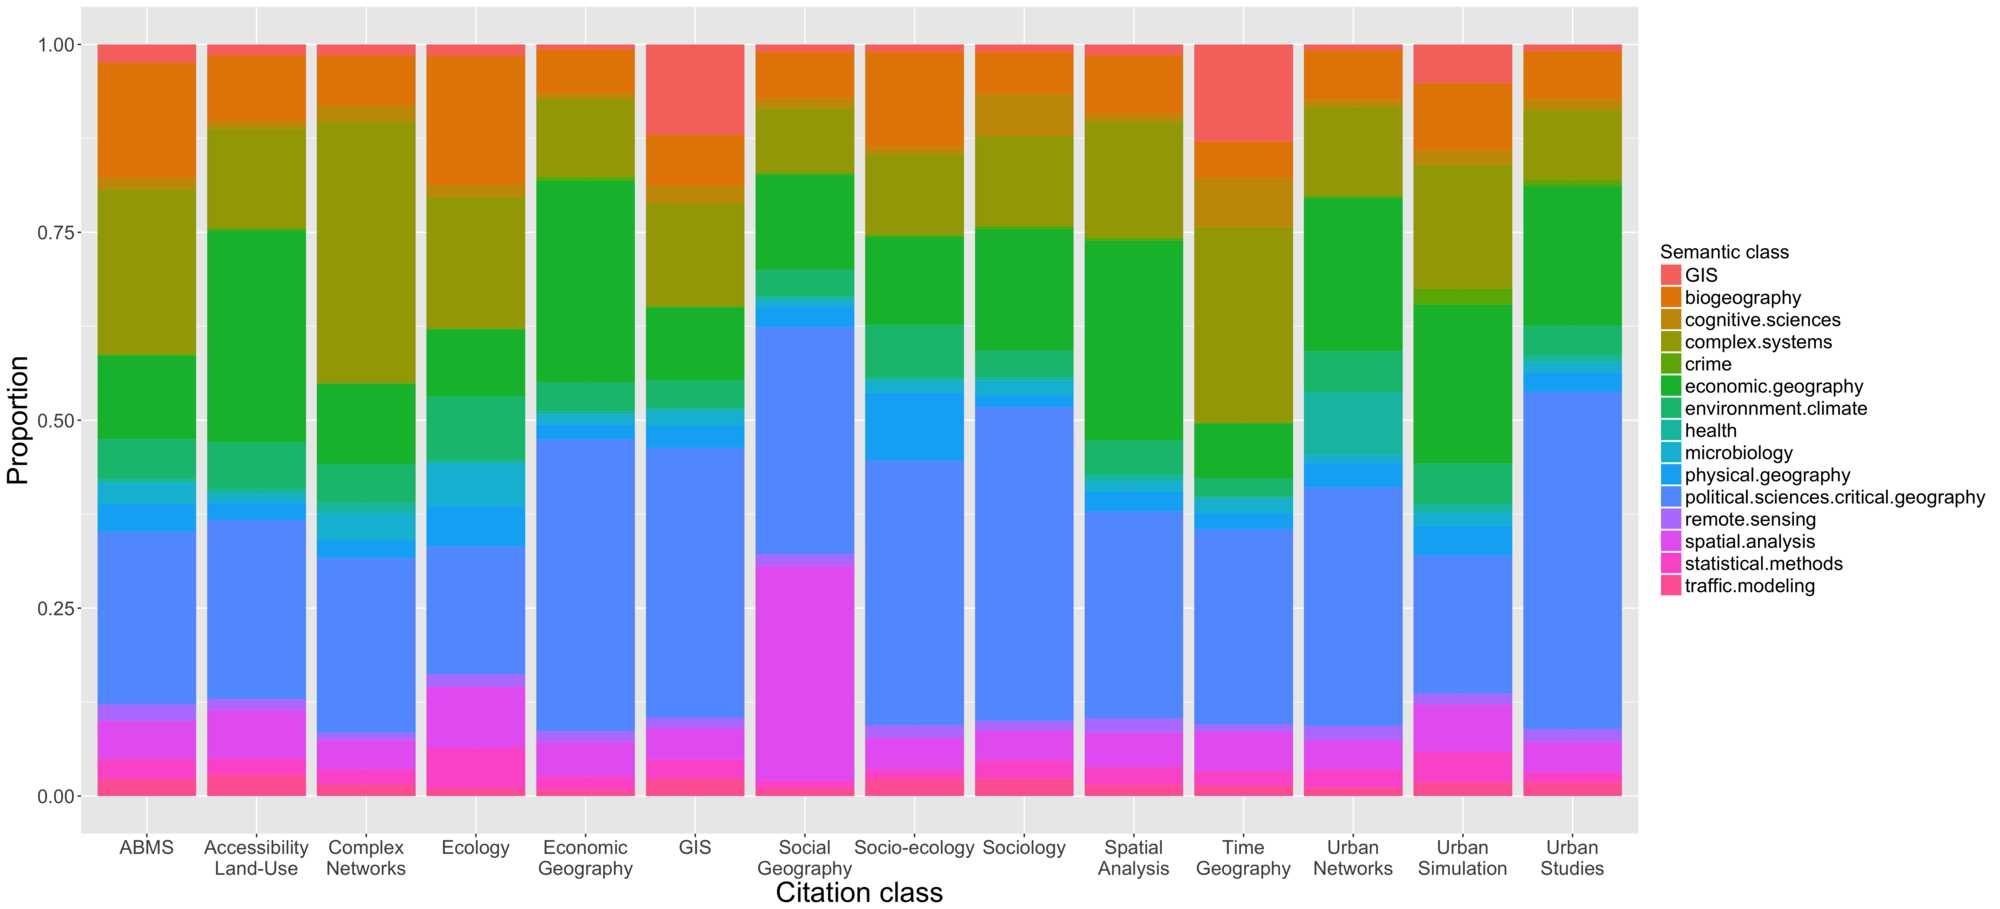
\includegraphics[width=\textwidth]{figures/scim_Fig10.jpg}


}


\sframe{Measuring interdisciplinarity}{


% We had up to now a qualitative view on interdisciplinarity patterns, by looking at the rela- tive localisation of communities within the citation and semantic classifications, and the relation between the classifications. We propose now to look at quantitative measures of interdisciplinarity, for each classification. More precisely, for a given classification C ∈ {Citation, Semantic} a reference i can be viewed as a probability vector (p(C)) on classes j that give for each class the probability to belong to it. Given this setting, we measure interdisciplinarity of one reference using Her- findhal concentration index (Porter and Rafols 2009), that can also be called an originality index. We define originality as (C) ∑ (C)2 oi =1− pij (1) j For the semantic classification, probabilities are defined as the proportion of keywords of the abstract within each semantic class. With the deterministic citation classification, each reference has only one class and the originality index is always 0. Therefore in order to be able to compare the two classification, we associate a probability to each citation class for each article as the proportion of citations received from this class. The index introduced is original, and measures interdisciplinarity as how a reference is used by different disciplines in its lifetime. Indeed, Eq. 1 yields higher values for more evenly distributed probabilities. When used with semantic probabilities, it translates the originality in terms of language used, whereas with the citation probabilities, it gives the originality in terms of domains using the reference.We show in Fig. 11 the statistical distribution for both indexes o(Semantic) and o(Citation), stratified by citation class. This allow a direct comparison between the two and also an indirect comparison by the variation of semantic distribution between citation classes. For the distribution of semantic originalities, all citation classes exhibit a similar pat- tern, that is a peak around large values and a smaller peak at zero. It means that either references are highly specialized and have keywords in one class only, or they use keywords from different classes in a quite even manner (for comparison, an abstract with half keywords in a class and half in an other gives an originality of 0.5). The most original, i.e. the most mixed, citation class, is Complex Networks, with a distribution clearly detached from others, what would confirm their use as a method with a lot of dif- ferent problems. Social Geography is from far the less original, with a large number of single class references, and an average far lower than other classes, what would mean an increased presence of compartmentalization within the associated disciplines. In terms of citation originality index, the global picture is fundamentally different, as average originality indexes are all lower than 0.4 and most of distributions show their mode in 0, meaning that most references are only cited by their own citation class. Again, Social Geography is the less original, confirming a similar behavior in terms of citation practice than in terms of research content. The most original classes in average, with a peak in large values, are Spatial Analysis and Urban Simulation: this corresponds to the fact that these class feature quite generic methods that can be applied in several fields and are cited accordingly. Complex Networks do not reach the same level, but however exhibit a peak around 0.2 and no peak in 0, together with Ecology, suggesting disciplines having still significant impact in other disciplines. To summarize, we show (1) different patterns of interdisciplinarity, depending on disciplines, in terms of scientific content (semantic) and of scientific impact (citation); and (2) a strong qualitative difference in behavior of originalities between the two clas- sifications, what suggests their complementarity.

% Correlation between classifications
%In order to strengthen the idea of a complementarity of classifications, that would each capture different dimensions of processes of knowledge production, we finally look at the correlation matrix between classifications. We use this time effective class probabil- ities for the citation classification, i.e. a vector of zeros expect with a one at the index of the class of the reference. We compute a Pearson correlation coefficient between classes k (in semantic) and k′ (in citation) as where the covariance is estimated with the unbiased estimator. The structure of the correlation matrix recalls the conclusions obtained when studyng the semantic composition of citation communities, such as GIS having a relatively high correlation with GIS (𝜌 = 0.26), or Sociology with Political Science (𝜌 = 0.16). These correlations are high regarding other values in the matrix, but remain low values in absolute. More important for our question are summary statistics of the overall matrix. It has a minimum of − 0.16 (Ecology (citation) against Political Sciences (semantic)), an aver- age of − 0.002 and a maximum of 0.33 (Social geography (citation) and Spatial Analysis (semantic)). The “high” values are highly skewed, as the first decile is at − 0.06 and the last at 0.09, what means that 80% of coefficient lie within that interval, corresponding to low correlations. In a nutshell, classifications are consistent as highest correlations are observed where one can expect them, but most of classes are uncorrelated, meaning that the classifications are quite orthogonal and therefore complementary.

\begin{center}
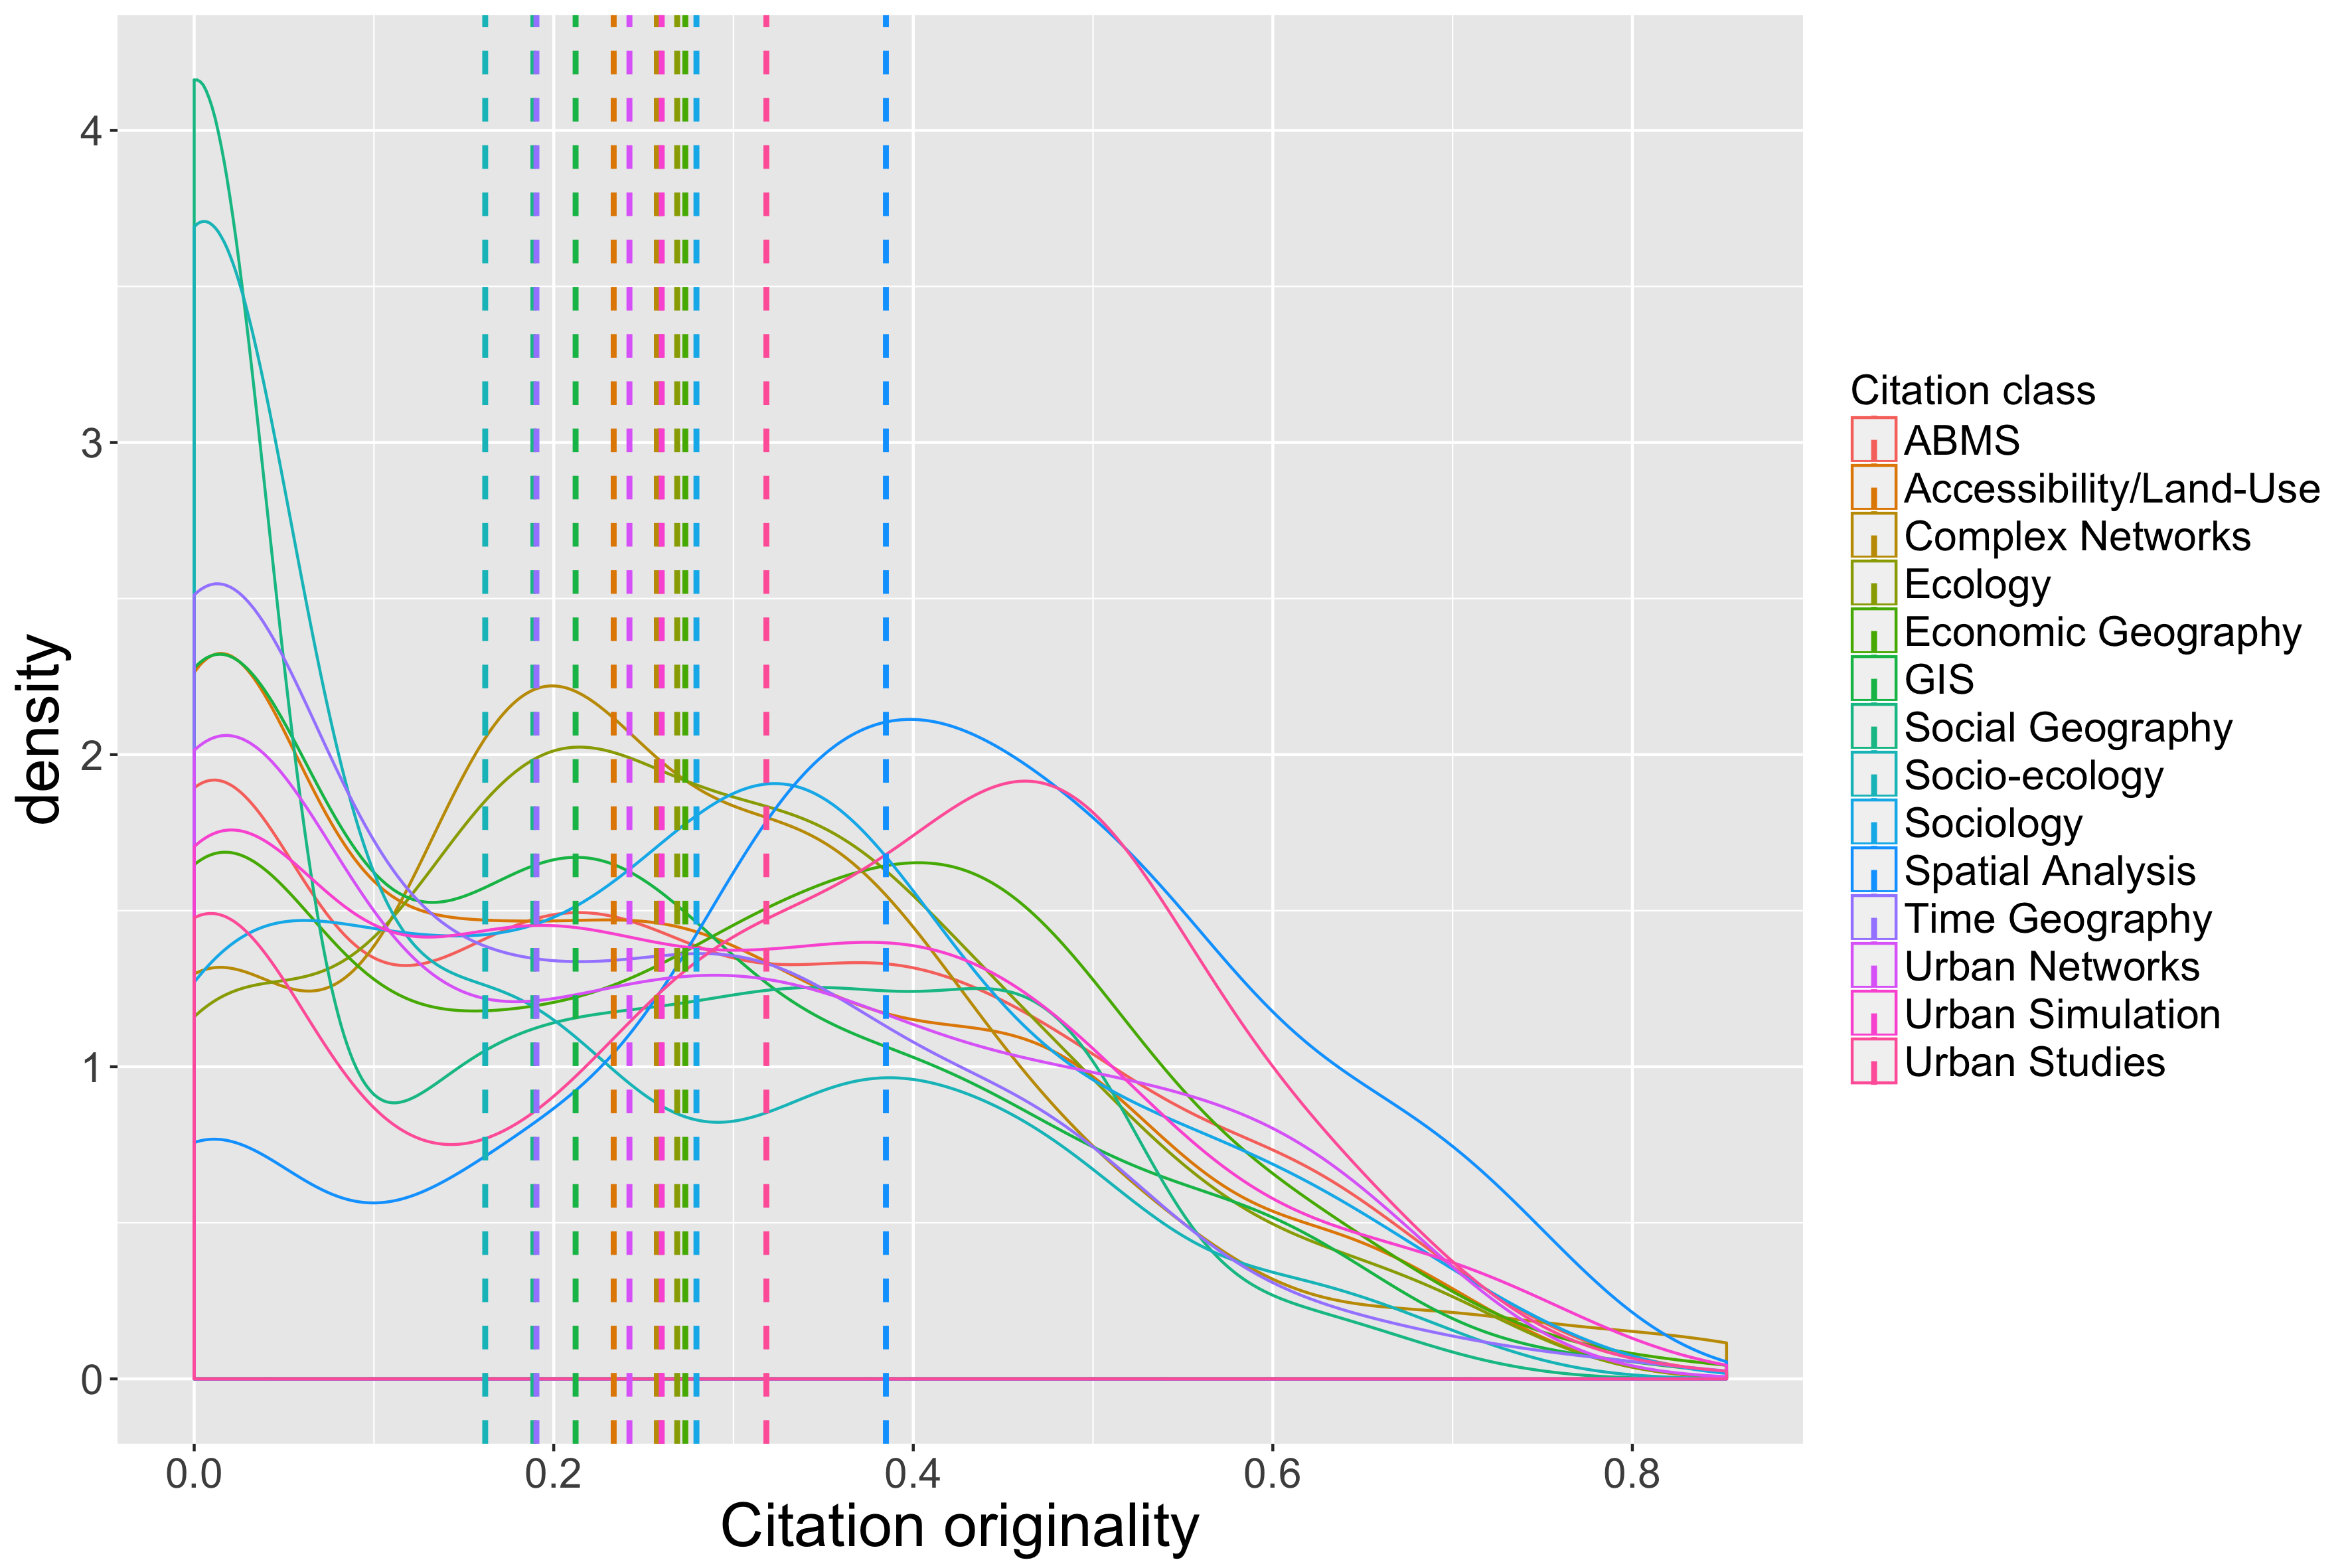
\includegraphics[width=0.8\linewidth]{figures/scim_citation_originalities_citclass.png}
\end{center}

\footnotesize
\textit{Distribution of originalities (Herfindhal index) for how references are cited by different citation classes}

}

\sframe{Measuring interdisciplinarity}{



\begin{center}
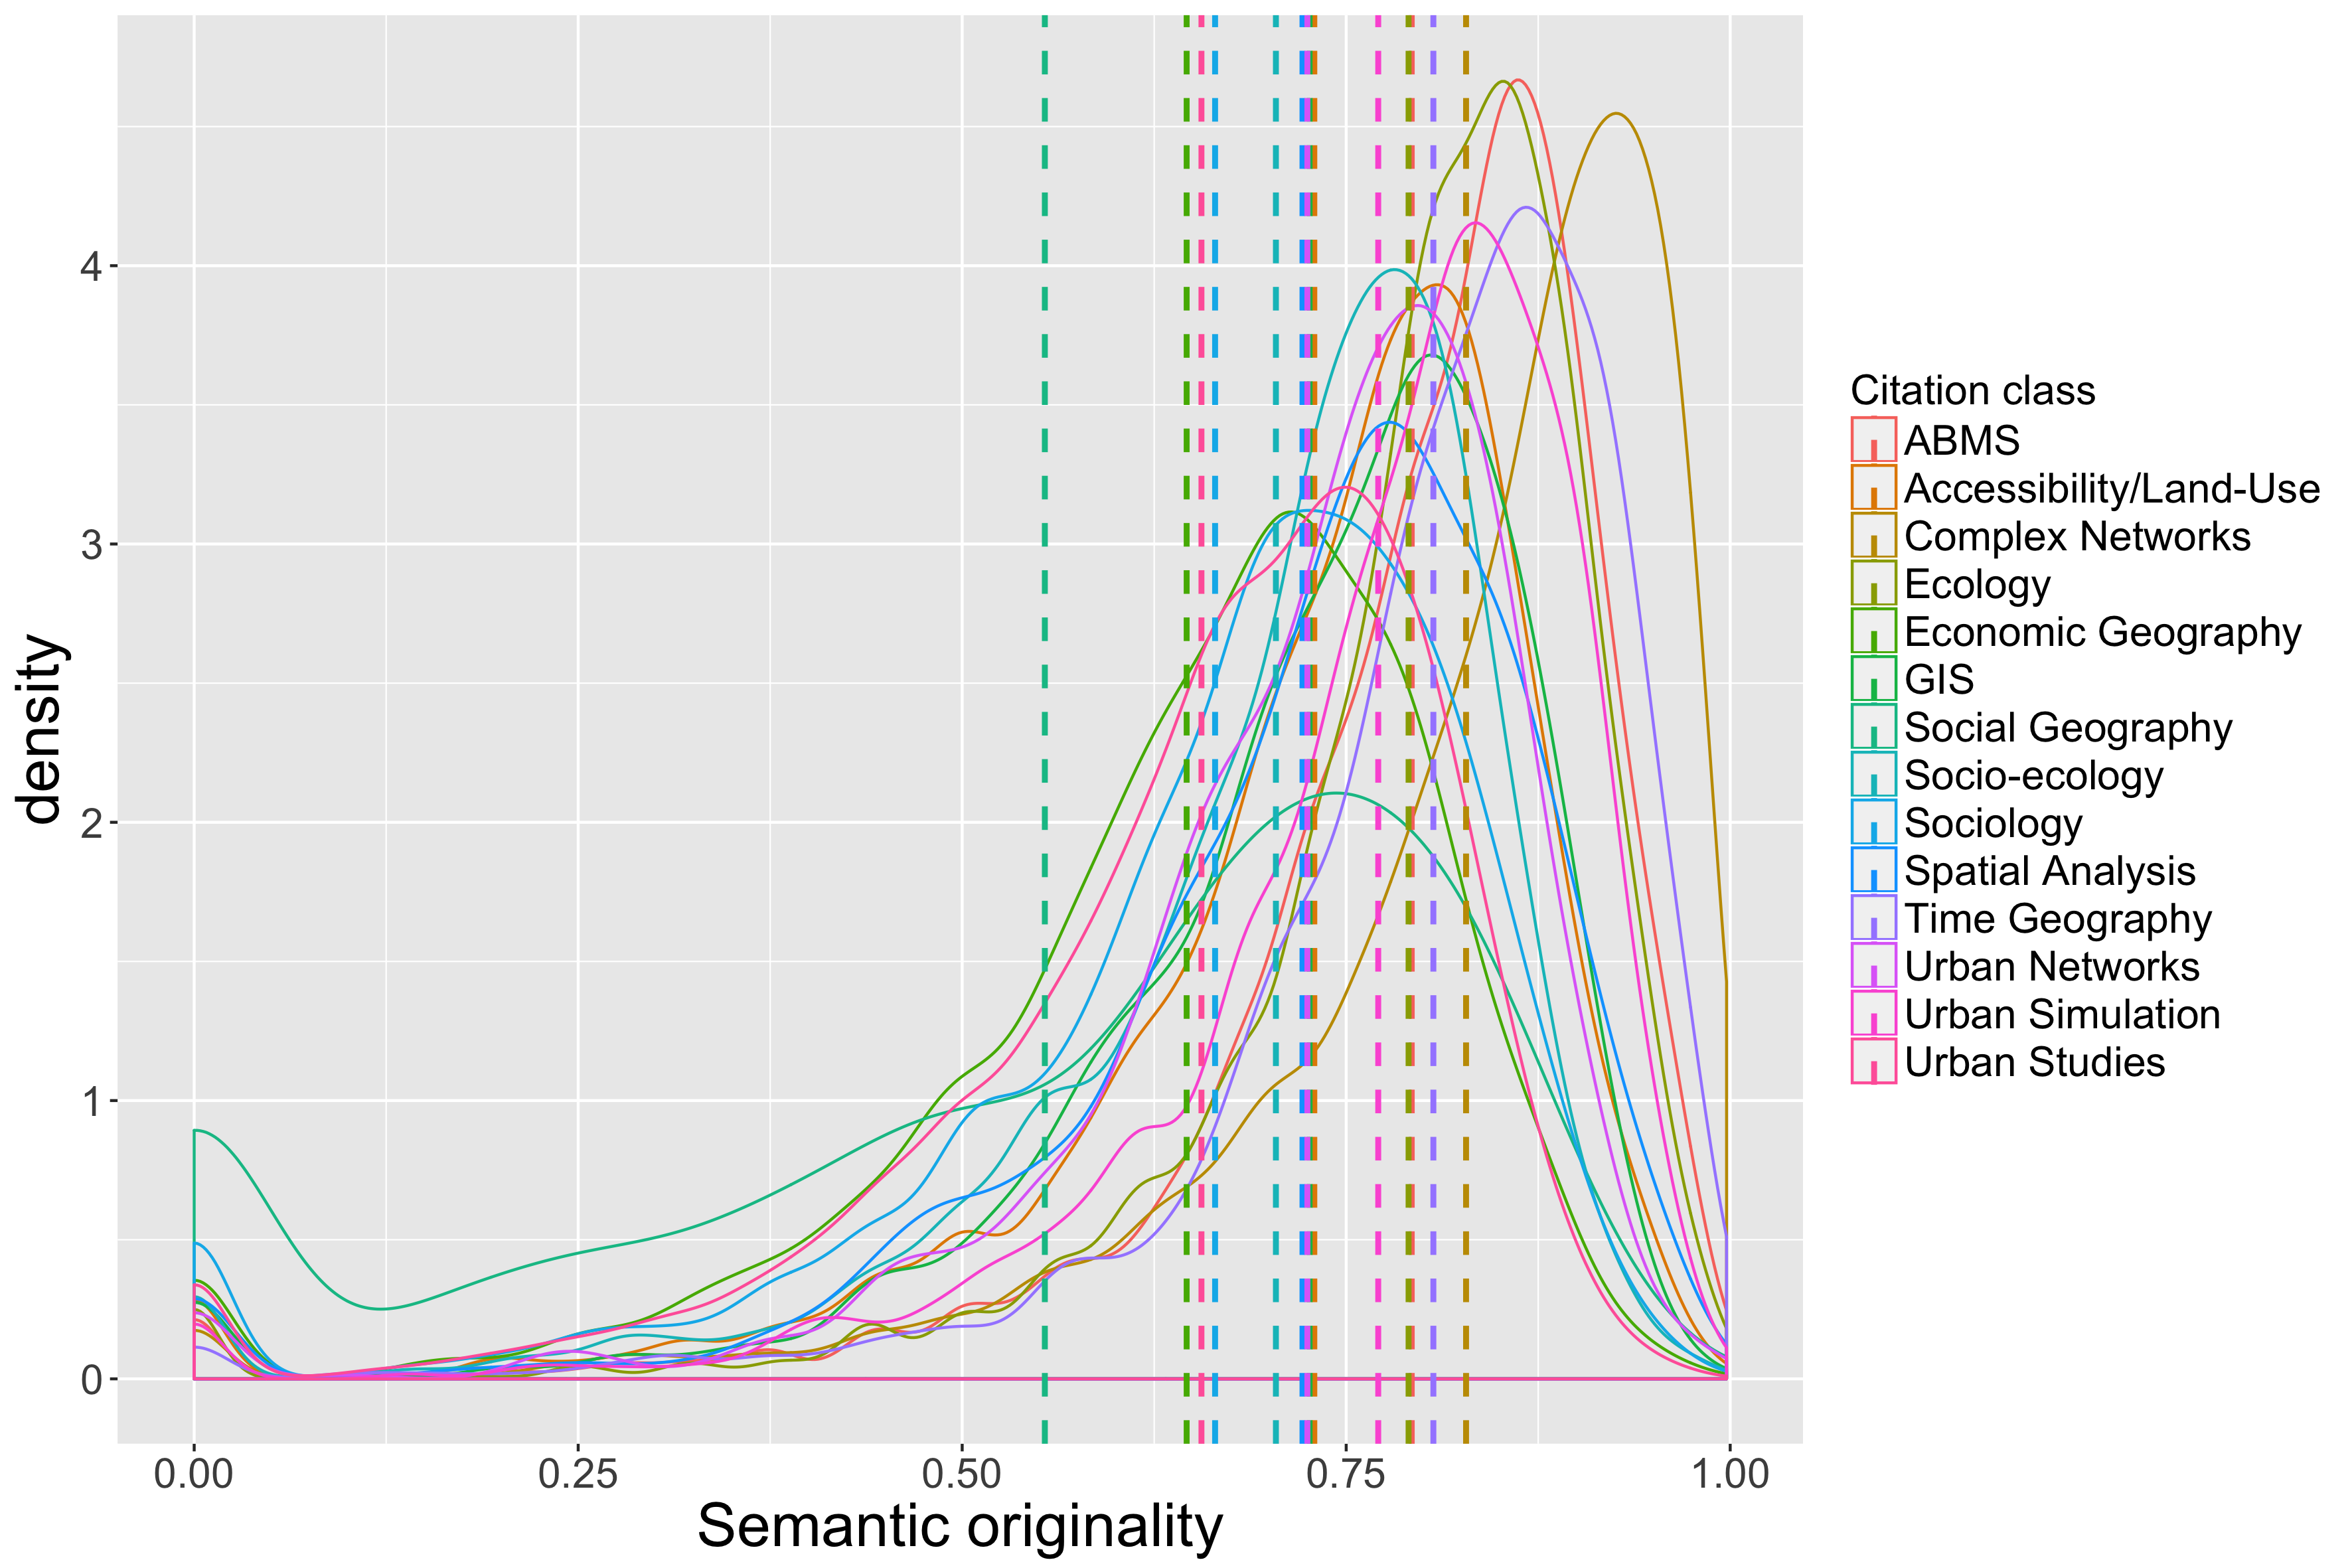
\includegraphics[width=0.8\linewidth]{figures/scim_originalities_citclass.png}
\end{center}


\footnotesize
\textit{Distribution of semantic originalities}

}


\sframe{Discussion}{

% We have this way shown the complementarity of classifications in the qualitative patterns they unveil, but also quantitatively in terms of interdisciplinarity measures and quantita- tively in terms of correlations. Our work can be extended regarding several aspects, of which we give some suggestions below.
%Developments
%A first development consists in the comparison of journals. The starting point for con- struction of the scientific environment, the journal Cybergeo, was the entry point but not the subject of our study. A development more focused on journals, trying for example to answer comparative issues, or to classify journals according to their effective level of inter- disciplinarity regarding different dimensions, would be potentially interesting. The collec- tion of precise data on the origin of references is however a first step that need to be solved first.
%The performance of the semantic classification was also not quantified here. A further validation of the relevance of using complementary information contained in both classifi- cations could be done by the analysis of modularities within the citation network, as done in Bergeaud et al. (2017). This would however require a baseline classification to compare with, which is not available in the type of data we use. Open repository such as arXiv (for physics mainly) or Repec (for Economics) provide API to access metadata including abstracts, and could be starting points for such targeted case studies.
%An other aspect on which our work could shed an interesting light is the univocity of scientific keywords between disciplines. Indeed, the same word can relate to different con- cepts in different disciplines. Co-occurrences patterns of specific words within the differ- ent citation communities should give information on the underlying concepts in each. For example, in the fields we studied, the word “model” will correspond to totally different concepts in Quantitative Geography and in Urbanism.

\justify

\textbf{Developments}

\medskip

$\rightarrow$ Journal dynamics and benchmarking, reflexivity for authors; fostering Open Science \cite{raimbault2019empowering}

\medskip

$\rightarrow$ Performance of the semantic classification for citation link prediction

\medskip

$\rightarrow$ Correspondence of terms between disciplines

\bigskip
\bigskip




% Applications
%A first potential application of our methodology relies on the facts that both classifications unveils thematic domains (objects of study), classical disciplines, methodological commu- nities. These different types of communities can indeed be understood as different Knowl- edge Domains. Raimbault (2017) postulates co-evolving Knowledge Domains in every process of scientific knowledge production, that are Theoretical, Empirical, Modeling, Methodology, Tools and Data domains. Most of them are necessary for any process, and investigations within one conditions the advances in others. A refinement of classifications, associated with supervised classification to associate knowledge domains to some com- munities (potentially using full texts to have more precise information on the proportion of each knowledge domains involved in each), would allow to quantify relations between domains. Furthermore, using temporal data with the date of publications, would yield an effective quantification of the co-evolution of domains in the sense of patterns of temporal correlations (e.g. Granger causality).
%Our work furthermore suggests that the different types of communities each unveil a different structure of science. This has implications for the construction of science maps, which refinement may go towards different maps for each dimension (which can more or less be associated to Knowledge Domains). Wen et al. (2017) have for example introduced such specific complementary maps as a new method of “bibliometric trian- gulation” in the case of water research.
%An other interesting direction is the application of our classifications to the quanti- fication of spatial diffusion of knowledge, as Maisonobe (2013) does for the diffusion of a specific question in molecular biology. It is not clear if different dimensions of knowledge diffuse the same way: for example citation practices can be correlated to social networks and thus exhibit different patterns than effective research contents. This phenomenon is suggested in terms of a co-evolution for semantics and social networks by Roth and Cointet (2010). Therefore, our work would allow to study such questions from complementary point of views.

\textbf{Applications}

\medskip

$\rightarrow$ Quantification of Domains of Knowledge \cite{raimbault2017applied}

\medskip

$\rightarrow$ Complementary dimensions in the structure of science

\medskip

$\rightarrow$ Spatial diffusion of knowledge \cite{doi:10.1162isala00283} 




}








%\sframe{Conclusion}{
%
%% We have introduced a multi-dimensional approach to the understanding of interdiscipli- narity, based on citation network and semantic network analysis. Starting from a gen- eralist journal in Geography, we construct a large corpus of the citation neighborhood, from which we extract relevant keywords to elaborate a semantic classification. We then show qualitatively and quantitatively the complementarity of classifications. The meth- odology and associated tools are open and can be reused in similar studies for which data is difficult to access or poorly referenced in classical databases.
%
%$\rightarrow$ A multi-dimensional approach to understand patterns of interdisciplinarity
%
%\bigskip
%
%$\rightarrow$ Open tools and methodology to foster Open Science
%
%
%\bigskip
%\bigskip
%
%\textbf{Paper at} \url{https://doi.org/10.1007/s11192-019-03090-3}
%
%(open version at \url{https://arxiv.org/abs/1712.00805})
%
%\bigskip
%
%\textbf{Open repositories for the paper and library}
%
%\url{https://github.com/JusteRaimbault/HyperNetwork}
%
%\url{https://github.com/JusteRaimbault/BiblioData}
%
%
%\bigskip
%
%\textbf{Data at} \texttt{http://dx.doi.org/10.7910/DVN/VU2XKT}
%
%}




\section{Cybergeo networks}


% Such a complementarity was also found by (Raimbault et al., 2021), adding further dimensions to the study of the same, such as author keywords, topics extracted using Bayesian models, or the geographical focus of papers.


\sframe{Complementarity of methods}{

\nocite{raimbault2021empowering}


\textit{Multiple methods applied to the Cybergeo corpus: keywords, LDA, citation and semantic network, geographical dimension}

\medskip

\centering

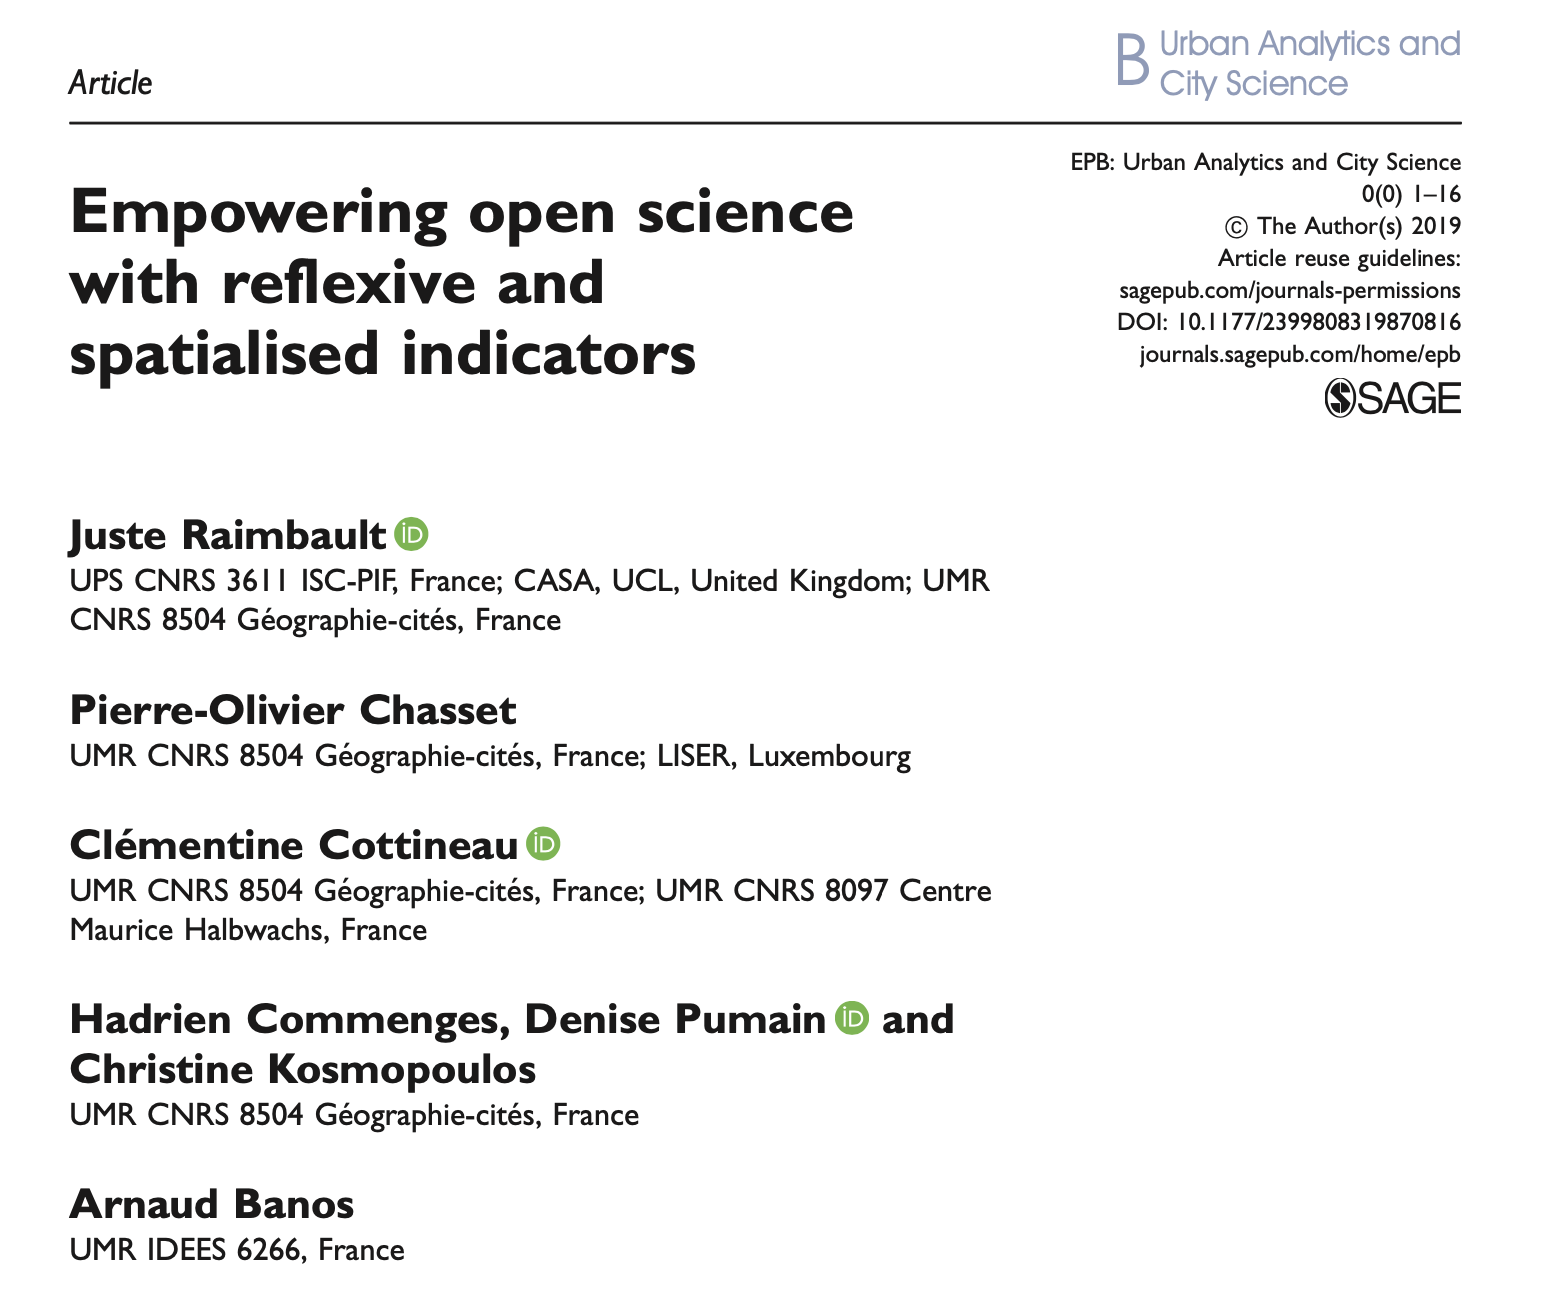
\includegraphics[width=0.6\linewidth]{figures/cyb_paper.png}

}

\sframe{Geographical content of papers}{

\centering

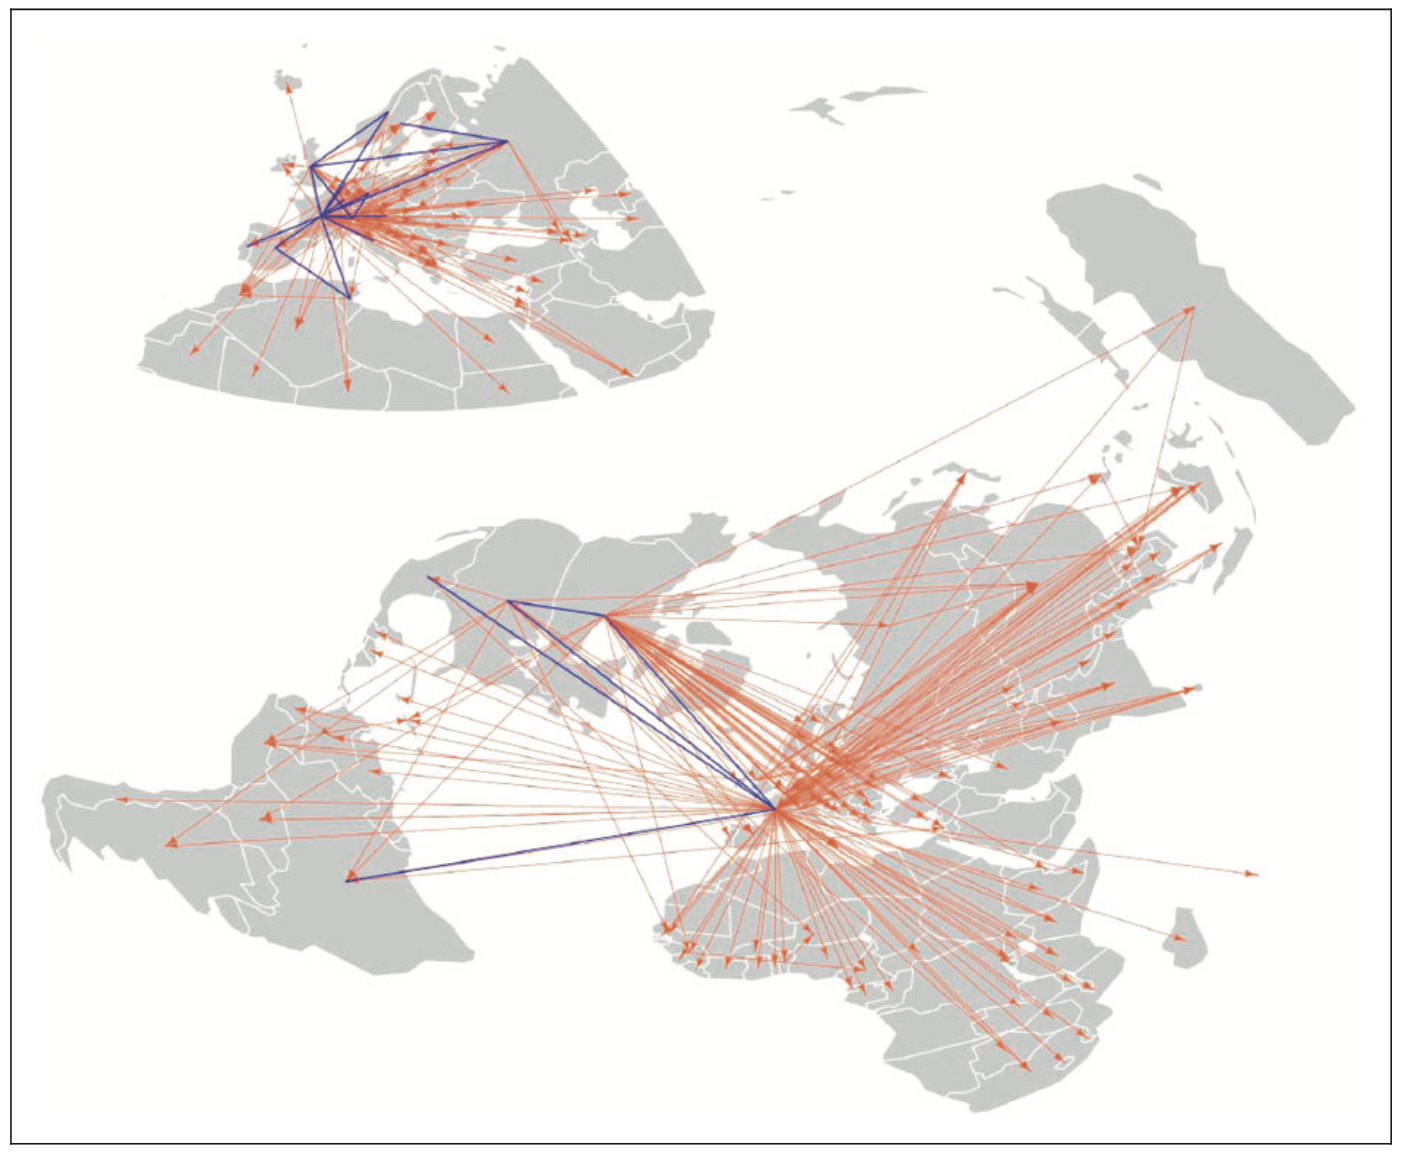
\includegraphics[width=0.8\linewidth]{figures/cyb_subject.png}

}

\sframe{Themes and their geographical distributions}{

\centering

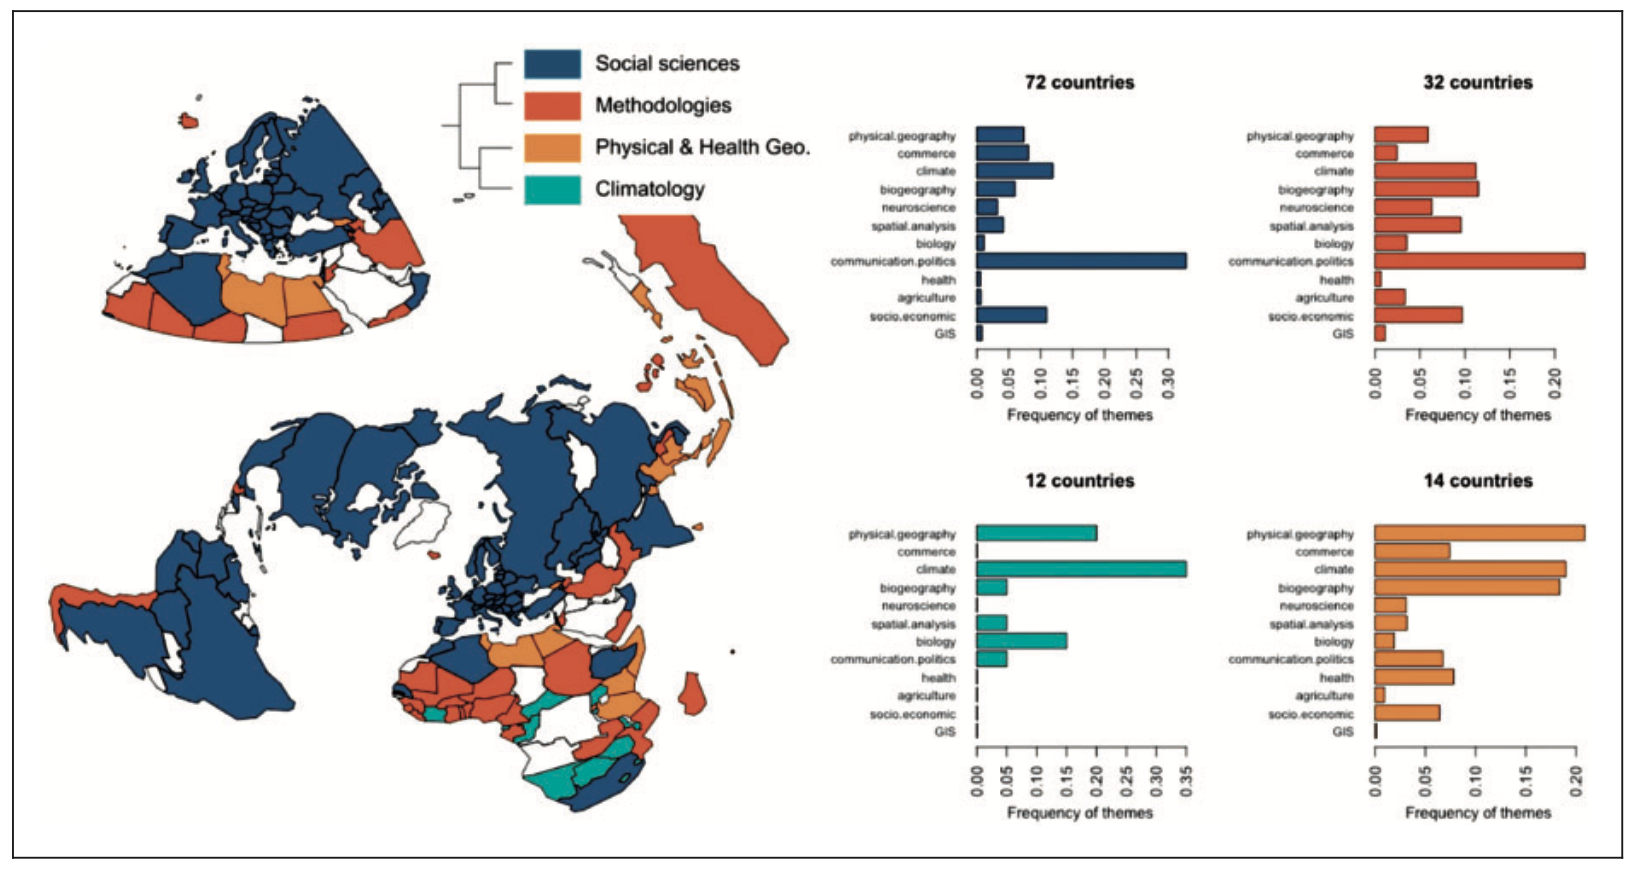
\includegraphics[width=0.62\linewidth]{figures/cyb_citation.png}\\

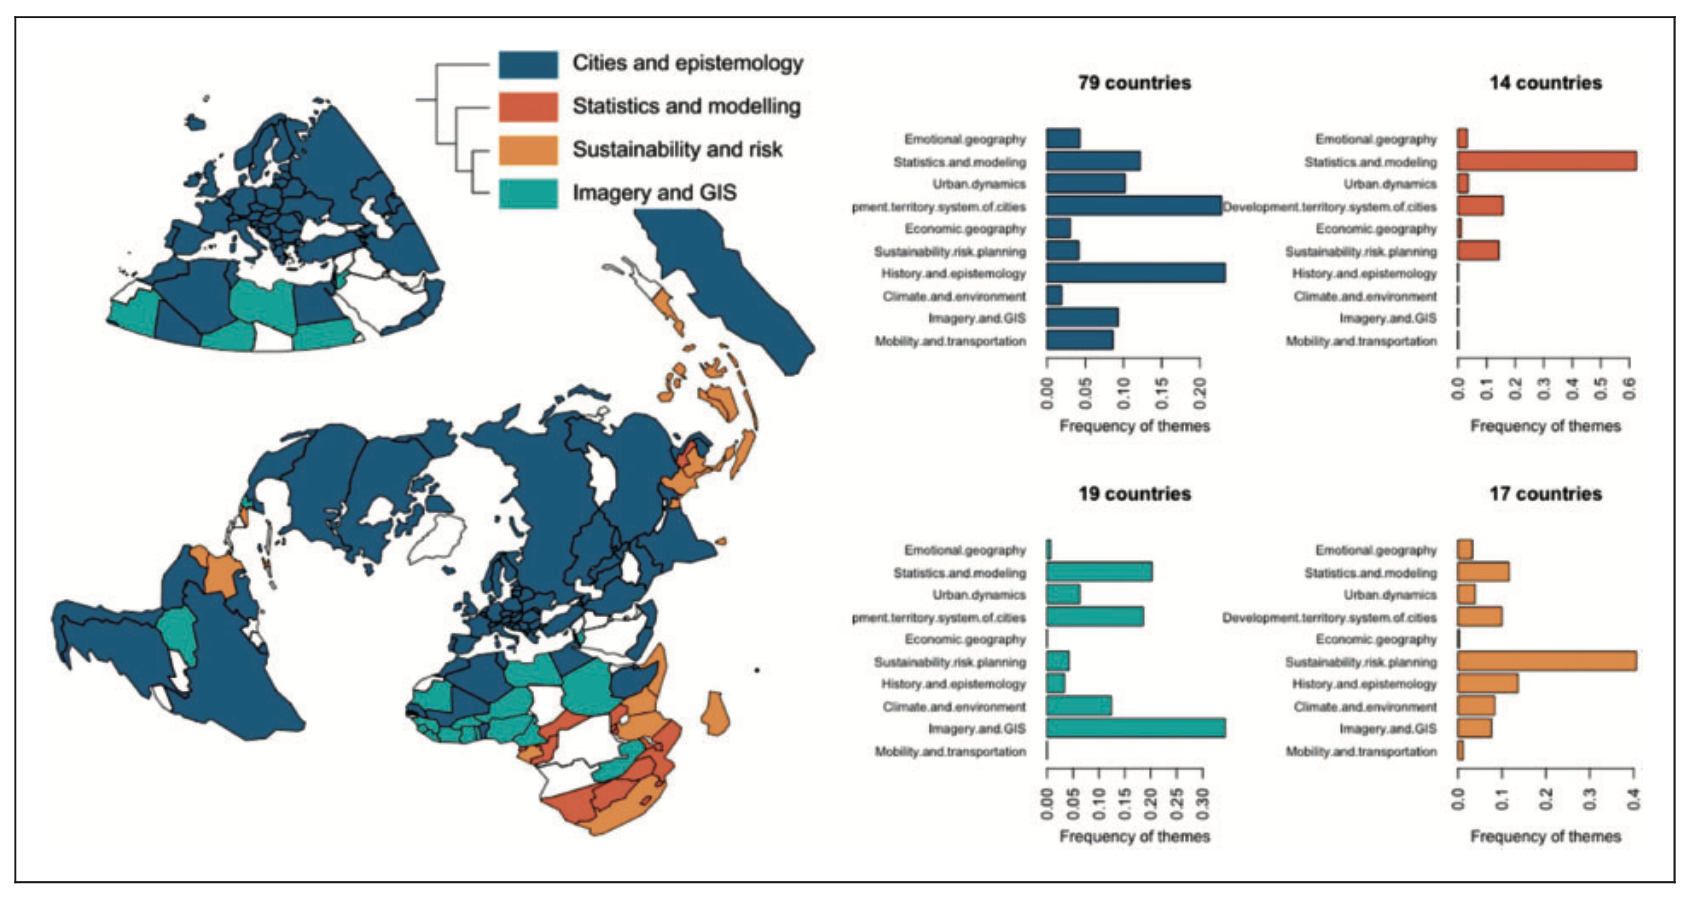
\includegraphics[width=0.62\linewidth]{figures/cyb_keywords.png}

}

\sframe{Complementarity of methods}{

\centering

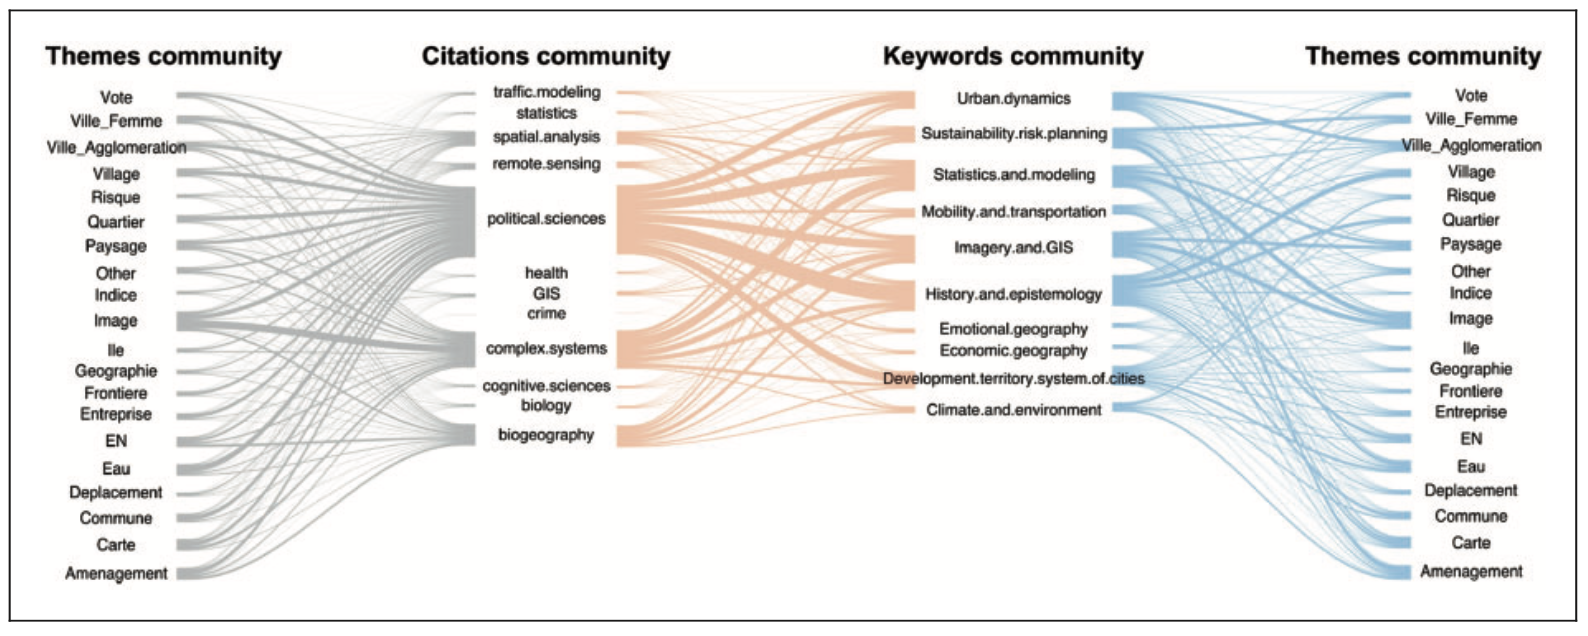
\includegraphics[width=\linewidth]{figures/cyb_flows.png}

}


\sframe{Interactive web application to foster reflexivity}{

\centering


\includegraphics[width=\linewidth]{figures/cyb_app.png}


}



\section{Geodivercity: urban perspectives}

% We then illustrate how citation network analysis can be used to obtain a reflexive view of research fields, with case studies in urban science (Raimbault and Pumain, 2020) 



\sframe{Multiple urban perspectives}{

\textit{Citation network analysis of the scientific neighborhood of perspectives developed in the Geodivercity ERC book}


\medskip

\centering

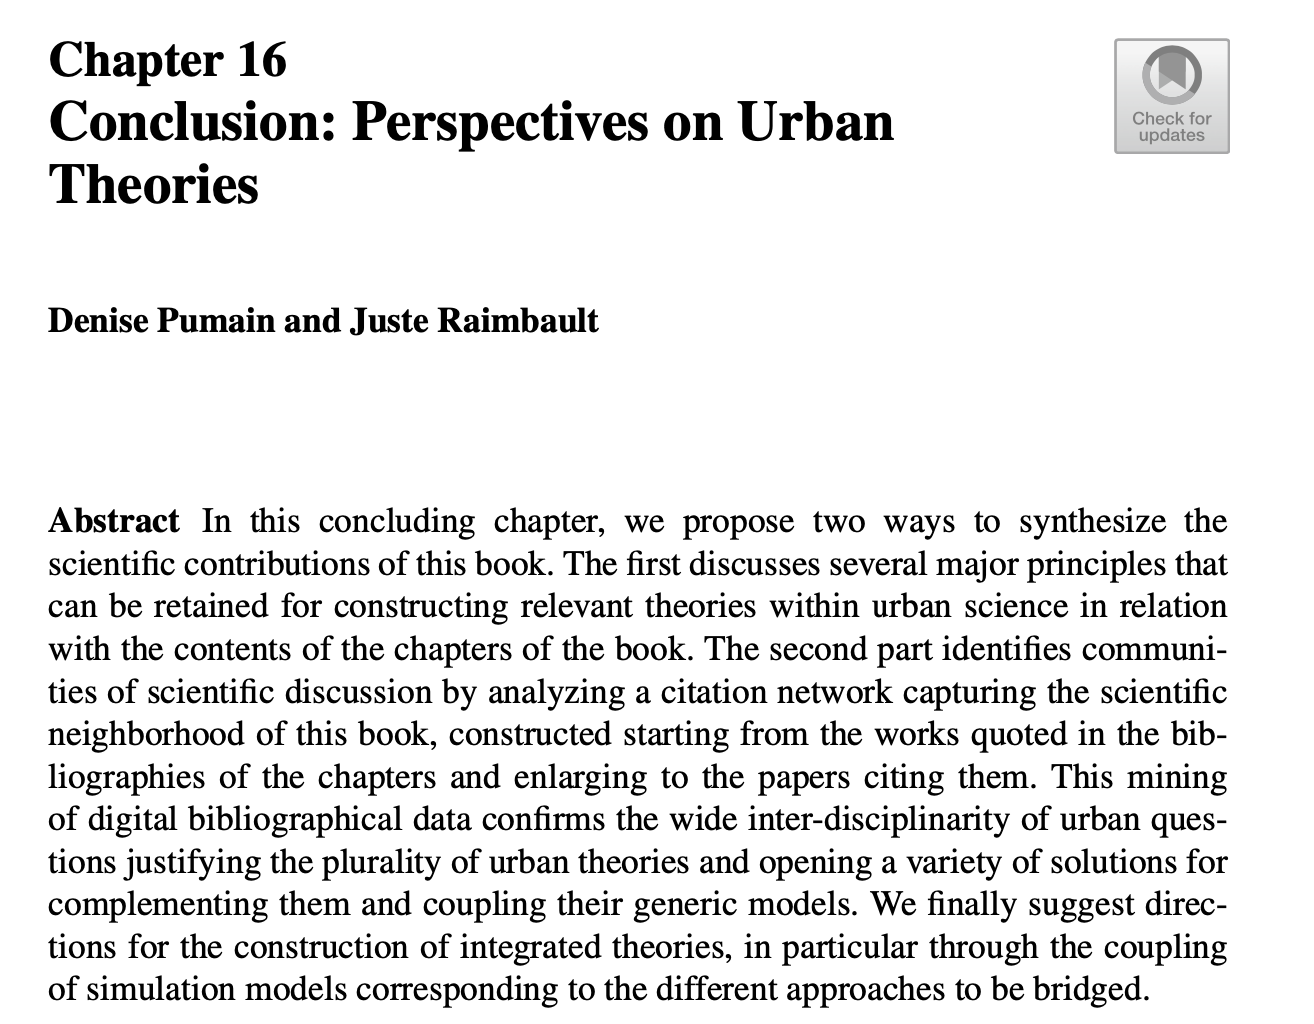
\includegraphics[width=0.7\linewidth]{figures/urbpersp_paper.png}

}

\sframe{Citation network}{

\centering

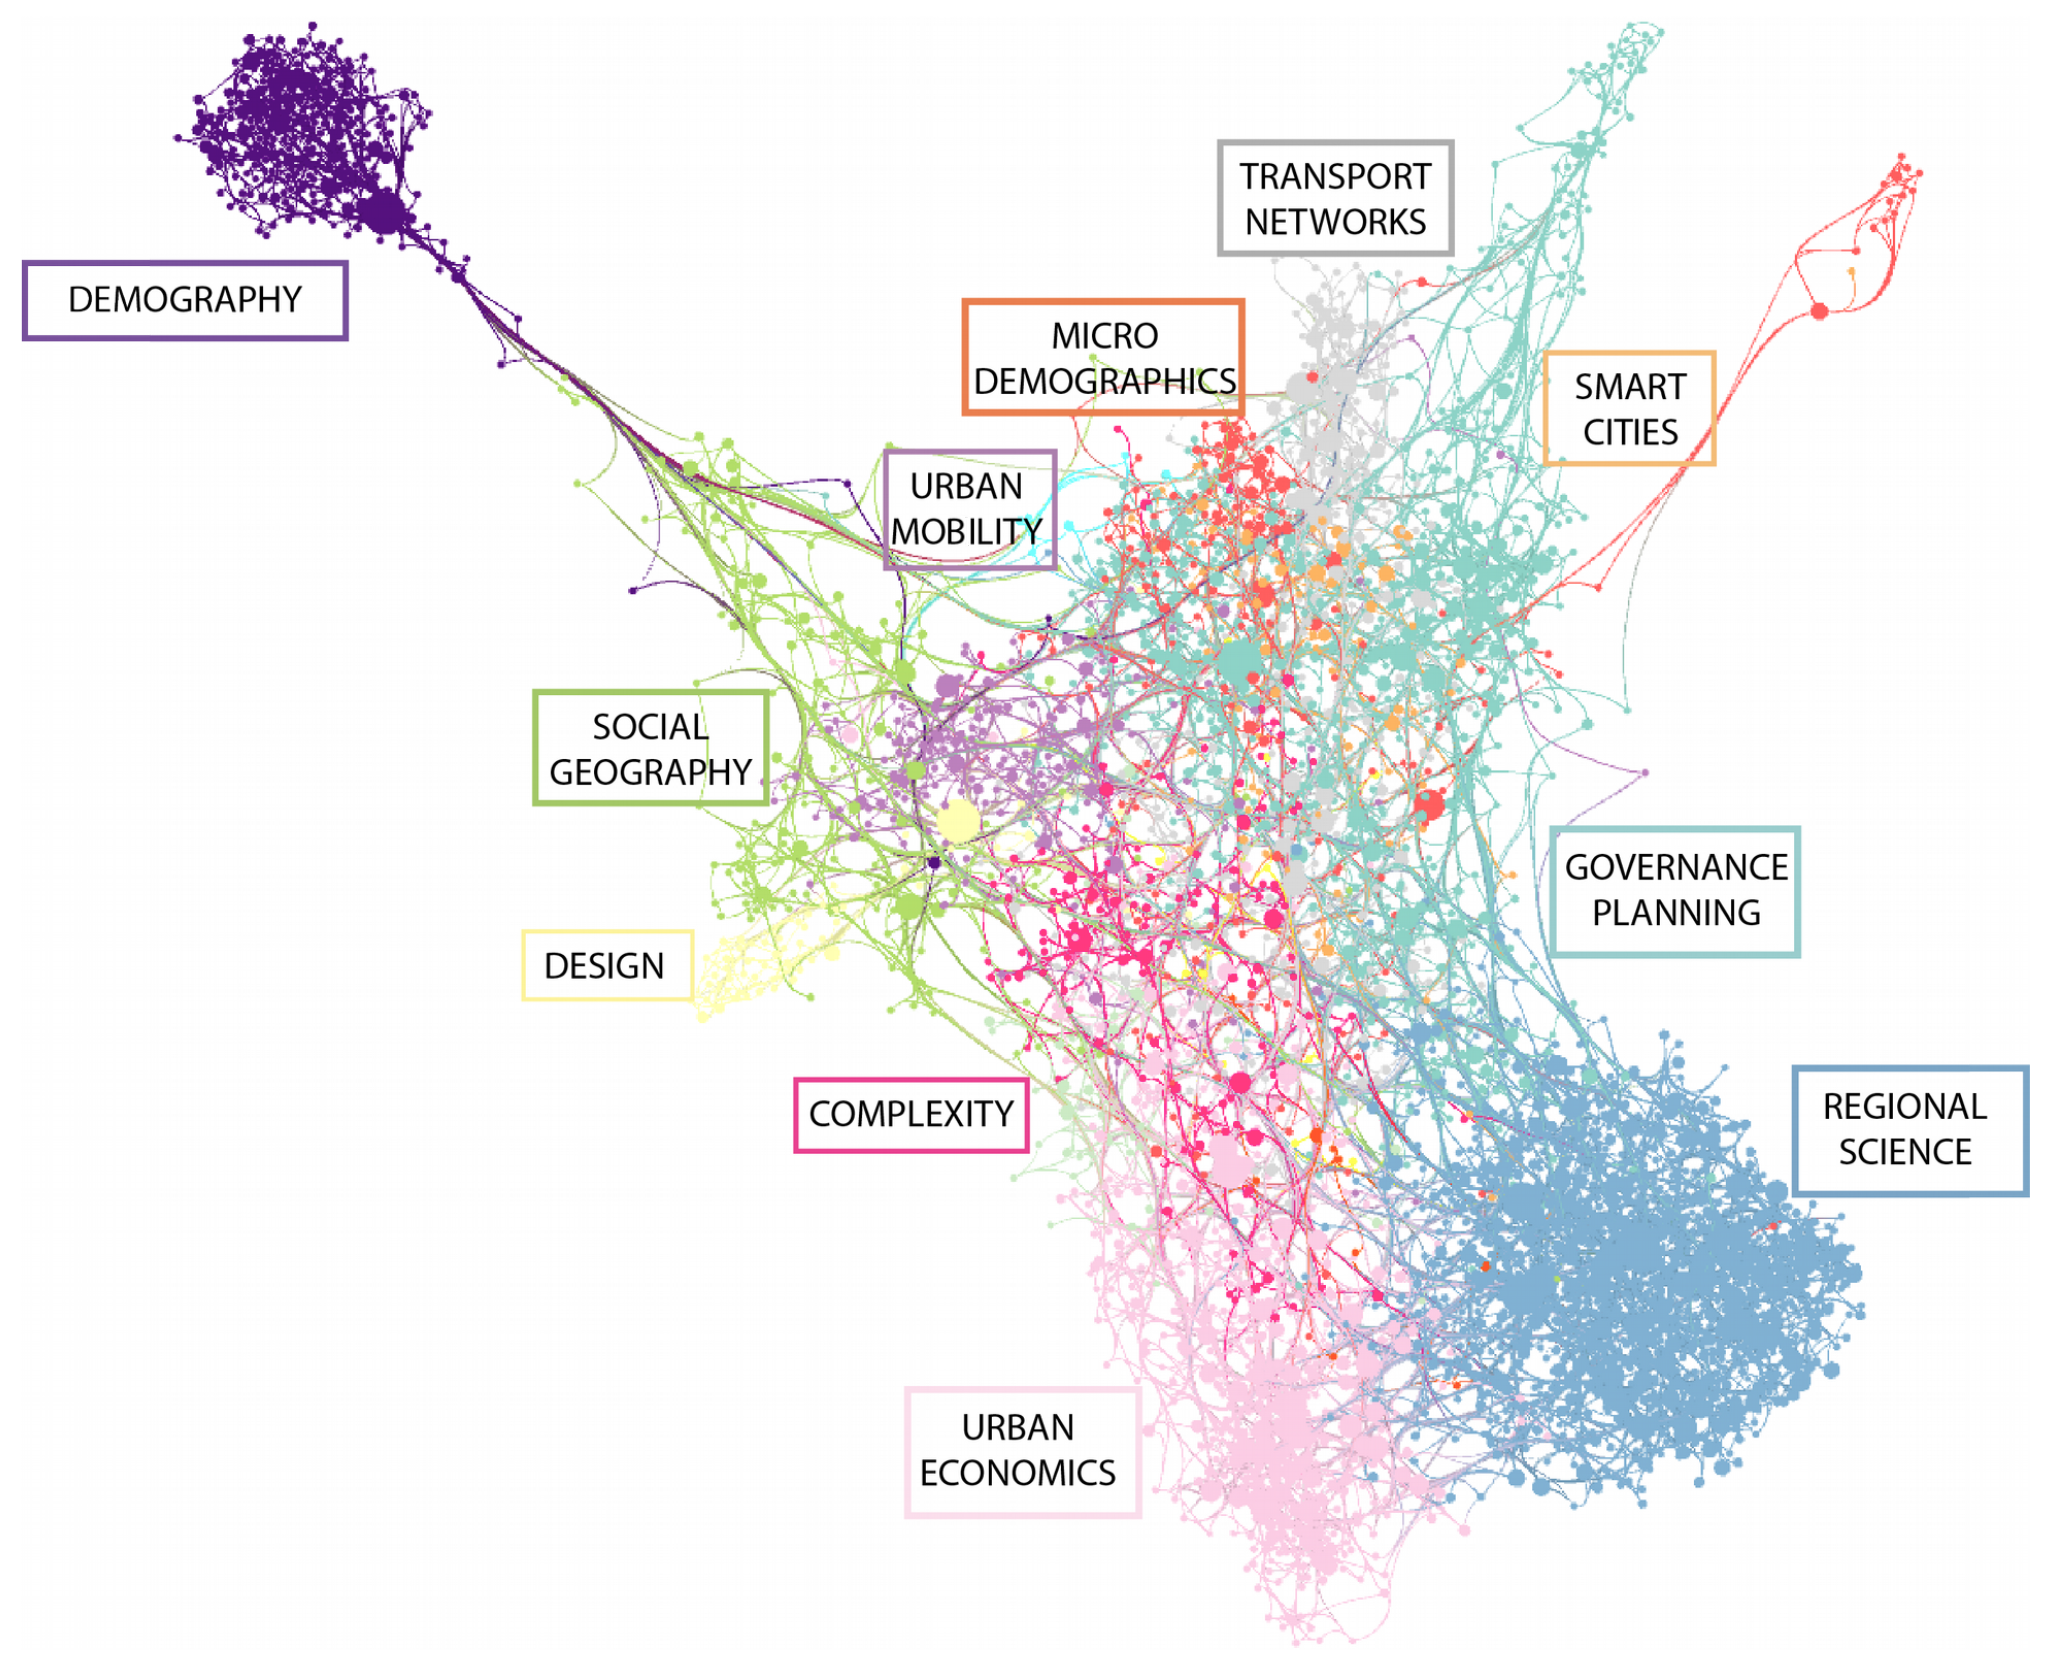
\includegraphics[width=0.9\linewidth]{figures/urbpersp_urban-perspectives.png}


}




\section{ALife and urban systems}

%and artificial life studies of urban systems (Raimbault, 2020). 



\sframe{Artificial life and urban systems}{

\begin{center}
	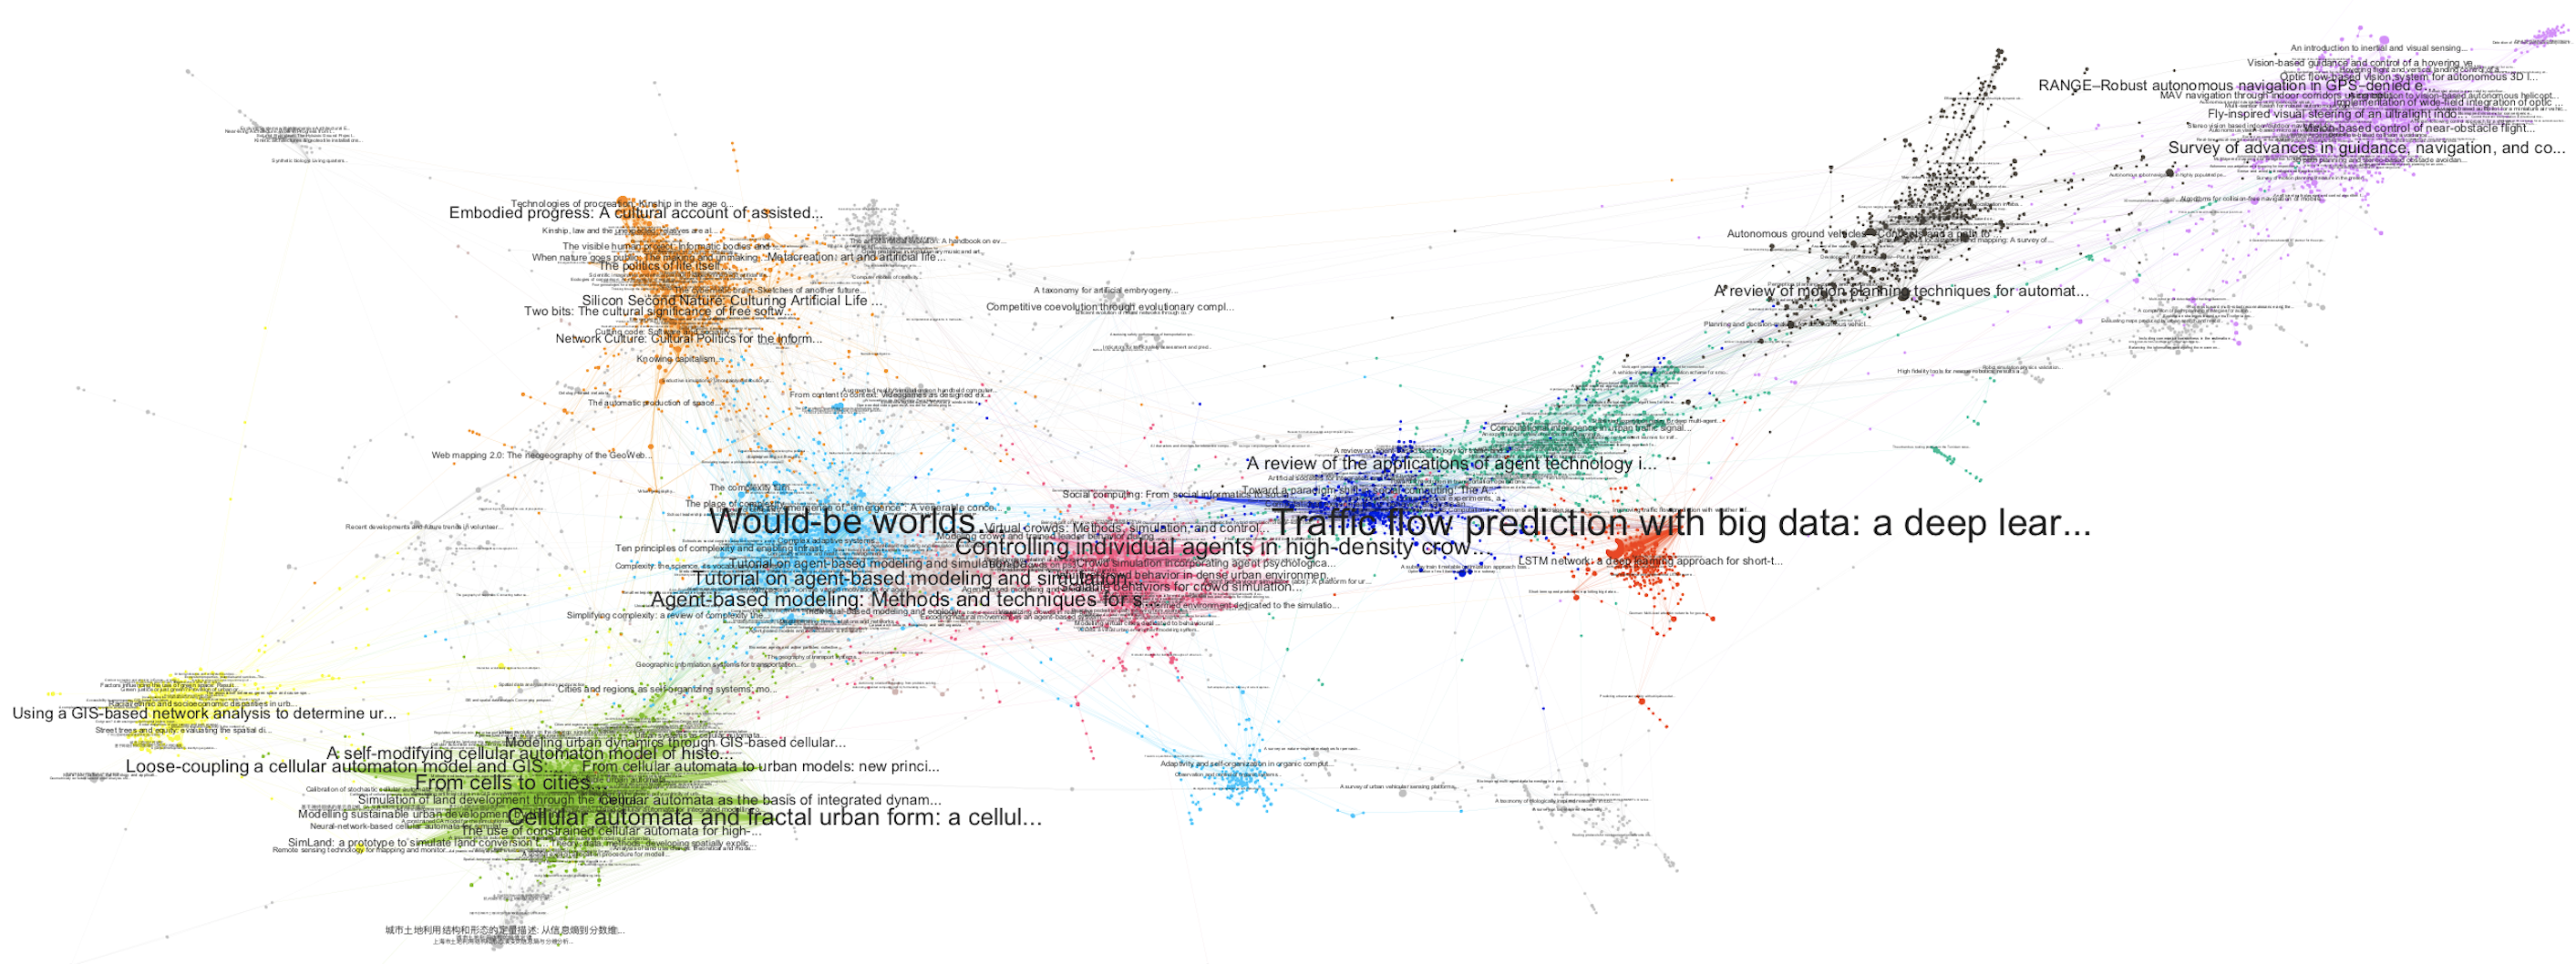
\includegraphics[width=\linewidth]{figures/alife_corealife_zoom.png}
\end{center}

\medskip

{\footnotesize \textit{Citation network of ALife studies of urban systems} \nocite{raimbault2020cities}}

\bigskip

\textbf{Transfer of concepts: } Urban morphogenesis, bio-inspired design, urban ecology, autopoiesis \cite{batty2009evolution}


%\textbf{Generative social science: } generating an emerging phenomenon from the bottom-up provides explanations \cite{epstein2006generative}

\medskip

\footnotesize

Raimbault, J. (2020). Cities as they could be: Artificial life and urban systems. arXiv preprint arXiv:2002.12926.

}



\section{Towards a quantification of a knowledge framework}

% We conclude by recalling the knowledge framework introduced by (Raimbault, 2017) for the study of complex systems, and propose a research project towards its quantification using network science, with the potential to further enhance open science and reflexivity.



\sframe{Knowledge Frameworks}{


\justify

\vspace{-0.5cm}

\textbf{Knowledge Framework : } \textit{A systemic framework containing an epistemological component dealing with the nature of knowledge or knowledge production.}

\bigskip

$\rightarrow$ Knowledge management: \cite{durantin2016disruptive} coupling engineering with design paradigms; \cite{carlile2004transferring} knowledge at the boundaries of disciplines.

\medskip

$\rightarrow$ Meta-modeling frameworks: \cite{cottineau2015modular} multi-modeling; \cite{golden2012modeling} unified formal description of Complex Systems.

\medskip

$\rightarrow$ Applied frameworks: \cite{2017arXiv170401407M} typology of approaches in Artificial Intelligence.

}


\sframe{Iterative Construction of Knowledge across Domains}{

\centering

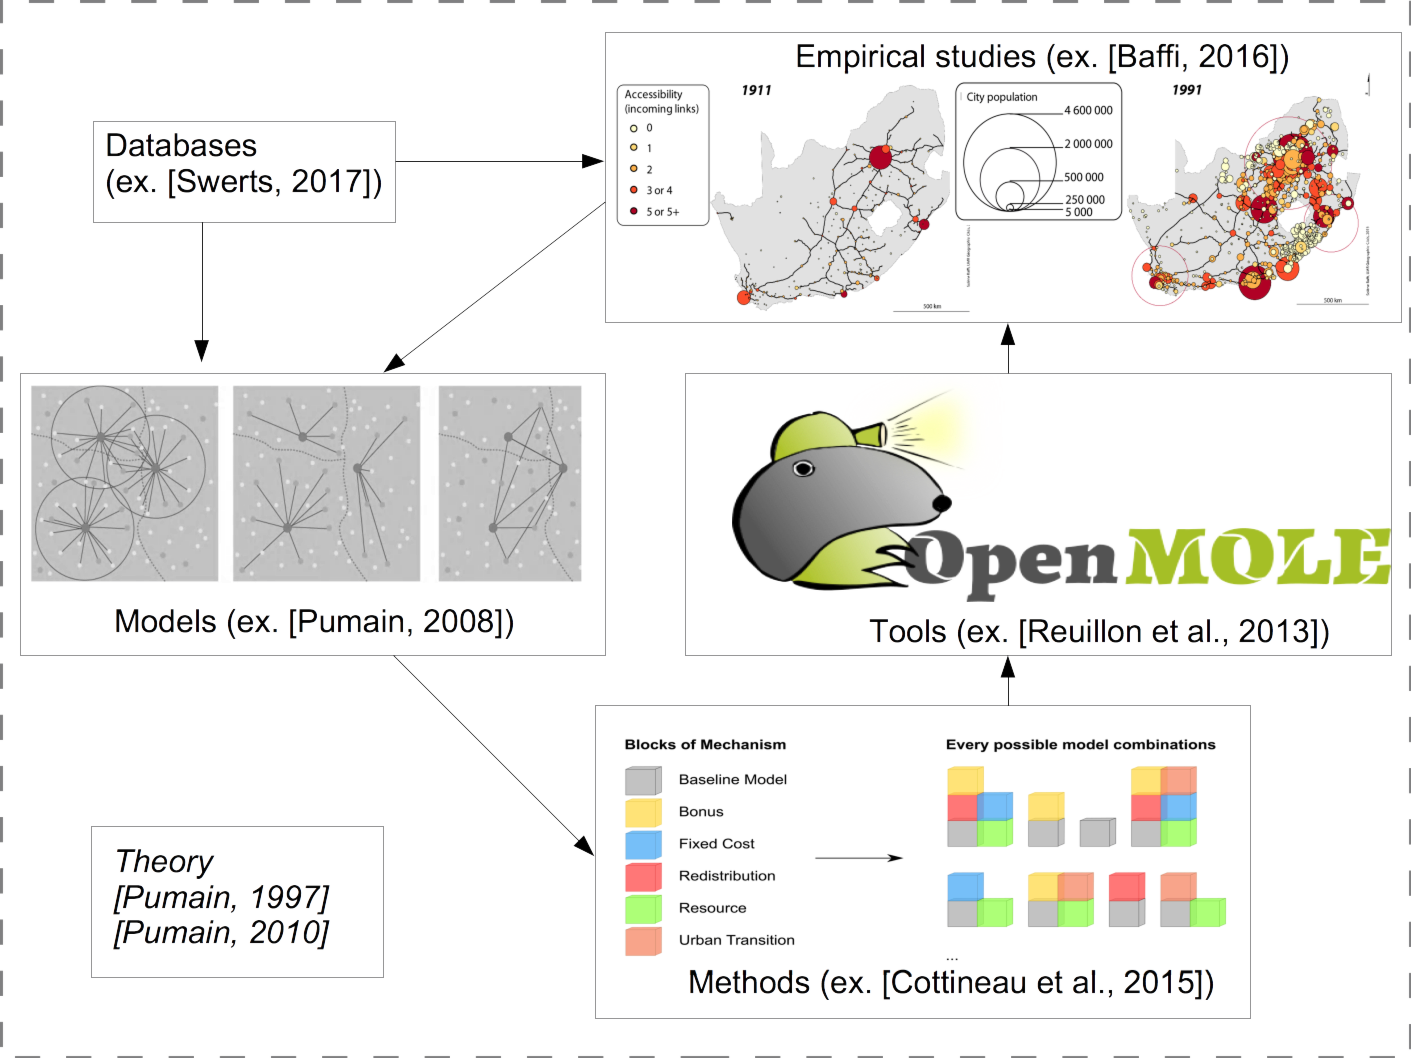
\includegraphics[height=0.9\textheight]{figures/kf_openmoleslide}


\nocite{baffi:tel-01389347}
\nocite{pumain2008socio}
\nocite{reuillon2013openmole}
\nocite{cottineau2015modular}
\nocite{swerts2017database}
\nocite{pumain1997pour}
\nocite{pumain2010theorie}

}



\sframe{Citation Network Analysis}{

\begin{columns}

\column{0.8\textwidth}
\centering
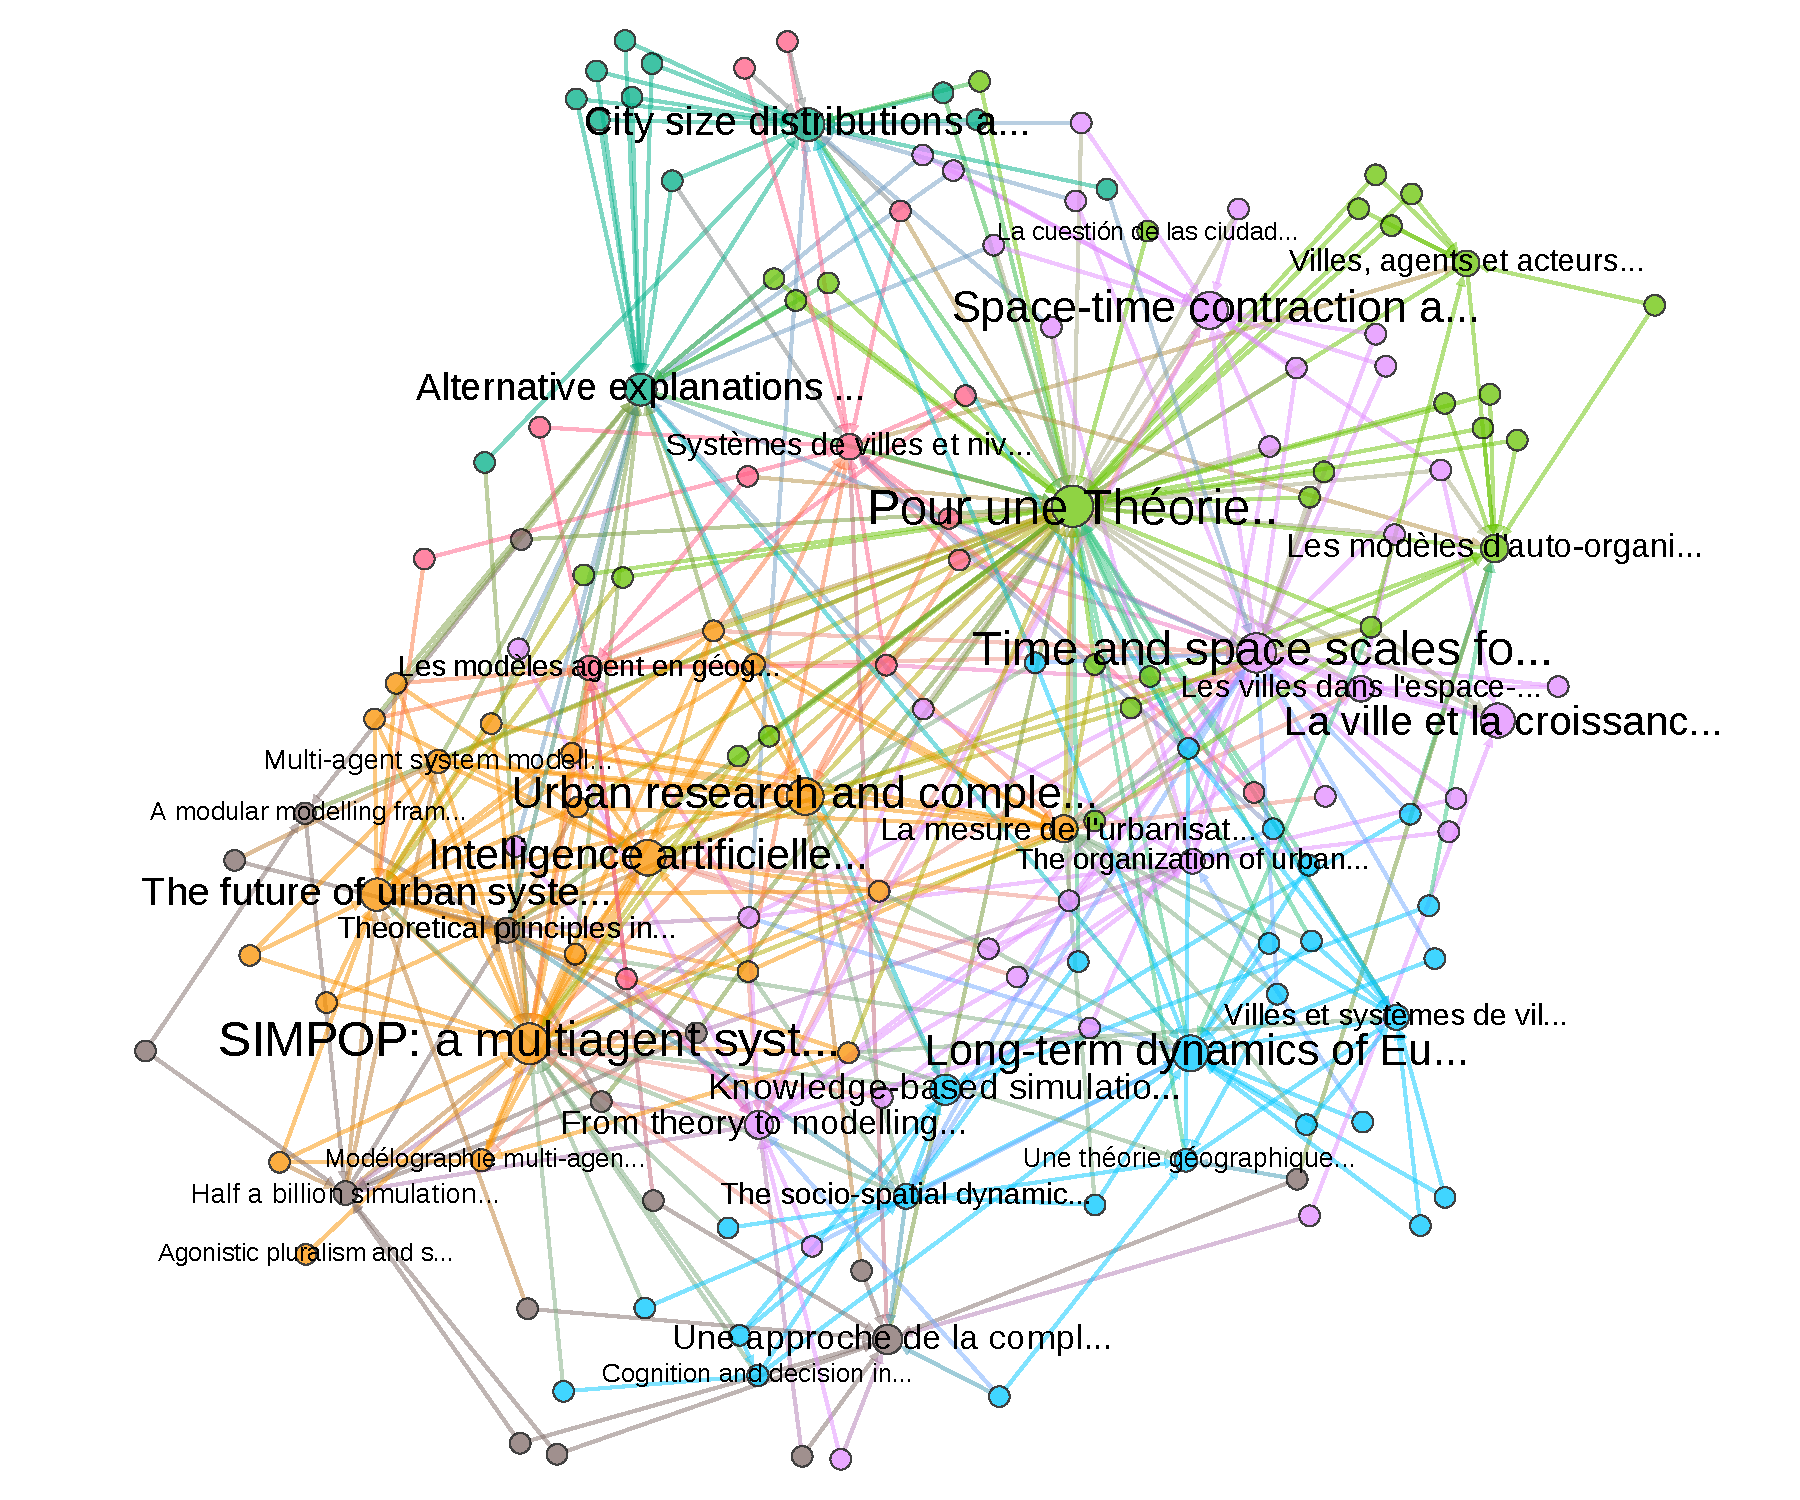
\includegraphics[width=\textwidth]{figures/kf_core}

\column{0.25\textwidth}
\justify
\textit{Core citation network of Evolutive Urban Theory}

\smallskip

$\left|V\right| \textrm{=} 155$

$\left|E\right| \textrm{=} 449$

\smallskip

7 communities, modularity 0.39

\end{columns}

}


\sframe{Knowledge Domains}{

% We postulate the following knowledge domains, with their definitions:

\textit{Definition of Knowledge Domains, extending \cite{livet2010ontology}}

\begin{itemize}
\item \textbf{Empirical.} Empirical knowledge of real world objects
\item \textbf{Theoretical.} Conceptual knowledge, implying cognitive constructions
\item \textbf{Modeling.} The model as the formalized \emph{medium} of the perspective \cite{giere2010scientific}
\item \textbf{Data.} Raw information that has been collected
\item \textbf{Methods.} Generic structures of knowledge production
\item \textbf{Tools.} Implementation of methods and supports of others domains % Proto-methods
\end{itemize}

%We choose to keep separate Methods and Tools, to insist on the support role of tools, and because development of both are related but not identical. The same way, Data domain and Empirical Domain are distinct, as new datasets do not systematically imply new knowledge of empirical facts, although constructing the data captation tool implies sometimes empirical knowledge. The Modeling Domain has a central role as we postulate that, following~\cite{giere2010agent}, \emph{any knowledge on a complex system requires a model}. 


}


\sframe{Knowledge framework}{

% note: shouldnt be only pairwise interactions!

\centering

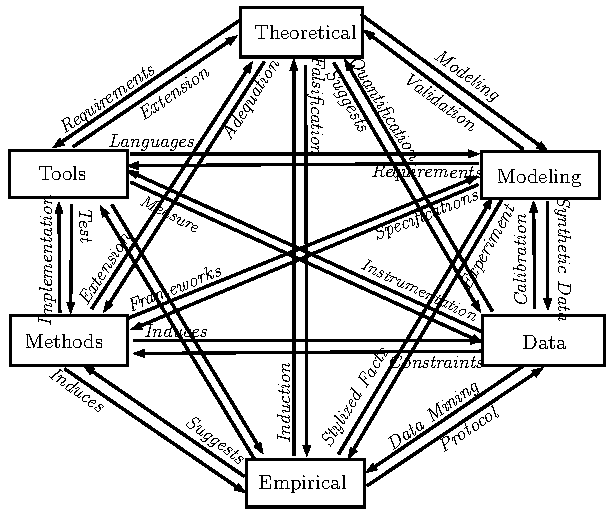
\includegraphics[height=0.9\textheight]{figures/kf_framework}


}


\sframe{Towards a quantification}{


$\rightarrow$ Citation and semantic network analysis can \textit{in some cases} provide insights into types of papers (data, methodological, case study, model)

\medskip

$\rightarrow$ Semi-supervised approach with full-texts to quantify knowledge domains \textit{within} papers

\medskip

$\rightarrow$ Dynamics of knowledge domains (see e.g. reflexive analysis in \cite{raimbault2018caracterisation}

\bigskip

\textbf{Issues:}

\begin{itemize}
	\item Practices (and domains) specific to disciplines - transferability and comparability?
	\item Limitations of machine learning regarding interpretations
	\item Data: open access papers, sci-hub?
\end{itemize}




}







\section{Conclusion}


% \url{https://github.com/JusteRaimbault/HyperNetwork}

%\url{https://github.com/JusteRaimbault/BiblioData}


\sframe{Conclusion}{


$\rightarrow$ Network analysis provides useful theoretical (knowledge production) and practical (literature mapping) insights

\bigskip

$\rightarrow$ Complementarity of methods

\bigskip

$\rightarrow$ Open tools and methodologies to foster Open Science and reflexivity


\bigskip
\bigskip


\textbf{Some open repositories}

\medskip

Patents: \url{https://github.com/JusteRaimbault/PatentsMining}

\medskip

Data collection: \url{https://github.com/JusteRaimbault/BiblioData}

\medskip

Interdisc.: \url{https://github.com/JusteRaimbault/HyperNetwork}

\medskip

Cybergeo: \url{https://github.com/Geographie-cites/cybergeo20}



}




%%%%%%%%%%%%%%%%%%%%%
\begin{frame}[allowframebreaks]
\frametitle{References}
\bibliographystyle{apalike}
\bibliography{biblio}
\end{frame}
%%%%%%%%%%%%%%%%%%%%%%%%%%%%



%\sframe{Reserve slides}{
%
%\Huge
%
%\centering
%
%Reserve slides
%
%}



\end{document}

